%%%%%%%%%%%%%%%%%%%%%%%%%%%%%%%%%%%%%%%%%%%%%%%%%%%%%%%%%%%%%%%%%%%%%%%%%%%%%%%%%%%%%%%%%%%
%%
%% The updated version of this document should be downloaded from
%%      https://github.com/jp-um/university_of_malta_LaTeX_dissertation_template
%%
%% In case of any difficulties please contact Dr JP Ebejer on jean.p.ebejer@um.edu.mt
%%
%%%%%%%%%%%%%%%%%%%%%%%%%%%%%%%%%%%%%%%%%%%%%%%%%%%%%%%%%%%%%%%%%%%%%%%%%%%%%%%%%%%%%%%%%%%

%% Before you embark on this quest you should probably read some of:
%% Deadly sins - http://mirrors.ctan.org/info/l2tabu/english/l2tabuen.pdf
%% Writing a thesis in LaTeX - http://tug.org/pracjourn/2008-1/mori/mori.pdf

\RequirePackage[l2tabu, orthodox]{nag} % tells you of any bad LaTeX usage
                                       % must be first thing in class (with the exception of comments)

%% There is one option you should define; oneside or twoside
%% Use twoside for your viva docs (examiners hate long docs they need to carry around)
%% and oneside for the final thing you submit to the library.  Note that margins will
%% change accordingly

\documentclass[twoside]{um}  % custom University of Malta project/dissertation/thesis 


%% **************** (Your) Packages (Start) ******************

% \listfiles % uncomment this to know which packages you are using
              % the list of packages will be in the bottom of the .log file

%% Note that packges may already be loaded from the um (and memoir) classes.
%% Do not add your packages to the template, but rather add them here.

\usepackage{blindtext} %% for some dummy text, remove in your writeup
\usepackage{coffee4}    %% for some fun

%% ***************** (Your) Packages (End) *******************


%% **************** (Your) Data (Start) ******************

\title{Machine Learning\\Approaches to the\\Blockchain}  % use \\ here otherwise you get a justified title
                                     % note capitalization of the title (only common 
                                     % words in lower case)
\tagline{some hyped-up tagline}      % tag line
\author{Anthony Liu}            % your full name
\authorID{z5060070}                   % your University Identifier
\supervisor{Dr Merlinde Kay}              % your supervisor(s) name - no . in Dr
%\cosupervisor{Dr Who}                % your cosupervisor(s) name - no . in Dr *OPTIONAL* 
                                     % simply comment out the above line if absent
\department{School of Photovoltaic and Renewable Energy Engineering}   % your department (e.g. Artificial Intelligence)
\faculty{Faculty of Engineering}       % your faculty (e.g. ICT)
\degreeName{Master's of Engineering in Renewable Energy Engineering}       % the degree you are reading
                                     % note the \ after the dot, so not to consider it a fullstop
\doctype{dissertation}               % the type of document (fyp, dissertation, thesis)
\degreeDate{\monthyeardate\today}    % when did you submit (officially after your corrections)
%%\subjectcode{ICS5200}                % the study unit-code (currently not used)

%% ***************** (Your) Data (End) *******************

%%
\renewcommand{\chapterheadstart}{\vspace*{\beforechapskip}}
\setlength\beforechapskip{0mm}



%% ******** (Your) Document Settings (Start) *************

% You should have an images directory in every chapX subdir
% NOTE:  Trailing / for subdirs is required.
\graphicspath{{./images/}{./chap1/images/}{./chap2/images/}{./chap3/images/}{./chap4/images/}{./chap5/images/}{./chap6/images/}{./appA/images/}{./appB/images/}{./appC/images/}}   % Paths where to look for images, if defined "images" must always be there as it holds the images in-use by the template.

\makeindex

%% ********* (Your) Document Settings (End) **************

% DOCTOR'S (JP) ORDERS: MAKE SURE TO READ MY TWO BLOG ENTRIES WITH
% CONTENT AND LaTeX TIPS FOR YOUR WRITE-UP.  THESE ARE BASED ON  
% EXAMINER'S FEEDBACK
%
% URLS:
% https://bitsilla.com/blog/2019/03/content-tips-for-your-dissertation-or-project-write-up/
% https://bitsilla.com/blog/2019/01/latex-tips-for-your-dissertation-or-project-write-up/

% end the preamble and start the document

\begin{document}
\frontmatter 
    \maketitle
    \begin{copyrightenv}
\end{copyrightenv}
       
    %% The originality statement is *NOT* part of the dissertation but submitted separately.
    \begin{dedication}
{\large{To The Avengers}}\\[5mm]
You know, for saving the world.
\end{dedication}

        % include a dedication.tex file
    \begin{acknowledgements}

Thank you to my supervisor Dr Merlinde Kay for guiding me through my project and keeping me on task. 

Thank you to the UNSW IT support team, for answering my enquiries regarding use of the Katana computational cluster.

Thank you to the ECMWF specialist support team, for answering my enquiries regarding the ERA5 dataset.

Thank you to the NOAA-PSL data team, for answering my enquiries regarding their climate indices.

Thank you to the presenters who ran the American Meteorological Society's Python for Climate and Meteorology 2021 Short Course, including those from the Data Carpentry and MetPy teams, who provided me the basic understanding of relevant Python libraries to complete this thesis project. 

Thank you to various online resources by Project Pythia, the Pangeo community, and the development team for the xarray Python package (especially tutorials by staff from the National Center for Atmospheric Research), whose examples I drew from in creating the code for this project. 

Thank you to the Australian Bureau of Meteorology, for providing access to the BARRA reanalysis dataset, and the NSW Department of Planning and Environment, for providing access to urban density datasets, even though a change in project scope meant these datasets were not used.

Thank you to Dr Jean-Paul Ebejer from The University of Malta, who created this \LaTeX thesis template and made it available for general use.

And in general, thank you to all the people who contributed to the literature, as well as software, which made this research possible.

This research includes computations using the computational cluster Katana supported by Research Technology Services at UNSW Sydney.
\end{acknowledgements}   % include an acknowledgements.tex file
    %% For tips on how to write a great abstract, have a look at
%%	-	https://www.cdc.gov/stdconference/2018/How-to-Write-an-Abstract_v4.pdf (presentation, start here)
%%	-	https://users.ece.cmu.edu/~koopman/essays/abstract.html
%%	-	https://search.proquest.com/docview/1417403858
%%  - 	https://www.sciencedirect.com/science/article/pii/S037837821830402X

\begin{abstract}
This is the abstract. \blindtext
\end{abstract}\if@openright\cleardoublepage\else\clearpage\fi
    \tableofcontents*\if@openright\cleardoublepage\else\clearpage\fi
    \listoffigures*\if@openright\cleardoublepage\else\clearpage\fi
    \listoftables*\if@openright\cleardoublepage\else\clearpage\fi
    %% will only print what is used ... useful.
%% also acronyms are clickable, which is awesome

\chapter{List of Abbreviations} %% \chapter*{List of Abbreviations} not to appear in LoC
\markboth{List of Abbreviations}{List of Abbreviations}
               
\begin{acronym}\itemsep-20pt\parsep-20pt %% if you remove these spacing params this list becomes huge!

\acro{AAO}{Antarctic Oscillation}
\acro{AAOI}{Antarctic Oscillation Index}
\acro{ABL}{Atmospheric Boundary Layer}
\acro{AMO}{Atlantic Multidecadal Oscillation}
\acro{AMOI}{Atlantic Multidecadal Oscillation Index}
\acro{AO}{Arctic Oscillation}
\acro{AOI}{Arctic Oscillation Index}
\acro{AVHRR}{Advanced Very High Resolution Radiometer}
\acro{AVIM}{Atmosphere-Vegetation Interaction Model}
\acro{AWS}{Automatic Weather Station}
\acro{BLH}{Boundary Layer Height}
\acro{BOM}{(Australian) Bureau of Meteorology}
\acro{C10}{Weibull Scale Parameter for 10 m Wind Speed}
\acro{C100}{Weibull Scale Parameter for 100 m Wind Speed}
\acro{CA}{Central America}
\acro{CAPE}{Convective Available Potential Energy}
\acro{CBH}{Cloud Base Height}
\acro{CCN}{Cloud Condensation Nuclei}
\acro{CDR}{Climate Data Record}
\acro{CFD}{Computational Fluid Dynamics}
\acro{CIAD}{Condensation-Induced Atmospheric Dynamics}
\acro{CPC}{Climate Prediction Center}
\acro{dBLH}{Hourly Change in Boundary Layer Height}
\acro{dCAPE}{Hourly Change in Convective Available Potential Energy}
\acro{dCBH}{Hourly Change in Cloud Base Height}
\acro{dFA}{Hourly Change in Forecast Albedo}
\acro{DJF}{December-January-February}
\acro{DMI}{Dipole Mode Index}
\acro{dMSLP}{Hourly Change in Mean Sea Level Pressure}
\acro{DMWS}{Daily Maximum Wind Speed}
\acro{dNAC}{Hourly Change in Net Atmospheric Condensation}
\acro{dNSE}{Hourly Change in Net Surface Evaporation}
\acro{dSLHF}{Hourly Change in Surface Latent Heat Flux}
\acro{dSSHF}{Hourly Change in Surface Sensible Heat Flux}
\acro{dT2}{Hourly Change in Temperature at 2 m Above Surface}
\acro{dTCC}{Hourly Change in Total Cloud Cover}
\acro{dTCCLW}{Hourly Change in Total Column Cloud Liquid Water}
\acro{dTCWV}{Hourly Change in Total Column Water Vapour}
\acro{dU10}{Hourly Change in Zonal Component of 10 m Wind Velocity}
\acro{dU100}{Hourly Change in Zonal Component of 100 m Wind Velocity}
\acro{dV10}{Hourly Change in Meridional Component of 10 m Wind Velocity}
\acro{dV100}{Hourly Change in Meridional Component of 100 m Wind Velocity}
\acro{dVIDMF}{Hourly Change in Vertical Integral of Divergence of Moisture Flux}
\acro{dVIEC}{Hourly Change in Vertical Integral of Energy Conversion}
\acro{dVIKE}{Hourly Change in Vertical Integral of Kinetic Energy}
\acro{dVIPILE}{Hourly Change in Vertical Integral of Potential, Internal and Latent Energy}
\acro{dWS10}{Hourly Change in Wind Speed at 10 m Above Surface}
\acro{dWS100}{Hourly Change in Wind Speed at 100 m Above Surface}
\acro{dWV10}{Hourly Change in Wind Velocity at 10 m Above Surface}
\acro{dWV100}{Hourly Change in Wind Velocity at 100 m Above Surface}
\acro{ECMWF}{European Centre for Medium-Range Weather Forecasts}
\acro{ENSO}{El Nino-Southern Oscillation}
\acro{EPO}{Eastern Pacific Oscillation}
\acro{EPOI}{Eastern Pacific Oscillation Index}
\acro{ERA5}{ECMWF Reanalysis v5}
\acro{EROE100}{Expected Rate of 100 m Wind Speed Exceeding 42.5 m/s}
\acro{FA}{Forecast Albedo}
\acro{FAPAR}{Fraction of Photosynthetically Absorbed Radiation}
\acro{FWM}{Friction Wind Model}
\acro{GCM}{General Circulation Model}
\acro{GE}{General Electric}
\acro{GLASS}{Global Land Surface Satellite}
\acro{GPP}{Gross Primary Production}
\acro{GW}{Goldwind}
\acro{HPC}{High-Performance Computing}
\acro{IFS}{Integrated Forecasting System}
\acro{IOD}{Indian Ocean Dipole}
\acro{JJA}{June-July-August}
\acro{JMA}{Japanese Meteorological Agency}
\acro{JRA55}{Japanese 55-year Reanalysis}
\acro{K10}{Weibull Shape Parameter for 10 m Wind Speed}
\acro{K100}{Weibull Shape Parameter for 100 m Wind Speed}
\acro{LAI}{Leaf Area Index}
\acro{LCC}{Land Cover Change}
\acro{LCL}{Lifted Condensation Level}
\acro{LOAC}{Large-scale Ocean-Atmosphere Circulation}
\acro{LSE}{Land Surface Elevation}
\acro{LT}{Local Time}
\acro{LULCC}{Land Use and Land Cover Change}
\acro{MAM}{March-April-May}
\acro{MDP}{Mean Diurnal Profile}
\acro{MERRA2}{Modern-Era Retrospective analysis for Research and Applications, Version 2}
\acro{MFAPAR}{Mean Fraction of Photosynthetically Absorbed Radiation}
\acro{MLAI}{Mean Leaf Area Index}
\acro{MODIS}{Moderate Resolution Imaging Spectroradiometer}
\acro{MSLP}{Mean Sea Level Pressure}
\acro{NAC}{Net Atmospheric Condensation}
\acro{NAM}{Northern Annular Mode}
\acro{NAO}{North Atlantic Oscillation}
\acro{NAOI}{North Atlantic Oscillation Index}
\acro{NB}{Northern Brazil}
\acro{NDVI}{Normalised Difference Vegetation Index}
\acro{NOAA}{National Oceanic and Atmospheric Administration}
\acro{NPO}{Northern Pacific Oscillation}
\acro{NPP}{Net Primary Production}
\acro{NSE}{Net Surface Evaporation}
\acro{NSWS}{Near Surface Wind Speed}
\acro{OMR}{Observation minus Reanalysis}
\acro{ONI}{Oceanic Nino Index}
\acro{PDO}{Pacific Decadal Oscillation}
\acro{PDOI}{Pacific Decadal Oscillation Index}
\acro{PSL}{Physical Sciences Laboratory}
\acro{PW}{Precipitable Water}
\acro{RH}{Relative Humidity}
\acro{SAM}{Southern Annular Mode}
\acro{SBFWA}{State Boundary Fence of Western Australia}
\acro{SLHF}{Surface Latent Heat Flux}
\acro{SOA}{Secondary Organic Aerosol}
\acro{SON}{September-October-November}
\acro{SSGO}{Slope of Sub-Gridscale Orography}
\acro{SSHF}{Surface Sensible Heat Flux}
\acro{SST}{Sea Surface Temperature}
\acro{SW}{Surface Wind}
\acro{SWS}{Surface Wind Speed}
\acro{T2}{Temperature at 2 m Above Surface}
\acro{TCC}{Total Cloud Cover}
\acro{TCCLW}{Total Column Cloud Liquid Water}
\acro{TCWV}{Total Column Water Vapour}
\acro{TGCF100}{Typical Gross Capacity Factor for 100 m Turbine}
\acro{U10}{Zonal Component of 10 m Wind Velocity}
\acro{U100}{Zonal Component of 100 m Wind Velocity}
\acro{UAV}{Unmanned Aerial Vehicle}
\acro{UMR}{Urban minus Rural}
\acro{UNSW}{University of New South Wales}
\acro{UWI}{Urban Wind Island}
\acro{V10}{Meridional Component of 10 m Wind Velocity}
\acro{V100}{Meridional Component of 100 m Wind Velocity}
\acro{VIDMF}{Vertical Integral of Divergence of Moisture Flux}
\acro{VIEC}{Vertical Integral of Energy Conversion}
\acro{VIKE}{Vertical Integral of Kinetic Energy}
\acro{VIMD}{Vertically Integrated Moisture Divergence}
\acro{VIPILE}{Vertical Integral of Potential, Internal and Latent Energy}
\acro{VOC}{Volatile Organic Compound}
\acro{WA}{Western Australia}
\acro{WMO}{World Meteorological Organization}
\acro{WS10}{Wind Speed at 10 m Above Surface}
\acro{WS100}{Wind Speed at 100 m Above Surface}
\acro{WSD}{Wind Speed Distribution}
\acro{WV10}{Wind Velocity at 10 m Above Surface}
\acro{WV100}{Wind Velocity at 100 m Above Surface}

\end{acronym}
\if@openright\cleardoublepage\else\clearpage\fi

%% Note: always use \input as you cannot nest \includes (amongst other things)
\pagestyle{umpage}
\floatpagestyle{umpage}
\mainmatter 
%%	\part{Your First Part} %% PhDs may require this parts idea as well.
    \chapter{Introduction}
\label{ch:intro}

\section{Background}

\section{Research aims and motivations}

\section{Objectives and scope}

- analyse how diurnal variation is affected
- analyse how atmospheric circulations work
- analyse surface energy balance
- evaluate effect of condensation
- analyse the implications of this for wind energy generation

\section{Thesis statement and hypothesis}

\section{Overview and structure of thesis}

Note that you may have multiple \texttt{{\textbackslash}include} statements here, e.g.\ one for each subsection.

General structure of this chapter should read as follows.  This chapter should be used to motivate your study and answer the question ``Why is this important?''. Also, it should define what you set out to achieve (these will be revisited in the conclusions chapter). You should describe your approach to the Aims and Objectives, including an evaluation part.

\section*{Motivation} % why is this a non trivial problem
\blindtext

\section*{Aims and Objectives} 
\blindtext

\section*{Our Approach} 
\blindtext

\section*{Document Structure}
\blindtext
 
    \chapter{Literature Review}
\label{ch:litreview}

\section{Overview}

\section{Methodologies for analysing the effect of land cover change}

\subsection{Approaches}

\subsection{Datasets and models}

\section{Findings and results on the effect of land cover change on surface winds}

\subsection{Observed changes in near-surface wind speed over the last few decades}

\subsubsection{Slowdown and "global terrestrial stilling"}

\subsubsection{Trend reversal and large-scale ocean-atmosphere circulations}

\subsubsection{Instrument drift}

\subsection{Conversion of agricultural land into urban centres}

\subsubsection{Rate of urbanisation and size of cities}

\subsubsection{Urban heating effects}

\subsubsection{Anomalies and the "urban wind island effect"}

\subsection{Conversion of natural forest into agricultural land}

\subsubsection{Roughness length changes}

\subsubsection{Teleconnections}

\section{Vegetation-atmosphere interactions and their possible mechanisms}

\subsection{Secondary organic aerosols}

\subsection{Convective cloud development}

\subsection{Surface and latent heat fluxes}

\subsection{Surface temperature and pressure}

In this section you need to explain all the theory required to understand your dissertation (i.e.\ the following chapters). But really in this chapter I am going to show you some examples.

\section*{An Example of an Equation}

The following is the most beautiful equation in maths, Euler's Identity (Equation~\ref{eq:euleridentity}).

\begin{equation}\label{eq:euleridentity}
	e^{i\pi}+1=0
\end{equation}
where:
\begin{conditionsenv*}
	e 		& the constant \\
	i 		& of complex fame \\
	\pi		& not of the apple variety \\
\end{conditionsenv*}

\blindtext[2]

\section*{An Example of a Numbered List}

This is an example of a numbered list:

\begin{enumerate}
	\item This is my first point
	\item My second
	\item My third!
	\item And my fourth?
\end{enumerate}

\blindtext

\section*{An Example of a Bulleted List}

This is an example of a bulleted list:

\begin{itemize}
	\item This is my first point
	\item My second
	\item My third!
	\item And my fourth?
\end{itemize}

\blindtext

\section*{An Example of a Figure}

A test figure is shown in Figure~\ref{fig:test1}.

\begin{figure}[ht!] % supposedly places it here ...
	\centering
	
\includegraphics[width=0.6\linewidth]{test_image_goku}
	\caption[This is the short caption for List of Figures]{A test figure.  This caption is huge, but in the list of figures only the smaller version in the square brackets will appear.\index{Goku il-king}}
	\label{fig:test1}
\end{figure}

\blindtext

\section*{An Example of a Side-by-Side Figure}

Two figures shown side-by-side are shown in Figure~\ref{fig:test2}.

%\begin{figure}[!ht]
%	\centering
%	\subbottom[Goku]{
\includegraphics[width=0.3\textwidth]{test_image_goku}}\qquad
%	\subbottom[More Goku]{
\includegraphics[width=0.3\textwidth]{test_image_goku}}%
%	\caption[Short Caption]{The same super saiyan. Two times.}        
%	\label{fig:test2}
%\end{figure}

\blindtext

\section*{An Example of Using Acronyms}

In the early nineties, \acs{GSM} was deployed in many European countries. \ac{GSM} offered for the first time international roaming for mobile subscribers. The \acs{GSM}’s use of \ac{TDMA} as its communication standard was debated at length. And every now and then there are big discussion whether \ac{CDMA} should have been chosen over \ac{TDMA}.

If you want to know more about \acf{GSM}, \acf{TDMA}, \acf{CDMA} and other acronyms, just read a book about mobile communication. Just to mention it: There is another \ac{UA}, for testing.

\blindtext

\section*{An Example of a Table}

A beautiful table is shown in Table~\ref{tab:sometable}, data from \citet{Ebejer2012} (when citing as part of text, otherwise use parentheses \citep{Ebejer2012} version).

\begin{table*}\centering
	\ra{1.3}
	\caption{A Beautiful and Complex Table (for tables captions above)}\label{tab:sometable}	
	\begin{tabular}{@{}rrrrcrrr@{}}\toprule
		& \multicolumn{3}{c}{$w = 8$} & \phantom{abc}& \multicolumn{3}{c}{$w = 16$} \\
		\cmidrule{2-4} \cmidrule{6-8} 
		& $t=0$ & $t=1$ & $t=2$ && $t=0$ & $t=1$ & $t=2$\\ \midrule
		$dir=1$\\
		$c$ & 0.0790 & 0.1692 & 0.2945 && 0.3670 & 0.7187 & 3.1815\\
		$c$ & -0.8651& 50.0476& 5.9384&& -9.0714& 297.0923& 46.2143\\
		$c$ & 124.2756& -50.9612& -14.2721&& 128.2265& -630.5455& -381.0930\\
		$dir=0$\\
		$c$ & 0.0357& 1.2473& 0.2119&& 0.3593& -0.2755& 2.1764\\
		$c$ & -17.9048& -37.1111& 8.8591&& -30.7381& -9.5952& -3.0000\\
		$c$ & 105.5518& 232.1160& -94.7351&& 100.2497& 141.2778& -259.7326\\
		\bottomrule
	\end{tabular}
\end{table*}

\blindtext

\section*{An Example of a Long Table}

The following is an example of a table (Table~\ref{tab:full_dude_results}) spanning multiple pages.

\newcolumntype{P}[1]{>{\centering\arraybackslash}p{#1}}
\begin{center}
	\begingroup
	\renewcommand\arraystretch{0.66} % only applicable to this table because of group

		\begin{longtable}{lrrrrrrrr}
			\caption[Performance of Ligity in HTS mode against the Ligity-compatible DUD-E targets]{Performance of Ligity in HTS mode against the Ligity-compatible DUD-E targets. The mean (and standard deviation in parentheses) values of ROC AUC using Tanimoto is 0.622 ($\pm 0.132$), while for Tversky it is 0.671 ($\pm 0.142$); the mean EF\textsubscript{1\%} using Tanimoto is 5.648 ($\pm 8.668$), while for EF\textsubscript{1\%} using Tversky it is 9.047 ($\pm 12.713$).} 
			\label{tab:full_dude_results} 
			\\ 
			\toprule 
			\multicolumn{1}{l}{\textbf{Target}}
			& \multicolumn{1}{P{1cm}}{\textbf{No.\ of Actives}}
			& \multicolumn{1}{P{1cm}}{\textbf{No.\ of Decoys}} 
			& \multicolumn{1}{P{1.25cm}}{\textbf{ROC AUC Tanimoto}} 
			& \multicolumn{1}{P{1.25cm}}{\textbf{ROC AUC Tversky}} 
			& \multicolumn{1}{P{1.25cm}}{\textbf{BEDROC Tanimoto}} 
			& \multicolumn{1}{P{1.25cm}}{\textbf{BEDROC Tversky}} 
			& \multicolumn{1}{P{1.25cm}}{\textbf{EF\textsubscript{1\%} Tanimoto}} 
			& \multicolumn{1}{P{1.5cm}}{\textbf{EF\textsubscript{1\%} Tversky}}\\	
			\midrule
			\endfirsthead
			\midrule
			\multicolumn{1}{l}{\textbf{Target}}
			& \multicolumn{1}{P{1cm}}{\textbf{No.\ of Actives}}
			& \multicolumn{1}{P{1cm}}{\textbf{No.\ of Decoys}} 
			& \multicolumn{1}{P{1.25cm}}{\textbf{ROC AUC Tanimoto}} 
			& \multicolumn{1}{P{1.25cm}}{\textbf{ROC AUC Tversky}}
			& \multicolumn{1}{P{1.25cm}}{\textbf{BEDROC Tanimoto}} 
			& \multicolumn{1}{P{1.25cm}}{\textbf{BEDROC Tversky}} 
			& \multicolumn{1}{P{1.25cm}}{\textbf{EF\textsubscript{1\%} Tanimoto}} 
			& \multicolumn{1}{P{1.25cm}}{\textbf{EF\textsubscript{1\%} Tversky}}\\	
			\midrule	
			\endhead
			\midrule	
			\multicolumn{7}{r@{}}{(continued\ldots)}\\
			\endfoot
			\endlastfoot
			ABL1   & 182   & 10,750   & 0.563   & 0.473   & 0.077   & 0.077   & 1.653   & 2.204  \\
			ACE    & 281   & 16,877   & 0.787   & 0.787   & 0.336   & 0.401   & 12.425  & 19.525 \\
			ACES   & 453   & 26,242   & 0.634   & 0.645   & 0.077   & 0.155   & 1.766   & 5.518  \\
			ADA    & 93    & 5,450    & 0.724   & 0.660   & 0.149   & 0.147   & 3.251   & 3.251  \\
			ADA17  & 532   & 35,898   & 0.638   & 0.728   & 0.103   & 0.283   & 1.317   & 9.030  \\
			ADRB1  & 247   & 15,850   & 0.523   & 0.647   & 0.065   & 0.129   & 1.619   & 5.262  \\
			ADRB2  & 231   & 14,999   & 0.523   & 0.589   & 0.052   & 0.040   & 1.735   & 0.000  \\
			AKT1   & 293   & 16,450   & 0.386   & 0.548   & 0.039   & 0.107   & 2.737   & 3.080  \\
			AKT2   & 117   & 6,900    & 0.511   & 0.685   & 0.140   & 0.194   & 8.568   & 8.568  \\
			ALDR   & 159   & 8,988    & 0.574   & 0.610   & 0.202   & 0.172   & 10.747  & 6.322  \\
			AMPC   & 48    & 2,845    & 0.521   & 0.541   & 0.049   & 0.023   & 0.000   & 0.000  \\
			ANDR   & 269   & 14,349   & 0.722   & 0.742   & 0.194   & 0.354   & 4.839   & 24.938 \\
			AOFB   & 121   & 6,875    & 0.422   & 0.464   & 0.045   & 0.027   & 1.652   & 0.000  \\
			BACE1  & 283   & 18,100   & 0.441   & 0.775   & 0.017   & 0.310   & 0.000   & 13.062 \\
			BRAF   & 152   & 9,950    & 0.612   & 0.639   & 0.208   & 0.165   & 12.502  & 5.264  \\
			CASP3  & 199   & 10,694   & 0.600   & 0.734   & 0.068   & 0.258   & 0.502   & 7.031  \\
			CDK2   & 474   & 27,838   & 0.467   & 0.507   & 0.021   & 0.048   & 0.000   & 1.055  \\
			COMT   & 41    & 3,846    & 0.789   & 0.889   & 0.338   & 0.665   & 19.447  & 58.341 \\
			CP2C9  & 120   & 7,449    & 0.518   & 0.634   & 0.058   & 0.186   & 1.660   & 8.299  \\
			CP3A4  & 170   & 11,787   & 0.450   & 0.493   & 0.022   & 0.057   & 0.000   & 2.345  \\
			CSF1R  & 166   & 12,149   & 0.526   & 0.542   & 0.136   & 0.152   & 6.031   & 7.238  \\
			CXCR4  & 40    & 3,405    & 0.575   & 0.722   & 0.217   & 0.134   & 12.665  & 0.000  \\
			DEF    & 102   & 5,699    & 0.732   & 0.833   & 0.212   & 0.379   & 10.786  & 15.689 \\
			DHI1   & 330   & 19,348   & 0.481   & 0.595   & 0.089   & 0.062   & 2.422   & 1.211  \\
			DPP4   & 533   & 40,941   & 0.586   & 0.591   & 0.154   & 0.157   & 4.312   & 3.937  \\
			DRD3   & 480   & 34,048   & 0.484   & 0.441   & 0.043   & 0.046   & 1.251   & 0.626  \\
			DYR    & 231   & 17,196   & 0.694   & 0.758   & 0.210   & 0.230   & 6.504   & 7.371  \\
			EGFR   & 542   & 35,047   & 0.593   & 0.491   & 0.054   & 0.037   & 0.922   & 0.000  \\
			ESR1   & 383   & 20,683   & 0.838   & 0.861   & 0.527   & 0.594   & 31.281  & 39.101 \\
			ESR2   & 367   & 20,199   & 0.844   & 0.870   & 0.563   & 0.644   & 20.130  & 32.644 \\
			FA10   & 537   & 28,324   & 0.564   & 0.674   & 0.058   & 0.118   & 0.930   & 2.232  \\
			FA7    & 114   & 6,249    & 0.762   & 0.859   & 0.210   & 0.332   & 6.105   & 8.721  \\
			FABP4  & 47    & 2,749    & 0.786   & 0.744   & 0.191   & 0.276   & 0.000   & 10.623 \\
			FAK1   & 100   & 5,350    & 0.642   & 0.531   & 0.111   & 0.065   & 2.019   & 0.000  \\
			FGFR1  & 139   & 8,698    & 0.511   & 0.522   & 0.036   & 0.088   & 0.722   & 1.445  \\
			FKB1A  & 111   & 5,799    & 0.605   & 0.751   & 0.162   & 0.164   & 8.122   & 3.610  \\
			FNTA   & 592   & 51,493   & 0.411   & 0.625   & 0.012   & 0.132   & 0.000   & 4.053  \\
			FPPS   & 85    & 8,842    & 0.917   & 0.985   & 0.323   & 0.776   & 2.360   & 36.581 \\
			GCR    & 258   & 14,998   & 0.805   & 0.834   & 0.244   & 0.324   & 3.092   & 8.116  \\
			GLCM   & 54    & 3,790    & 0.667   & 0.685   & 0.182   & 0.279   & 1.873   & 11.240 \\
			GRIA2  & 158   & 11,842   & 0.662   & 0.684   & 0.248   & 0.154   & 11.392  & 5.696  \\
			GRIK1  & 101   & 6,547    & 0.656   & 0.668   & 0.203   & 0.102   & 7.978   & 1.995  \\
			HDAC2  & 185   & 10,300   & 0.676   & 0.734   & 0.187   & 0.201   & 4.318   & 4.318  \\
			HDAC8  & 170   & 10,449   & 0.640   & 0.819   & 0.120   & 0.377   & 2.946   & 8.250  \\
			HIVINT & 100   & 6,640    & 0.390   & 0.554   & 0.030   & 0.116   & 0.000   & 3.018  \\
			HIVPR  & 535   & 35,724   & 0.663   & 0.872   & 0.072   & 0.490   & 0.187   & 23.898 \\
			HIVRT  & 338   & 18,884   & 0.495   & 0.475   & 0.124   & 0.085   & 4.443   & 1.777  \\
			HMDH   & 170   & 8,750    & 0.480   & 0.906   & 0.068   & 0.652   & 2.358   & 35.963 \\
			HS90A  & 88    & 4,850    & 0.635   & 0.506   & 0.096   & 0.083   & 0.000   & 3.436  \\
			HXK4   & 92    & 4,700    & 0.662   & 0.803   & 0.206   & 0.307   & 15.192  & 9.766  \\
			IGF1R  & 148   & 9,300    & 0.502   & 0.575   & 0.057   & 0.189   & 2.037   & 14.941 \\
			INHA   & 43    & 2,300    & 0.493   & 0.575   & 0.031   & 0.045   & 0.000   & 0.000  \\
			ITAL   & 138   & 8,500    & 0.619   & 0.465   & 0.037   & 0.065   & 0.000   & 0.728  \\
			JAK2   & 107   & 6,500    & 0.472   & 0.475   & 0.073   & 0.118   & 2.807   & 6.549  \\
			KIF11  & 116   & 6,850    & 0.755   & 0.781   & 0.149   & 0.219   & 4.289   & 2.574  \\
			KIT    & 166   & 10,449   & 0.463   & 0.437   & 0.045   & 0.030   & 0.000   & 0.000  \\
			KITH   & 57    & 2,850    & 0.649   & 0.838   & 0.228   & 0.709   & 14.069  & 47.483 \\
			KPCB   & 135   & 8,699    & 0.753   & 0.813   & 0.220   & 0.338   & 8.923   & 12.641 \\
			LCK    & 419   & 27,391   & 0.471   & 0.437   & 0.031   & 0.043   & 0.000   & 1.910  \\
			LKHA4  & 171   & 9,448    & 0.718   & 0.694   & 0.238   & 0.150   & 8.203   & 1.758  \\
			MAPK2  & 101   & 6,148    & 0.660   & 0.670   & 0.174   & 0.199   & 5.988   & 3.992  \\
			MCR    & 94    & 5,149    & 0.816   & 0.888   & 0.215   & 0.454   & 6.436   & 19.307 \\
			MET    & 166   & 11,249   & 0.566   & 0.531   & 0.130   & 0.065   & 6.032   & 0.603  \\
			MK01   & 79    & 4,550    & 0.518   & 0.602   & 0.121   & 0.206   & 5.095   & 3.821  \\
			MK10   & 104   & 6,600    & 0.488   & 0.489   & 0.020   & 0.031   & 0.962   & 0.962  \\
			MK14   & 578   & 35,847   & 0.511   & 0.589   & 0.040   & 0.064   & 0.173   & 0.519  \\
			MMP13  & 572   & 37,199   & 0.648   & 0.753   & 0.134   & 0.268   & 2.446   & 9.957  \\
			MP2K1  & 121   & 8,146    & 0.669   & 0.569   & 0.187   & 0.058   & 3.293   & 0.823  \\
			NOS1   & 98    & 8,028    & 0.483   & 0.451   & 0.109   & 0.041   & 3.071   & 0.000  \\
			NRAM   & 98    & 6,200    & 0.853   & 0.859   & 0.342   & 0.290   & 11.221  & 3.060  \\
			PA2GA  & 99    & 5,150    & 0.793   & 0.756   & 0.225   & 0.153   & 1.020   & 3.059  \\
			PARP1  & 508   & 30,029   & 0.635   & 0.692   & 0.215   & 0.231   & 11.234  & 7.884  \\
			PGH1   & 195   & 10,798   & 0.645   & 0.637   & 0.077   & 0.100   & 0.000   & 2.050  \\
			PGH2   & 435   & 23,139   & 0.716   & 0.780   & 0.166   & 0.291   & 3.444   & 9.874  \\
			PLK1   & 107   & 6,800    & 0.658   & 0.531   & 0.123   & 0.048   & 1.871   & 0.000  \\
			PNPH   & 103   & 6,946    & 0.575   & 0.578   & 0.161   & 0.181   & 4.888   & 8.799  \\
			PPARA  & 373   & 19,399   & 0.783   & 0.778   & 0.262   & 0.280   & 6.693   & 7.764  \\
			PPARD  & 240   & 12,250   & 0.547   & 0.544   & 0.078   & 0.098   & 1.665   & 2.498  \\
			PPARG  & 484   & 25,299   & 0.515   & 0.605   & 0.055   & 0.118   & 0.619   & 4.955  \\
			PRGR   & 293   & 15,648   & 0.740   & 0.793   & 0.142   & 0.318   & 2.053   & 14.714 \\
			PTN1   & 130   & 7,249    & 0.398   & 0.538   & 0.055   & 0.090   & 0.000   & 3.068  \\
			PUR2   & 50    & 2,700    & 0.851   & 0.837   & 0.281   & 0.255   & 7.857   & 1.964  \\
			PYGM   & 77    & 3,944    & 0.403   & 0.492   & 0.016   & 0.137   & 0.000   & 3.917  \\
			PYRD   & 111   & 6,449    & 0.682   & 0.710   & 0.462   & 0.413   & 34.027  & 16.118 \\
			RENI   & 104   & 6,956    & 0.720   & 0.789   & 0.043   & 0.138   & 0.000   & 0.000  \\
			ROCK1  & 100   & 6,300    & 0.347   & 0.449   & 0.020   & 0.084   & 1.000   & 4.000  \\
			RXRA   & 131   & 6,950    & 0.788   & 0.900   & 0.219   & 0.596   & 6.091   & 27.407 \\
			SAHH   & 63    & 3,450    & 0.874   & 0.852   & 0.598   & 0.542   & 35.050  & 27.084 \\
			SRC    & 524   & 34,500   & 0.565   & 0.477   & 0.065   & 0.050   & 0.382   & 0.573  \\
			TGFR1  & 133   & 8,499    & 0.609   & 0.639   & 0.147   & 0.154   & 10.565  & 4.528  \\
			THB    & 103   & 7,450    & 0.794   & 0.762   & 0.238   & 0.150   & 10.614  & 0.965  \\
			THRB   & 461   & 27,000   & 0.605   & 0.706   & 0.063   & 0.166   & 2.166   & 5.632  \\
			TRY1   & 449   & 25,975   & 0.711   & 0.815   & 0.147   & 0.280   & 2.898   & 6.688  \\
			TRYB1  & 148   & 7,650    & 0.670   & 0.670   & 0.153   & 0.132   & 3.378   & 3.378  \\
			TYSY   & 109   & 6,745    & 0.594   & 0.725   & 0.071   & 0.226   & 0.911   & 5.468  \\
			UROK   & 162   & 9,850    & 0.525   & 0.650   & 0.036   & 0.120   & 0.000   & 1.854  \\
			VGFR2  & 409   & 24,948   & 0.632   & 0.578   & 0.083   & 0.093   & 1.465   & 1.465  \\
			WEE1   & 102   & 6,150    & 0.934   & 0.929   & 0.789   & 0.797   & 59.348  & 61.294 \\
			XIAP   & 100   & 5,150    & 0.752   & 0.974   & 0.190   & 0.897   & 8.077   & 51.490 \\
			\bottomrule
		\end{longtable}
	
	\endgroup
\end{center}

\blindtext

\section*{A Landscape Table Example}
Next is an example of a wide table on a landscape oriented paper (Table~\ref{tab:land}).

\begin{landscape}
	\pagestyle{empty} %% only if you want to remove silly headers on the side	
	\begin{table}[h]
	\caption[A landscape table]{A table in landscape orientation.} 
	\begin{tabular}{rrrrrrrrrrrrrrr} \toprule
		\label{tab:land} 		
		{$m$} & {$x$} & {$y$} & {$z$} & {$a$} & {$A_m$} & {$B$} & {$C$} & {$x$} & {$y$} & {$z$} & {$a$} & {$A_m$} & {$B$} & {$C$} \\ \midrule
		1  & 16.128 & +8.872 & 16.128 & 1.402 & 1.373 & -146.6 & -137.6 & 16.128 & +8.872 & 16.128 & 1.402 & 1.373 & -146.6 & -137.6\\
		2  & 3.442  & -2.509 & 3.442  & 0.299 & 0.343 & 133.2  & 152.4 & 3.442  & -2.509 & 3.442  & 0.299 & 0.343 & 133.2  & 152.4 \\
		3  & 1.826  & -0.363 & 1.826  & 0.159 & 0.119 & 168.5  & -161.1 & 1.826  & -0.363 & 1.826  & 0.159 & 0.119 & 168.5  & -161.1 \\
		4  & 0.993  & -0.429 & 0.993  & 0.086 & 0.08  & 25.6   & 90 & 1.826  & -0.363 & 1.826  & 0.159 & 0.119 & 168.5  & -161.1    \\ \midrule
		5  & 1.29   & +0.099 & 1.29   & 0.112 & 0.097 & -175.6 & -114.7 & 1.826  & -0.363 & 1.826  & 0.159 & 0.119 & 168.5  & -161.1\\
		6  & 0.483  & -0.183 & 0.483  & 0.042 & 0.063 & 22.3   & 122.5 & 1.826  & -0.363 & 1.826  & 0.159 & 0.119 & 168.5  & -161.1 \\
		7  & 0.766  & -0.475 & 0.766  & 0.067 & 0.039 & 141.6  & -122 & 1.826  & -0.363 & 1.826  & 0.159 & 0.119 & 168.5  & -161.1  \\
		8  & 0.624  & +0.365 & 0.624  & 0.054 & 0.04  & -35.7  & 90  & 1.826  & -0.363 & 1.826  & 0.159 & 0.119 & 168.5  & -161.1   \\ \midrule
		9  & 0.641  & -0.466 & 0.641  & 0.056 & 0.045 & 133.3  & -106.3 & 1.826  & -0.363 & 1.826  & 0.159 & 0.119 & 168.5  & -161.1\\
		10 & 0.45   & +0.421 & 0.45   & 0.039 & 0.034 & -69.4  & 110.9  & 1.826  & -0.363 & 1.826  & 0.159 & 0.119 & 168.5  & -161.1\\
		11 & 0.598  & -0.597 & 0.598  & 0.052 & 0.025 & 92.3   & -109.3 & 1.826  & -0.363 & 1.826  & 0.159 & 0.119 & 168.5  & -161.1\\ \bottomrule
	\end{tabular}
	\end{table}
\end{landscape}

\blindtext

\section*{A Theorem Example}

\begin{theorem}
	Let \(f\) be a function whose derivative exists in every point, then \(f\) is 
	a continuous function.
\end{theorem}

\begin{theorem}[Pythagorean theorem]
	\label{pythagorean}
	This is a theorem about right triangles and can be summarised in the next 
	equation 
	\[ x^2 + y^2 = z^2 \]
\end{theorem}

And a consequence of Theorem \ref{pythagorean} is the statement in the next corollary.

\begin{corollary}
	There's no right rectangle whose sides measure 3~cm, 4~cm, and 6~cm.
\end{corollary}

You can reference theorems such as \ref{pythagorean} when a label is assigned.

\blindtext

\section*{A Lemma Example}

\begin{lemma}
	Given two line segments whose lengths are \(a\) and \(b\) respectively there is a 
	real number \(r\) such that \(b=ra\).
\end{lemma}

\blindtext

\section*{A Proof Example}

\begin{lemma}
	Given two line segments whose lengths are \(a\) and \(b\) respectively there 
	is a real number \(r\) such that \(b=ra\).
\end{lemma}

\begin{proof}
	To prove it by contradiction try and assume that the statement is false,
	proceed from there and at some point you will arrive to a contradiction.
\end{proof}

\blindtext

\section*{A Listing Example}

Here you go.

\begin{lstlisting}[language=Python,caption={My Listing Caption},captionpos=b]
import numpy as np

def incmatrix(genl1,genl2):
	m = len(genl1)
	n = len(genl2)
	M = None #to become the incidence matrix
	VT = np.zeros((n*m,1), int)  #dummy variable
	
	#compute the bitwise xor matrix
	M1 = bitxormatrix(genl1)
	M2 = np.triu(bitxormatrix(genl2),1) 
	
	for i in range(m-1):
		for j in range(i+1, m):
			[r,c] = np.where(M2 == M1[i,j])
			for k in range(len(r)):
				VT[(i)*n + r[k]] = 1;
				VT[(i)*n + c[k]] = 1;
				VT[(j)*n + r[k]] = 1;
				VT[(j)*n + c[k]] = 1;
	
				if M is None:
					M = np.copy(VT)
				else:
					M = np.concatenate((M, VT), 1)
				
				VT = np.zeros((n*m,1), int)
	
	return M
\end{lstlisting}

\blindtext

\section*{An Algorithm Example}


%% This is needed if you want to add comments in
%% your algorithm with \Comment
\SetKwComment{Comment}{/* }{ */}

\begin{algorithm}[hbt!]
	\caption{An algorithm with caption}\label{alg:example}
	\KwData{$n \geq 0$}
	\KwResult{$y = x^n$}
	$y \gets 1$\;
	$X \gets x$\;
	$N \gets n$\;
	\While{$N \neq 0$}{
		\eIf{$N$ is even}{
			$X \gets X \times X$\;
			$N \gets \frac{N}{2} $ \Comment*[r]{This is a comment}
		}{\If{$N$ is odd}{
				$y \gets y \times X$\;
				$N \gets N - 1$\;
			}
		}
	}
\end{algorithm}

An algorithm example is shown in Algorithm~\ref{alg:example}. \blindtext


\section*{Some Technique One}
\index{Some Technique One|(}
\blindtext
\subsection*{Some Sub-technique One}
\blindtext
\index{Some Technique One!Some Sub-technique One}
\blindtext
\subsubsection*{Some Sub-sub-technique One}
\blindtext
\index{Some Technique One!Some Sub-sub-technique One}
\blindtext
\index{Some Technique One|)}

\section*[Some Technique Two]{Some Technique Two with Super Long Title Which Will Overrun In Header}
\index{Some Technique Two|(}
\blindtext[5]

Imagine some colourful description on Some Technique Three\index{Some Technique Three}.

\index{Some Technique Two|)}

\section*{Evaluation Criteria}
This section should contain information on the metrics and background used to evaluate your work.

\section*{Related Work}
\textbf{In this section you need to explain (and reference) similar work in literature}.  Make sure to:

\begin{itemize}
 \item Give a systematic overview of papers with related/similar work
 \item Highlight similarities/differences to your work (perhaps in the form of a table)
\end{itemize}

For references use IEEE style \citep{IEEERefStyle} or Harvard style \citep{HarvRefStyle}.

Note that this section may be sectioned based on the different aspects of your dissertation.  Some referenced text, as an example \citep{Arrighi2003, WithersMartinez2012, Ebejer2016}.

\section*{An Example of Suppressing Page Numbers on A Float Page}

Kindly refer to Figure~\ref{fig:largegoku}. 

\blindtext

\begin{figure}[!ht]
	\thisfloatpagestyle{empty} %% This is the key line to suppress page decorations (including nos.) on float pages.
	\centering
	
\includegraphics[width=0.9\textwidth]{goku-large}
	\caption[Short Random Caption]{Page numbers are suppressed on this page.}
	\label{fig:largegoku}
\end{figure}

\blindtext

\section*{Summary}
\blindtext[3]

    \chapter{Methodology}

\section{Approach}

The general approach that's been applied here is to use modelled outputs (derived from empirical data) to identify spatiotemporal correlations between vegetation change and atmospheric variables. The rationale for this is that although it is often difficult to identify whether a (semi-)empirical observation is the result of some physical mechanism(s) or just a chance occurrence, where a relationship holds tightly through space and/or time the latter is much less likely to be the case. Therefore, if a spatiotemporal correlation between two (or more) variables can be identified, it is suggestive that there is some underlying relationship which is not due to chance, especially if the correlation is very strong (for example, if the spatial distribution of some variable has a very particular shape yet coincides almost exactly with the spatial distribution of another variable). Furthermore, we would have even greater confidence that an identified pattern represents a non-spurious relationship if such a pattern were present in data across various disparate regions.

Even if such a suggestive relationship can be identified, the question still remains regarding whether there is a causal relationship (direct or indirect) between the variables, or whether there are confounding factors with the effect of producing the identified relationship. In the context of science, the question of causation can only be raised sensibly relative to a theoretical framework, which in turn must be at least internally consistent and congruent with rigidly established scientific frameworks (such as the laws of physics) - unless there is extraordinary evidence to reject the latter. Evidence of a causal relationship between empirical variables is then equivalent to there being a logically sound (or at least plausible) explanation within that theoretical framework as to why the identified relationship holds, and for which there exists empirical data supporting the proposed explanation.

Where there are multiple such frameworks and discussion of results crosses over multiple frameworks, the "causes" of something should be specified along with the framework which the "causes" are relative to so as to avoid confusion. If there is an insistence upon using only a single framework, the choice is a matter of judgement but historically \citep{kuhn1970}, selecting a framework \textit{for general use} has been weighted upon criteria such as: 
\begin{enumerate}
	\item Accurate: "demonstrated agreement with the results of existing experiments and observations" \citep{kuhn1977}
	\item Consistent: "not only internally or with itself, but also with other currently accepted theories applicable to related aspects of nature" \citep{kuhn1977}
	\item Broad Scope: "consequences should extend far beyond the particular observations, laws or subtheories it was initially designed to explain" \citep{kuhn1977}
	\item Simple: "bringing order to phenomena that in its absence would be individually isolated and, as a set, confused" \citep{kuhn1977}
	\item Fruitful: "disclose new phenomena or previously unnoted relationships among those already known" \citep{kuhn1977}
\end{enumerate}



(Select framework to analyse a particular problem)

(Mention how this will be relevant as this study area is still not well understood and there are various proposed frameworks)

(Explain choice to plot main statistics of MDP since this is the easiest way to visualise diurnal profiles, but mention plotting by hourly values is also possible)

(Explain 5-year rolling avg of climate indices)

\subsection{Focus regions}

\subsubsection{Central America}

\subsubsection{South America}

\subsubsection{Western Australia}

\subsection{Statistical metrics}

\subsubsection{Mean diurnal profile climatology}

\subsubsection{Weibull parameters}

\section{Reproducibility}

\section{Datasets}

\subsection{Reanalysis data for atmospheric variables}

\subsection{Long-term satellite-derived products for land surface variables}

\section{Software}

This section should include a recipe of what you did (explain what you have done so if someone wants to reproduce the experiment, they can).  A flow chart is typically helpful.  Also, make sure to define all software that you used including version numbers and OS.  Should also include a description of statistical methods used (if any).\footnote{For more information see: \url{http://rc.rcjournal.com/content/49/10/1229.short}}

\blindtext

\section*{Summary}
\blindtext
%%	\part{Your Second Part}
    \chapter{Results and Discussion of Findings}
\label{ch:results}

\section{How to interpret comparison plots}

\begin{itemize}
	\item The comparison plots below each consist of three columns. The leftmost column plots the spatial distribution for a statistical summary over the first study period in the comparison. The middle column does the same for the second study period in the comparison. And the rightmost column plots the differences in the statistical summaries between the two periods (second period minus first period).
	\item The colourbars have been standardised to allow fair comparison between periods, months and hours.
	\item Details on which period, month and hour being plotted are expressed in the title for each of the subplots.
	\item Where spatiotemporal correlations in the left or middle columns hold between an ERA5 statistic and MLAI, this is suggestive that the vegetation cover \textit{may} be responsible for the observed variations in the ERA5 statistic.
	\item Where spatiotemporal correlations hold between the right column of an ERA5 statistic and the left or middle columns for MLAI, this leaves open the question of what is causing the observed variations in the ERA5 statistic, but suggests that vegetation cover \textit{may} be responsible for modulating these variations.
	\item Where spatiotemporal correlations hold between the right columns of an ERA5 statistic and MLAI, this is suggestive that the variations in vegetation cover \textit{may} be responsible for the variations in the ERA5 statistic.
\end{itemize}

\section{Orography}

The orographic variables (\ac{LSE} and \ac{SSGO}) for the \ac{WA} focus region are displayed in Figure~\ref{fig:wa_orog} for reference.

\begin{figure}[!ht]
	\centering
	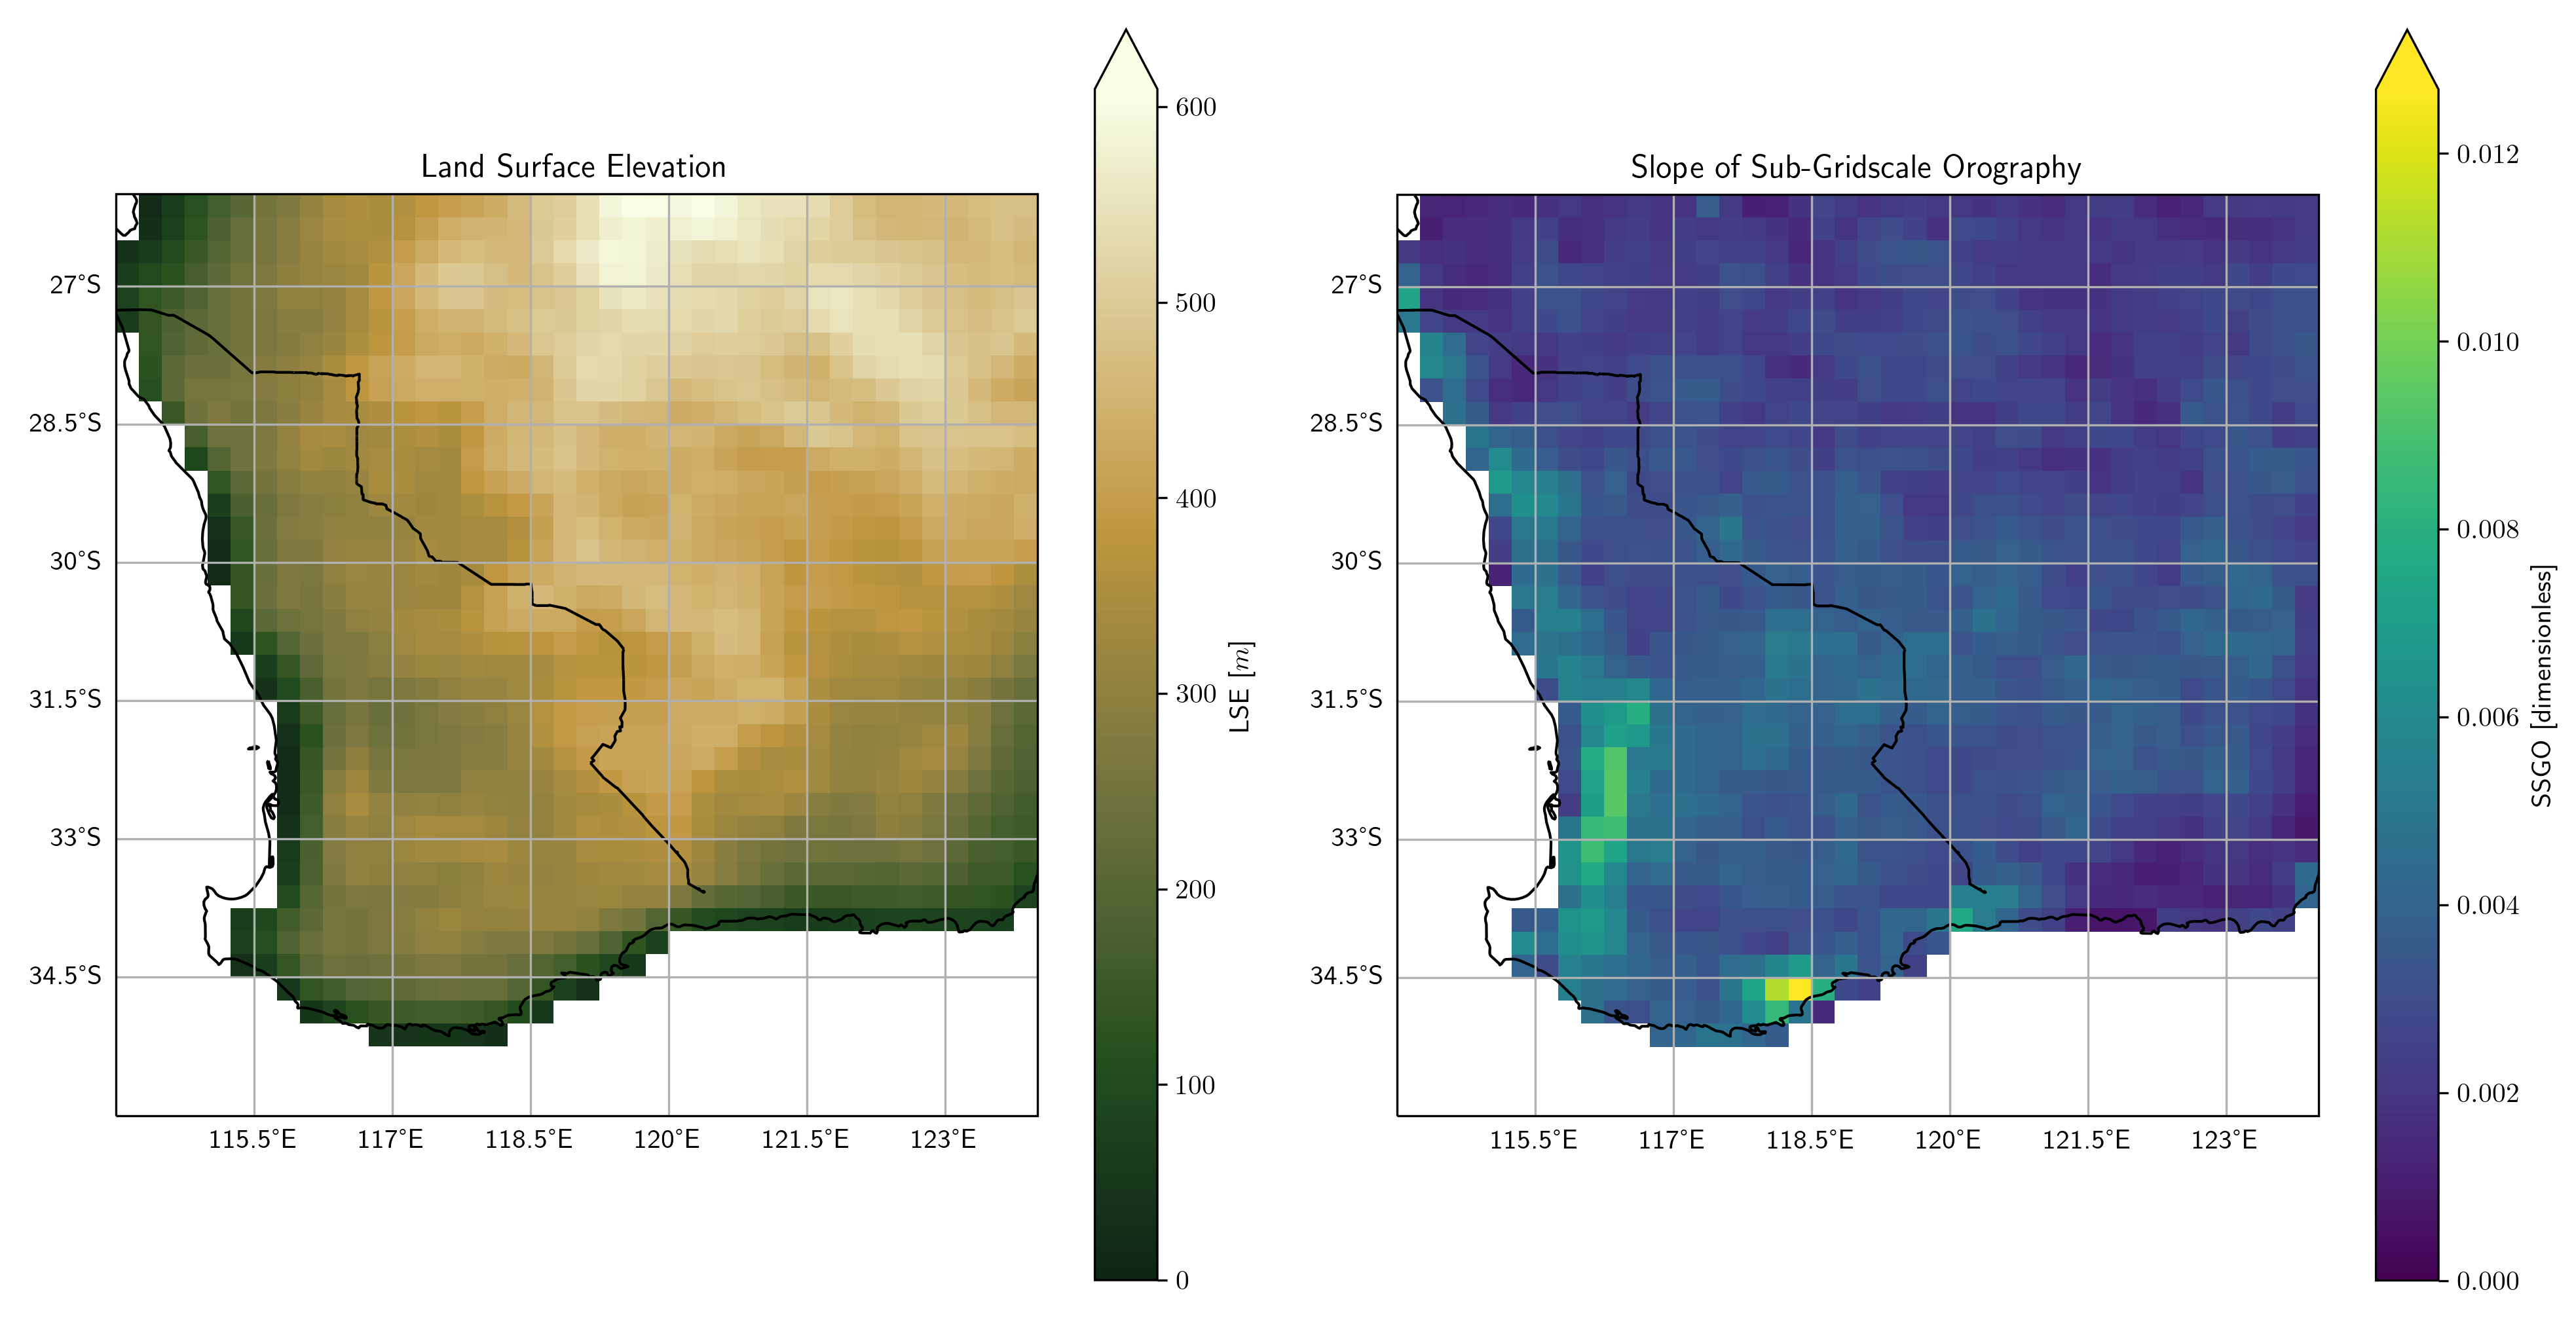
\includegraphics[width=0.9\textwidth]{wa_orog.png}
	\caption[Orography for WA focus region]{\acf{LSE} (left) and \acf{SSGO} (right) for the \ac{WA} focus region.}
	\label{fig:wa_orog}
\end{figure}

\section{Diurnal comparison for January mean}
\label{sec:comp_diurnal}

\subsection{VIEC delineation along fence}

\ac{VIEC} mean values computed over January displayed a marked distinction across the \acf{SBFWA}, with more strongly negative values on the native side of the fence during both the day and night (see Figure~\ref{fig:wa_jan_comb_1}).\footnote{The following results are also observed to varying degrees for the months of February, October, November and December, but we present January because this month displays these trends most distinctly.} During daytime, this also marks the distinction between positive \ac{VIEC} values on the agricultural side and negative values on the native side. Negative $\ac{VIEC}$ values indicate a greater prevalence for upwards air movement (kinetic energy converted into gravitational potential energy), while positive values indicate the opposite.\footnote{There are better variables than \ac{VIEC} in the ERA5 dataset to analyse upwards and downwards air movement since \ac{VIEC} lumps internal and gravitational potential energy together, but these other variables were not included in the original analysis and time constraints in this project did not allow for modification of the methodology. See Section~\ref{ssec:era5_improve}.}

\begin{figure}[!ht]
	\centering
	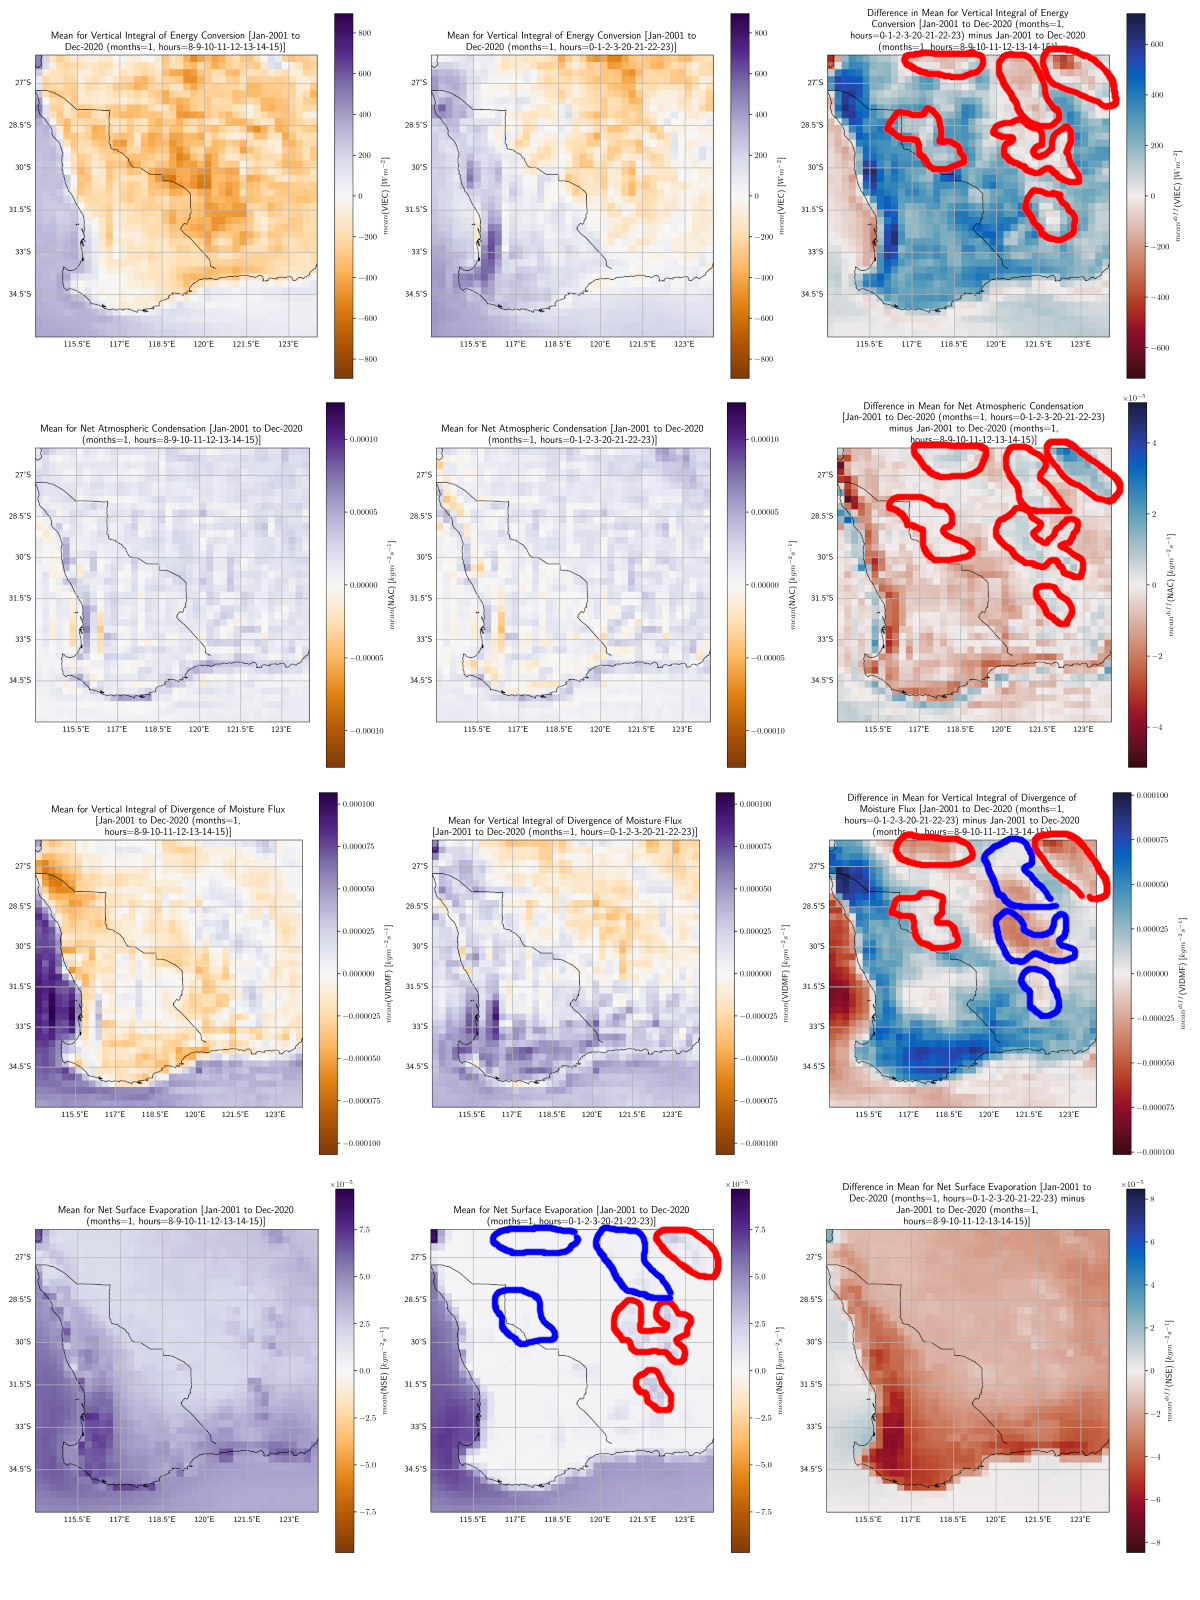
\includegraphics[width=0.9\textwidth]{wa_jan_comb_1.png}
	\caption[January means for selected variables 1]{January mean daytime and nighttime values for \acs{VIEC}, \acs{NAC}, \acs{VIDMF} and \acs{NSE}. Red markings indicate selected areas which are distinct from background trends. Blue markings indicate areas where such a distinction did not exist, but did exist for \acs{VIEC}.}
	\label{fig:wa_jan_comb_1}
\end{figure}

The large-scale patterns observed for \ac{VIEC}$^{diff}$ in arid \ac{WA} are mostly a reflection of warmer temperatures during daytime, and warmer temperatures on the native side due to thermal retention and lower albedo of native vegetation compared to bare agricultural soil in January. Evidence for this is a remarkable large-scale spatial correlation between \ac{T2}, \ac{MSLP} and \ac{VIEC} for all months of the year (not shown, but January results are displayed in Figure~\ref{fig:wa_jan_comb_2}). This suggests that the large-scale tendencies for vertical air mass movements in inland areas\footnote{Coastal effects are treated separately in Section~\ref{sec:comp_seasonal_1400}.} are driven by surface heating, in accordance with standard theory.

\begin{figure}[!ht]
	\centering
	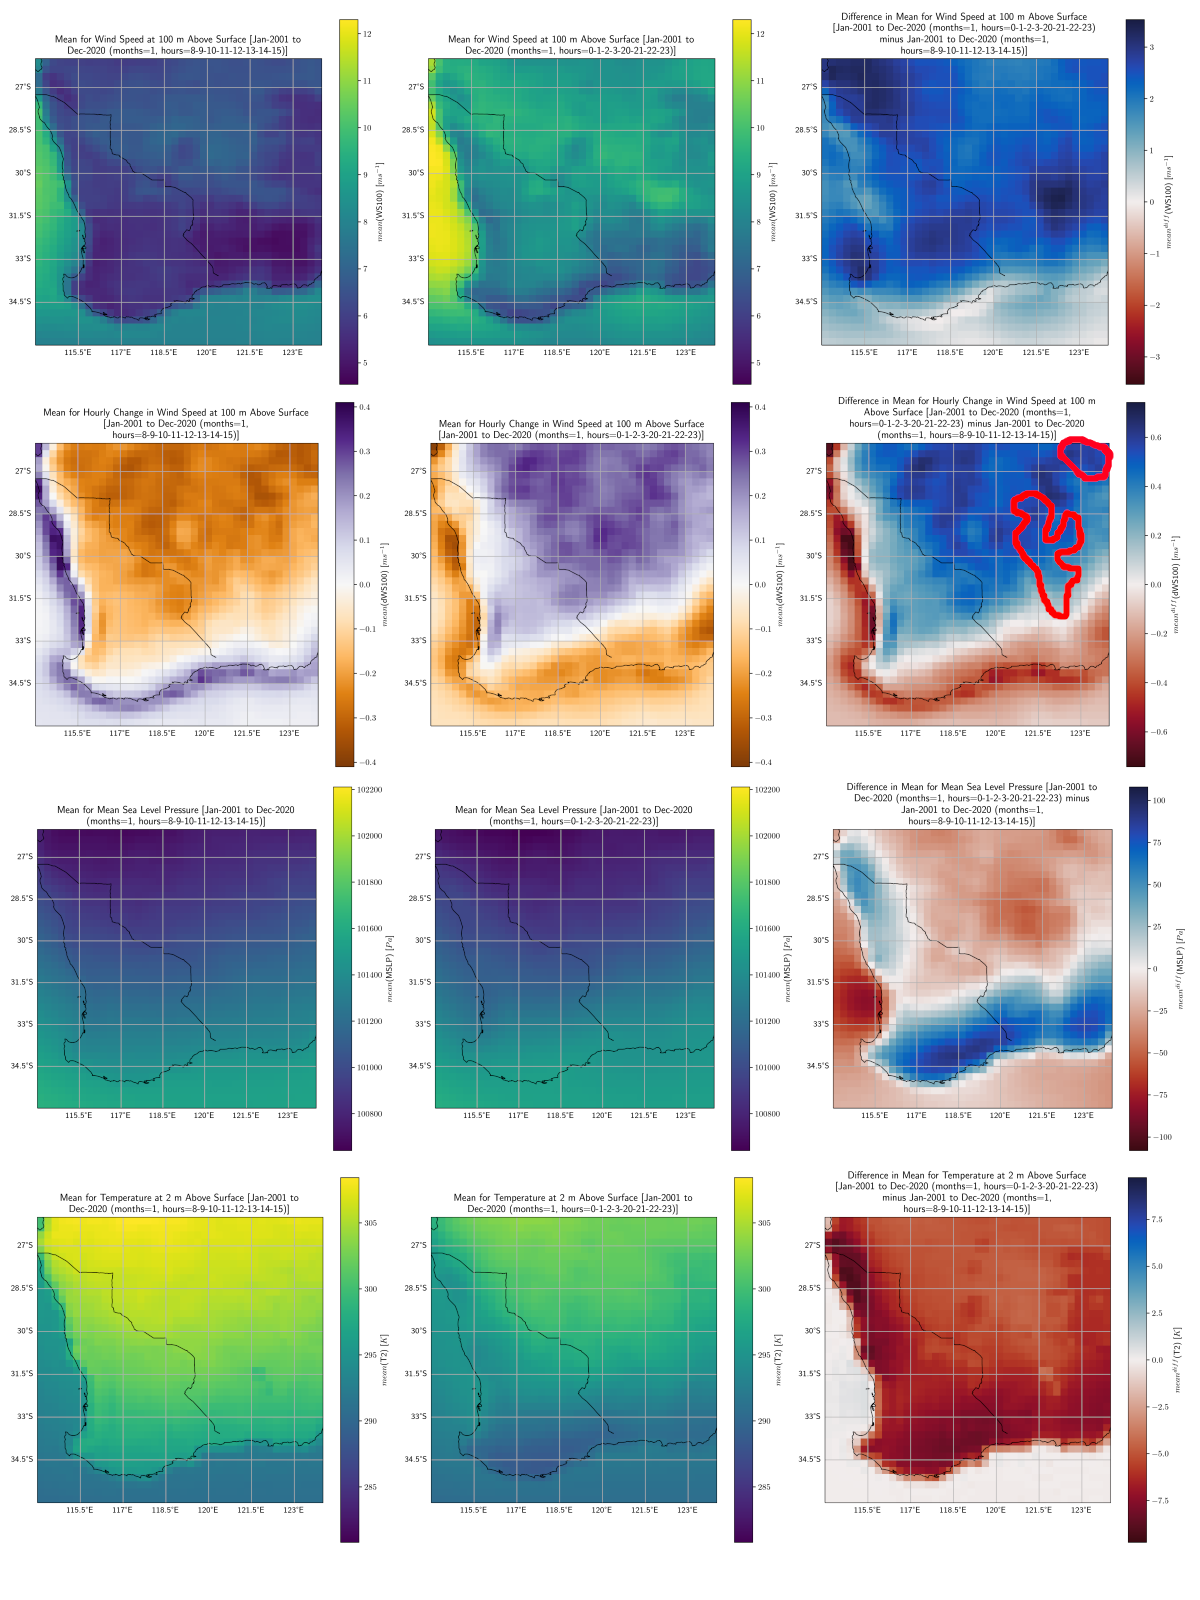
\includegraphics[width=0.9\textwidth]{wa_jan_comb_2.png}
	\caption[January means for selected variables 2]{January mean daytime and nighttime values for \acs{WS100}, \acs{dWS100}, \acs{MSLP} and \acs{T2}. Red markings indicate selected areas for \acs{dWS100} which are distinct from background trends but which deviate from orographic spatial patterns.}
	\label{fig:wa_jan_comb_2}
\end{figure}

\subsection{Localised anomalies}

However, there are local-scale features which act contrary to this background trend. These are highlighted with red markings in Figure~\ref{fig:wa_jan_comb_1}.\footnote{The use of coloured markings with a thick outline somewhat distorts perception of these features. For an unmarked version of the figure, see Appendix~\ref{sec:unmarked}.} In these areas, \ac{VIEC} becomes increasingly negative (air movements are increasingly upwards directed) from daytime to nighttime despite the decrease in temperature, and there did not appear to be any localised anomalies in \ac{T2} which could explain this (see Figure~\ref{fig:wa_jan_comb_2}).

Interestingly, these \ac{VIEC}$^{diff}$ anomalies correspond to localised areas of positive \ac{NAC}$^{diff}$ (see Figure~\ref{fig:wa_jan_comb_1}). Given the suspected role of \ac{CIAD}, we turn to the question of whether this correlation primarily reflects a chance convergence of winds manifesting stronger upwards air movements which was then conducive towards cloud formation, or whether the actual condensation itself was responsible for the strengthening vertical motions.

\subsection{Contribution from lake evaporation}

At least a few of these anomalies can be attributed to evaporation from ephemeral lakes\footnote{Although ephemeral, use of Google Earth satellite images confirms that these lakes contained water for all December months within the study period (and the water is presumably still there by January).}, which calls into question how relevant chance wind convergence would be on top of this. The lakes display a relatively low magnitude of evaporation decrease going from daytime to nighttime temperatures. This can be seen in the difference plot (right column) for \ac{NSE} in Figure~\ref{fig:wa_jan_comb_1} but for visual clarity, these lakes were marked in red for the nighttime plot (middle column) instead.

Furthermore, given the low magnitude of \ac{NSE} over these lakes relative to background trends, we would have expected increased water vapour \textit{divergence} via diffusion (positive \acs{VIDMF}$^{diff}$). But instead, what we observe is that these lakes correspond to areas of \textit{negative} \acs{VIDMF}$^{diff}$ (indicating increased water vapour \textit{convergence}). Given it is unlikely for a chance convergence of winds to coincidentally conform to the extents of the lakes, this flags the possibility of \ac{CIAD} as to our knowledge there has been no other proposed mechanism which would explain this anomaly. That is, continued evaporation combined with cooler temperatures during night time leads to increased atmospheric condensation, and under this may form a localised area of low pressure which advects air and moisture towards itself for sustenance.

\subsection{Implications for surface wind resource} 

In studying implications for wind energy generation, we turn towards 100 m wind speed (\acs{WS100}) as well as the \textit{hourly change} in 100 m wind speed (\acs{dWS100}). The latter allows us to analyse effects upon \acs{WS100} which may be slight and difficult to visually identify from a plot of \ac{WS100} itself since the signal is dominated by synoptic effects.

\subsubsection{WS100 higher on native side of fence}

Despite lower roughness on the agricultural side of the fence in January (when there is no crop and often bare soil), \ac{WS100} is higher on the native side of the fence and shows some signs of being delineated along the fence itself. This is likely a reflection of surface air pressure differences arising from temperature differences (see Figure~\ref{fig:wa_jan_comb_2} left and middle columns; note how the fence delineations for \ac{WS100}, \ac{MSLP} and \ac{T2} do not hold along the southern part of the region from 34.5$^\circ$S to 31.5$^\circ$S). Given that results for \ac{T2} shows a clear demarcation along the fence in Figure~\ref{fig:wa_jan_comb_2}, it then follows that wind speed variations beyond the effect of surface roughness can in part be attributed to the type of vegetation cover. Future changes to vegetation cover (such as eastward agricultural expansion, or change in crops being grown) which cause a decrease in temperatures may possibly reduce wind speeds (and the converse for increases in temperature).

\subsubsection{Anomaly for diurnal difference in MSLP on native side of fence}

\paragraph{Decrease in pressure despite convergence of mass and decrease in temperature}

Although the spatial pattern observed for \ac{MSLP}$^{diff}$ is similar to that of \ac{T2}$^{diff}$ in Figure~\ref{fig:wa_jan_comb_2}, a large area of the focus region (mostly on the native side of the fence) sees a \textit{decrease} in surface pressure going from day to night despite a decrease in temperature. So mass flux directed away from the surface of this area (i.e.\ decreasing surface pressure) does not appear to be caused by surface temperature changes inducing \textit{upwards} air movement. Nor does it appear to be caused by \textit{outwards} (horizontal) mass transport given that much of this area displays increased moisture \textit{convergence} (negative \acs{VIDMF}$^{diff}$) in Figure~\ref{fig:wa_jan_comb_1} (in turn implicating increasing \textit{convergence} of winds and air mass in general).

\paragraph{Possible explanations}

The remaining explanations are either that there is some climate feature in the upper atmosphere or outside of this focus region or which interacts with the surface of this focus region to produce a reduction of pressure towards nighttime, or that the reduction in surface pressure actually arises from a drop in air density as gaseous water condenses out as liquid.

The latter appears to only be mildly supported by the \ac{NAC} results in Figure~\ref{fig:wa_jan_comb_1}. An increase of condensation only occurs in certain parts of the area where there is negative \ac{MSLP}$^{diff}$, and these parts do correlate with especially negative \ac{MSLP}$^{diff}$ values, but it is not clear whether these distributed localisations of condensation can produce the area-scale effect seen for \ac{MSLP}$^{diff}$. However, it should be noted that much of the patchiness observed in \ac{NAC} could possibly result from the fact that \ac{NAC} is a hybrid value derived a mixture of instantaneous and accumulated \ac{ERA5} variables (see Appendix~\ref{sec:nac_derive}).

\paragraph{Possible implications for surface wind}

If it is indeed the case that atmospheric condensation is responsible for the surface pressure drop and hence increase in wind speeds, then this is yet another mechanism by which the surface wind resource depends on land cover, given results by \citep{lyons2002, ray2003} which clearly demonstrates that land cover modulates cloud formation preferences (also see Section~\ref{ssec:native_nac}).

\subsubsection{Anomalies in dWS100}

\paragraph{dWS100 correlated with LSE, VIEC and NAC}

The spatial pattern observed for \acs{dWS100} corresponds mostly to the \ac{LSE} displayed in Figure~\ref{fig:wa_orog}. Higher elevations are correlated with more negative d\ac{WS100} values during the daytime, more positive values during nighttime, and hence a greater magnitude of increase from day to night. Selected areas which display the opposite trends are highlighted with red markings in Figure~\ref{fig:wa_jan_comb_2}.\footnote{For an undistorted view, see the figure without markings in Appendix~\ref{sec:unmarked}.}

Interestingly, these areas correspond with the lakes identified earlier, and actually show an especially positive value for \acs{dWS100}$^{diff}$ (strengthening of winds). A more negative \ac{VIEC}$^{diff}$ (less conversion of internal and gravitational potential energy to kinetic) in these areas should imply a more negative \acs{dWS100}$^{diff}$ (weakening of winds) all other things equal, so it is not clear what is causing this anomaly. One possibility is that convection associated with increased \ac{NAC} (cloud formation) in these areas at nighttime lead to favourable energy exchanges between the boundary layer and free atmosphere, and a reversal of this effect in the daytime manifests as a greater decrease in wind speed.

\paragraph{Possible implications for surface wind}

If it can be shown that positive \ac{NAC}$^{diff}$ consistently correlates with especially positive \ac{dWS100}$^{diff}$, then land cover is again implicated through land cover modulation of cloud formation, with the effect that native vegetation induces a greater ramp rate in wind speeds in summer (when clouds preferentially form over the native side of the fence).

\section{Seasonal comparison for 1400 mean}
\label{sec:comp_seasonal_1400}

\subsection{Seasonal difference in MLAI}

Figure~\ref{fig:wa_lai_seasonal} displays a comparison for the \acl{MLAI} between the months of \ac{JJA} and \ac{DJF}. Native vegetation on the east of the \ac{SBFWA} show negligible differences. There is a significant loss in \ac{MLAI} towards the \ac{DJF} months as the wheat and barley crops which were grown from May to November are harvested in November \citep{lyons1996}. The extents of the \ac{MLAI} loss correspond well with the Wheat Belt region of Western Australia (see Figure~\ref{fig:lc_wa}). Slight (relative to \ac{JJA} base value) greening appears to occur in the coastal Jarrah forests through the spring and summer months.

\begin{figure}[!ht]
	\centering
	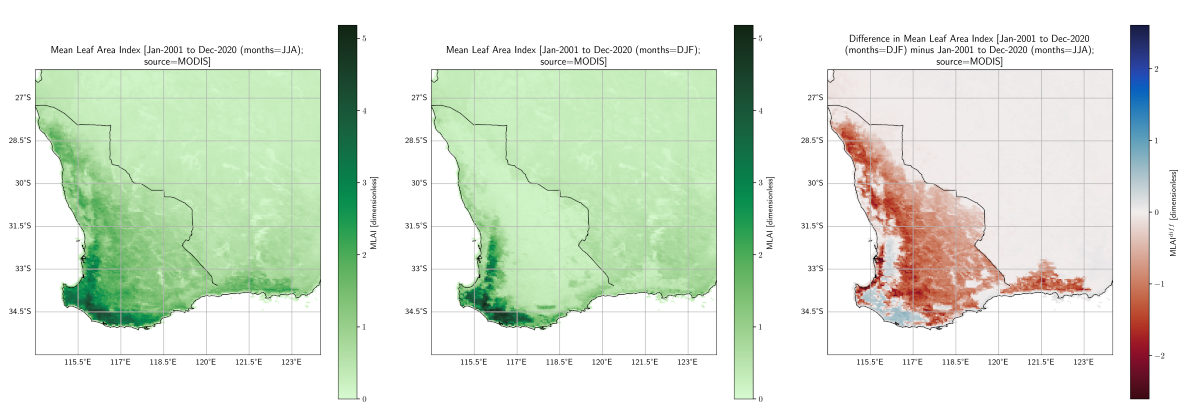
\includegraphics[width=0.9\textwidth]{wa_lai_seasonal.png}
	\caption[MLAI seasonal comparison for WA focus region]{\ac{MLAI} computed over \acs{JJA} and \acs{DJF} (left and middle), as well as the difference in these values between the two seasons (right).}
	\label{fig:wa_lai_seasonal}
\end{figure}

\subsection{Correlation between VIEC and NAC}

\ac{VIEC} mean values computed over 1400 \ac{LT} display a remarkable spatial correlation with that of \ac{NAC}. This is especially apparent near the coast for \ac{JJA} means, and in general for the difference plots between \ac{JJA} and \ac{DJF} (leftmost and rightmost columns in Figure~\ref{fig:wa_14_comb_1} respectively). More positive \ac{NAC} and \ac{NAC}$^{diff}$ values are correlated with more negative \ac{VIEC} and \ac{VIEC} $^{diff}$ values respectively. \ac{T2}$^{diff}$ (see Figure~\ref{fig:wa_14_comb_2}) shows a relatively uniform pattern and is consistent with the large-scale trend in \ac{VIEC} $^{diff}$ (warmer air tends to rise more), but it does not capture any of the smaller-scale trends that \ac{NAC}$^{diff}$ does.

\begin{figure}[!htp]
	\centering
	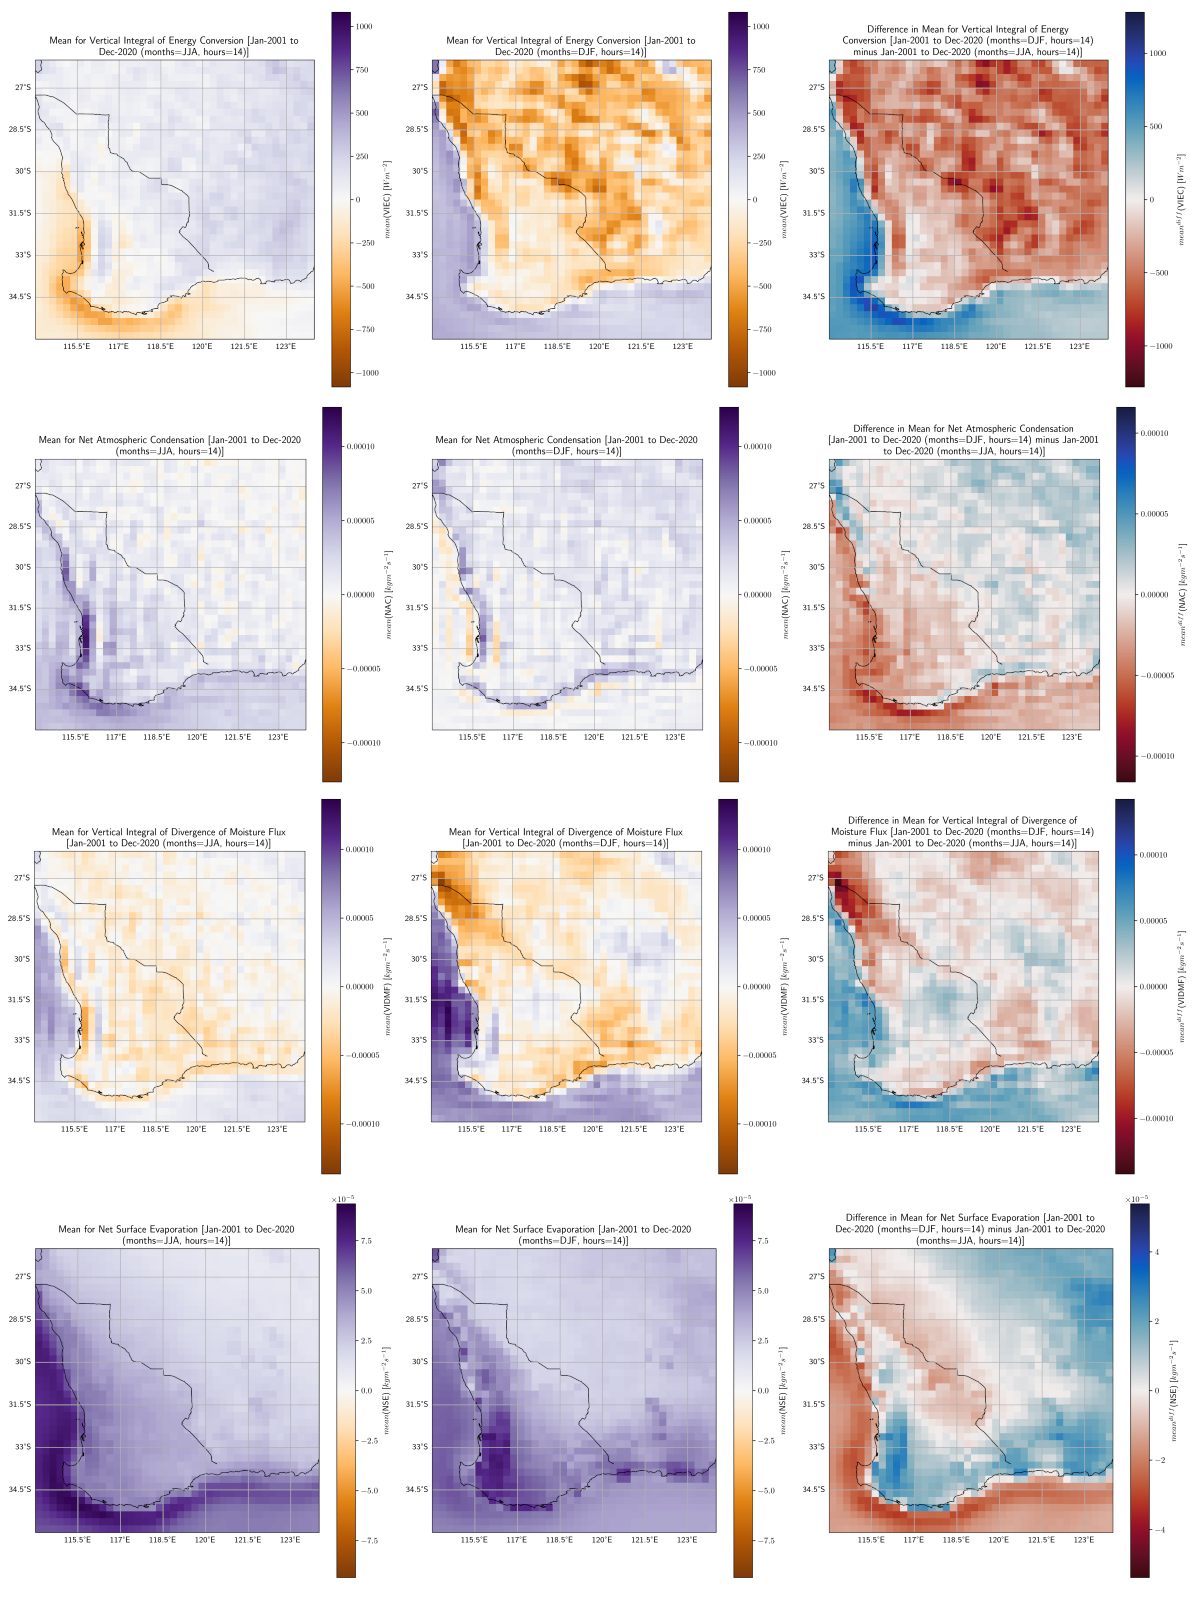
\includegraphics[width=0.9\textwidth]{wa_14_comb_1.png}
	\caption[1400 means for selected variables 1]{1400 mean \acs{JJA} and \acs{DJF} values for \acs{VIEC}, \acs{NAC}, \acs{VIDMF} and \acs{NSE}.}
	\label{fig:wa_14_comb_1}
\end{figure}

\begin{figure}[!htp]
	\centering
	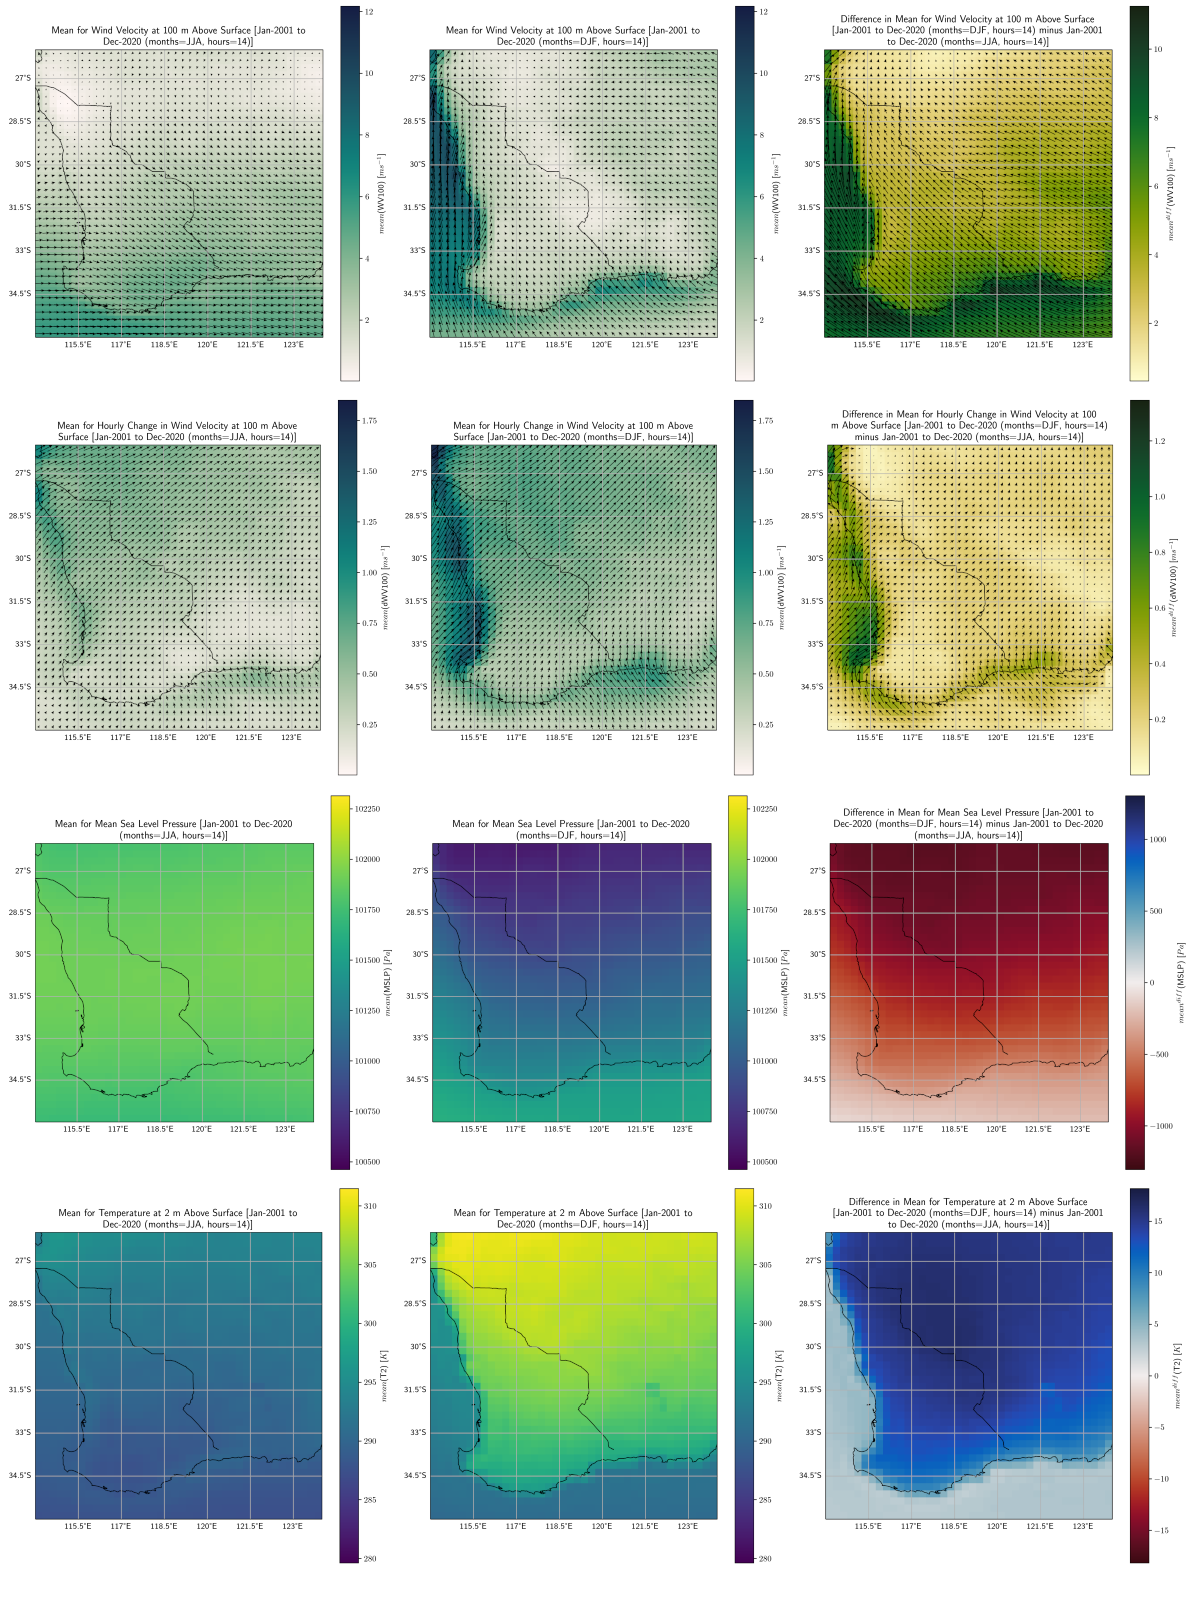
\includegraphics[width=0.9\textwidth]{wa_14_comb_2.png}
	\caption[1400 means for selected variables 2]{1400 mean \acs{JJA} and \acs{DJF} values for \acs{WV100}, \acs{dWV100}, \acs{MSLP} and \acs{T2}.}
	\label{fig:wa_14_comb_2}
\end{figure}

We choose to display results for 1400 \ac{LT} here because results for this hour are most distinct, but the following is actually more or less observed for all hours of the day in the hourly means analysis and all months of the year in the monthly means analysis (not shown):
\begin{itemize}
	\item For both \ac{JJA} and \ac{DJF} results, we observe that on the native side of the fence, most areas of negative \ac{VIDMF}$^{diff}$ (increased moisture \textit{convergence}) correlate with areas of positive \ac{NSE}$^{diff}$ (increased evaporation) but positive \ac{NAC}, contrary to what is expected from diffusion but consistent with \ac{CIAD}.
	\item None of the variables from which \ac{NAC} is derived display similar local-scale spatial variations to \ac{VIEC} across most of the focus region (\ac{VIDMF} and \ac{NSE} for 1400 are displayed in Figure~\ref{fig:wa_14_comb_1}, \ac{TCWV} not shown at all). Only \ac{NAC} itself is similar to \ac{VIEC}.\footnote{Exceptions occur for hours 0500-0700 \ac{LT} and 1700-1900 \ac{LT} due to data artefacts in \ac{ERA5}, but this should not affect the conclusions. See Appendix~\ref{sec:artefact} for discussion.}
	\item The concentrated band of negative \ac{VIEC} and positive \ac{NAC} means along the southwestern coastline for \ac{JJA} is present regardless of whether the band is upwind or downwind of the coastline, and whether the temperature gradients are producing a land or sea breeze (see \ac{T2} and \ac{dWV100} in Figure~\ref{fig:wa_14_comb_2} for 1400 \ac{LT} results).
\end{itemize}

The final point indicates that coastal orography and differential heating are unlikely to be responsible for the concentrated band along the southwestern coastline. And these points together conspire to heavily implicate the possibility of \ac{CIAD}.

\subsection{The role of coastal geography}

One way in which negative \ac{VIEC} (rising air) could theoretically be concentrated along the coastline is if low-lying oceanic winds experience a sudden change in surface elevation and are deflected upwards from coastal cliffs and urban structures. But this does not explain why the observed bands in Figure~\ref{fig:wa_14_comb_1} extends out into the oceans, nor why the band is observed on the southernmost part of this region (around 35$^\circ$S) where winds are blowing from relatively high terrestrial ground to relatively low ocean surface (see \ac{WV100} in Figure~\ref{fig:wa_14_comb_2}). Furthermore, much stronger winds are blowing onshore during the \ac{DJF} months yet this coastal band is not observed for these months (compare \ac{VIEC} in Figure~\ref{fig:wa_14_comb_1} with \ac{WV100} in Figure~\ref{fig:wa_14_comb_2}). So it seems extremely unlikely that coastal orography is the cause.

\subsection{The role of coastal differential heating}

Another way in which negative \ac{VIEC} (rising air) could theoretically be concentrated along the coastline is if a localised pressure gradient (arising from a temperature gradient) along the coastline adverse to the wind direction caused a bunching up of mass such that air had to be directed upwards. But results indicate the presence of this band regardless of the strength and direction of the coastline temperature gradient relative to prevailing winds. For the case of 1400 \ac{LT}, Figure~\ref{fig:wa_14_comb_2} displays a negligible coastal pressure gradient, temperature gradient and magnitude of \ac{dWV100} in \ac{JJA}, yet the band exists for these months but not \ac{DJF} where these parameters are much more significant. So it also seems highly unlikely that differential heating is the cause.

Although Figure~\ref{fig:wa_14_comb_2} displays a negligible coastal gradient in \textit{air} temperature for \ac{JJA} at 1400 \ac{LT}, the Leeuwin (Ocean) Current during these months actually brings about a significant increase in \ac{SST} for the continental shelf waters \citep{berthot1997}. This can be seen in Figure~\ref{fig:wa_14_comb_1}, where offshore evaporation is significantly higher in \ac{JJA} than \ac{DJF} despite lower solar irradiance.

\subsection{The role of coastal condensation}
\label{ssec:coastal_cond}

\subsubsection{Atmospheric condensation as cause for convective initiation}

\paragraph{Summary of conclusions from seasonal comparison thus far}

In summary, the coastal concentration of negative \ac{VIEC} (upwards air movements) occurs in continental shelf waters where \textit{air} temperature is comparable to that on land, but where \textit{water} temperatures are higher than that of air due to the winter presence of the Leeuwin Current. There is additional atmospheric moisture from the warmer waters which contributes to air buoyancy but analysis of \ac{CAPE} values reveals no coastal concentration whatsoever (not shown).\footnote{This is in spite of the fact that \ac{CAPE} in the \ac{ERA5} dataset is known to occasionally give unrealistically high values \citep{ecmwf}.} So having ruled out mechanical deflection of winds from coastal geography, localised pressurisation from coastal differential heating, higher offshore \textit{air} temperatures leading to upwards thermal expansion, and additional air buoyancy from increased atmospheric moisture, \ac{CIAD} is to our knowledge the only proposed mechanism consistent with the results.

\paragraph{Direction of causation}

In the \ac{CIAD} picture, additional winter atmospheric moisture from the Leeuwin Current is conducive towards coastal cloud formation, and it is this atmospheric condensation (positive \ac{NAC}) which initiates convection and subsequent uplift of air (negative \ac{VIEC}). That is, the direction of causation for \textit{initiation} of local circulations is from condensation to convection. In the ensuing circulation, the direction of causation is ill-defined as there is a positive feedback loop between the two. The circulation persists until the available moisture (latent energy) is unable to sustain the air motions.

\subsubsection{Interactions with temperature gradients and surface energy fluxes}
\label{ssec:nac_t2}

On top of this, there is the effect of coastal temperature gradients in determining the spatial distribution of atmospheric moisture available for condensation, and the effect of \ac{SSHF} inland in determining whether there is sufficient convective mixing for the \ac{BLH} to penetrate the \ac{LCL} for condensation to occur.

\paragraph{Consistency with JJA results}

Weaker winds from temperature gradients in \ac{JJA} compared to \ac{DJF} means the buildup of oceanic moisture along the coasts has a high condensation rate relative to moisture convergence flux to inland areas. For the 1400 \ac{LT} case, this is reflected in \ac{JJA} by low \ac{WV100} magnitude, low \ac{dWV100} magnitude and weak coastal \ac{T2} contrast in Figure~\ref{fig:wa_14_comb_2}, as well as a less positive \ac{VIDMF} offshore (west of the coastline) despite higher \ac{NSE} in Figure~\ref{fig:wa_14_comb_1}. The result is that \ac{VIEC} displays a similar band to \ac{NAC} along the coast. This is also supported by the fact that the negative \ac{VIEC} band is absent from around 29$^\circ$S to 27$^\circ$S, which coincides with where \ac{dWV100} is especially strong.

\paragraph{DJF results and flux of moisture convergence towards fence}

On the other hand, stronger winds from temperature gradients in \ac{DJF} imply the converse. The ratio of inland moisture flux transport to coastal condensation rate is relatively high (in part due to lower coastal moisture from absence of Leeuwin Current), so no coastal band of negative \ac{VIEC} is observed. Instead, there is increased condensation (relative to \ac{JJA}) on the native side of the fence, possibly due to higher \ac{SSHF}, and this is where negative \ac{VIEC} concentrates instead. This would seem to be supported by \ac{VIDMF} results which show for \ac{DJF} how moisture convergence (negative \ac{VIDMF}) moves inland ahead of moisture divergence (positive \ac{VIDMF}) as the day progresses, eventually reaching a point where convergence is concentrated on the native side of the fence (see Figure \ref{fig:wa_vidmf}).

\begin{figure}[!htp]
	\centering
	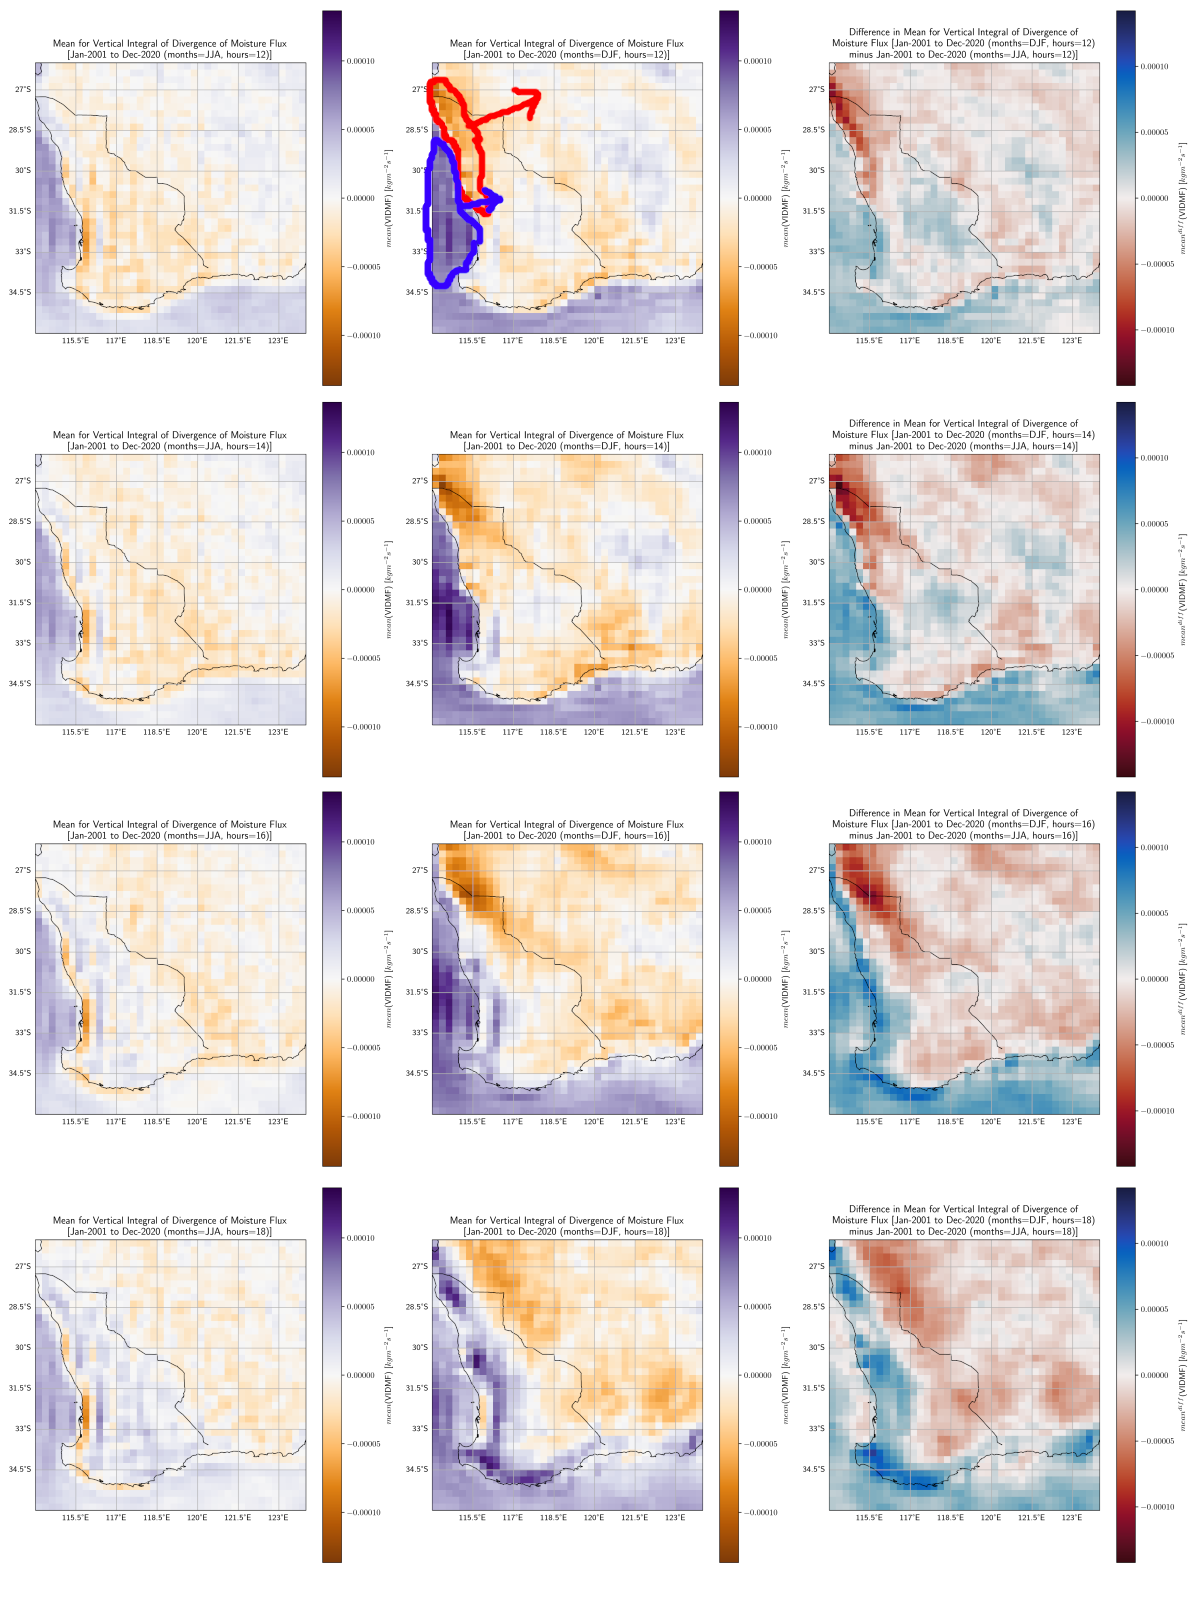
\includegraphics[width=0.9\textwidth]{wa_vidmf.png}
	\caption[1200-1800 means for VIDMF]{1200-1800 mean \acs{JJA} and \acs{DJF} values for \acs{VIDMF}. Red and blue markings illustrate how moisture convergence and divergence respectively is initially concentrated near the coastline then moves inland as the day progresses, eventually reaching a point where convergence is concentrated on the native side of the fence.}
	\label{fig:wa_vidmf}
\end{figure}

\subsection{Implications for surface wind resource} 
\label{ssec:implications}

\subsubsection{Effect on coastal breezes}

The replacement of native vegetation with annual crops, where there is irrigation in winter, bare cover after harvesting in summer, and lower albedo year round, has likely led to the lower surface temperatures observed on the western side of the \ac{SBFWA} year round. These lower temperatures were observed in the monthly means analysis for \ac{T2} (not shown) but can also be seen in Figure~\ref{fig:wa_14_comb_2} for the case of 1400 \ac{LT} in \ac{DJF}. Assuming that native vegetation cover which existed in the southwest region prior to agricultural clearing had similar temperatures to that currently observed on the native side of the fence, diurnal monthly means analysis (not shown) suggests that the agricultural clearing has led to:
\begin{itemize}
	\item For daytime during warmer months (Oct to Mar): a weakening of the sea breeze
	\item For nighttime during warmer months (Oct to Mar): a slight strengthening of the land breeze, with possibly a reversal from slight sea breeze to slight land breeze
	\item For daytime during cooler months (Apr to Sep): a slight strengthening of the land breeze, with possibly a reversal from slight sea breeze to slight land breeze
	\item For nighttime during cooler months (Apr to Sep): a very slight strengthening of the land breeze
\end{itemize}

\subsubsection{Inland drying and coastal flooding}

In all cases this points towards a loss in inland atmospheric moisture, and may partly explain the well documented loss of rainfall and water vapour in the southwest region \citep{gordon2003, narisma2003, pitman2004, junkermann2009}. To the extent that atmospheric moisture is oceanic in origin (as opposed to from plant transpiration), as is often the case given the coastal location and dry climate of this region, a corollary to reduced inland moisture flux is an increased flood risk from the coastal buildup of moisture.

\subsubsection{Possible exacerbation under CIAD}

The available evidence appears to support the \ac{CIAD} framework moreso than it does the notion that cloud formation is a passive byproduct of moist air masses rising (whether due to surface heating, orography or chance convergence of winds). This is unless there is some systematic error in the \ac{ERA5} dataset which we are not aware of and which just so happens to produce misleading results.

Assuming this isn't the case and also assuming that the \ac{CIAD} framework is valid, then beyond ocean-land temperature differences from native vegetation clearing there would have been an additional contribution from reduced atmospheric condensation. That is, the drop in air pressure which accompanies atmospheric condensation becomes less prevalent, so even less air and moisture is advected inland. And the result is further exacerbation to inland rainfall loss and coastal flood risk.

\subsubsection{How this affects wind energy operation}

\paragraph{Operational revenue and risk}

The strengthening and weakening of breezes has a direct impact on how much energy coastal wind farms are able to generate. Coastal breeze changes appear to only be slight except in the case of daytime during warmer months (Oct to Mar). These months also happen to be when energy demand from air conditioning is at its highest so all other things equal, this translates to a loss in wind generation revenue compared to if current agricultural cover was instead native vegetation cover. This is especially so since a weakening of the sea breeze also means less cool relief for the urban centre of Perth.

Coastal flooding also constitutes a tail risk for wind energy operation. There is obvious damage that can be done to both turbine structures as well as accompanying electrical infrastructure. Despite the context of continued climate change, such increases in risk might not yet be internalised within project costs. Failure to properly capture these risks may produce losses which deter future investment.

\paragraph{Future changes in land cover}

There is further risk embodied within uncertainty of what future land cover will be. Afforestation efforts are a real possibility given increasing environmental consciousness by the public. Changing geopolitical-economic conditions, climate and public favour may also give way to the growing of different crops (including summer crops) in this region. Continued agricultural expansion is another possibility. In all these cases, it matters what species of trees or crops are being grown and how, as this determines the subsequent surface energy fluxes, temperature, and roughness.

Large-scale coastal afforestation using eucalypts with low albedo and high \ac{SSHF}, for example, are likely to strengthen the summer daytime sea breeze due to higher coastal temperatures (but it is unclear how sustainable this will be without the appropriate matter flux feedbacks (e.g.\ water, nutrients) granted by appropriate biodiversity). The large-scale adoption of summer crops with irrigation on the other hand, is likely to weaken the summer daytime sea breeze due to lower inland temperatures.

\paragraph{Possible changes in turbulence and condensation hotspots}

If \ac{CIAD} is valid, then the previous comments apply even more so. This also implies that land cover determines the concentration and spatial distribution of turbulence from rising air masses (negative \ac{VIEC}) via atmospheric condensation (positive \ac{NAC}). This in turn can introduce fatigue to turbine components and complex wake effects which inhibit energy generation. On top of this, future mining activity may change condensation hotspots and hence circulation patterns via changes in lake geochemistry affecting \ac{CCN} production \citep{junkermann2009}.

\section{Seasonal comparison for MDP statistics}

\subsection{Likely influence of agriculture on VIKE}

\subsubsection{Delineation along fence}

Figure~\ref{fig:wa_stats_seasonal_1} displays a delineation along the \ac{SBFWA} for $range$(\acs{VIKE}) and $hour_{max}$(\acs{VIKE}) in \ac{JJA}. None of the other \ac{MDP} statistics for \ac{VIKE} displayed remarkable results, and this spatial pattern may just be a coincidence. But the \ac{JJA} value for $range$(\acs{VIEC}) shows not only a delineation along the fence, but also along the edges of the coastal forests (compare with Figure~\ref{fig:wa_lai_seasonal}). However, this can also be interpreted as a coastal effect extending inland which is unrelated to the forests (it is difficult to distinguish between these since the forest cover follows the shape of the coastline).

\begin{figure}[!htp]
	\centering
	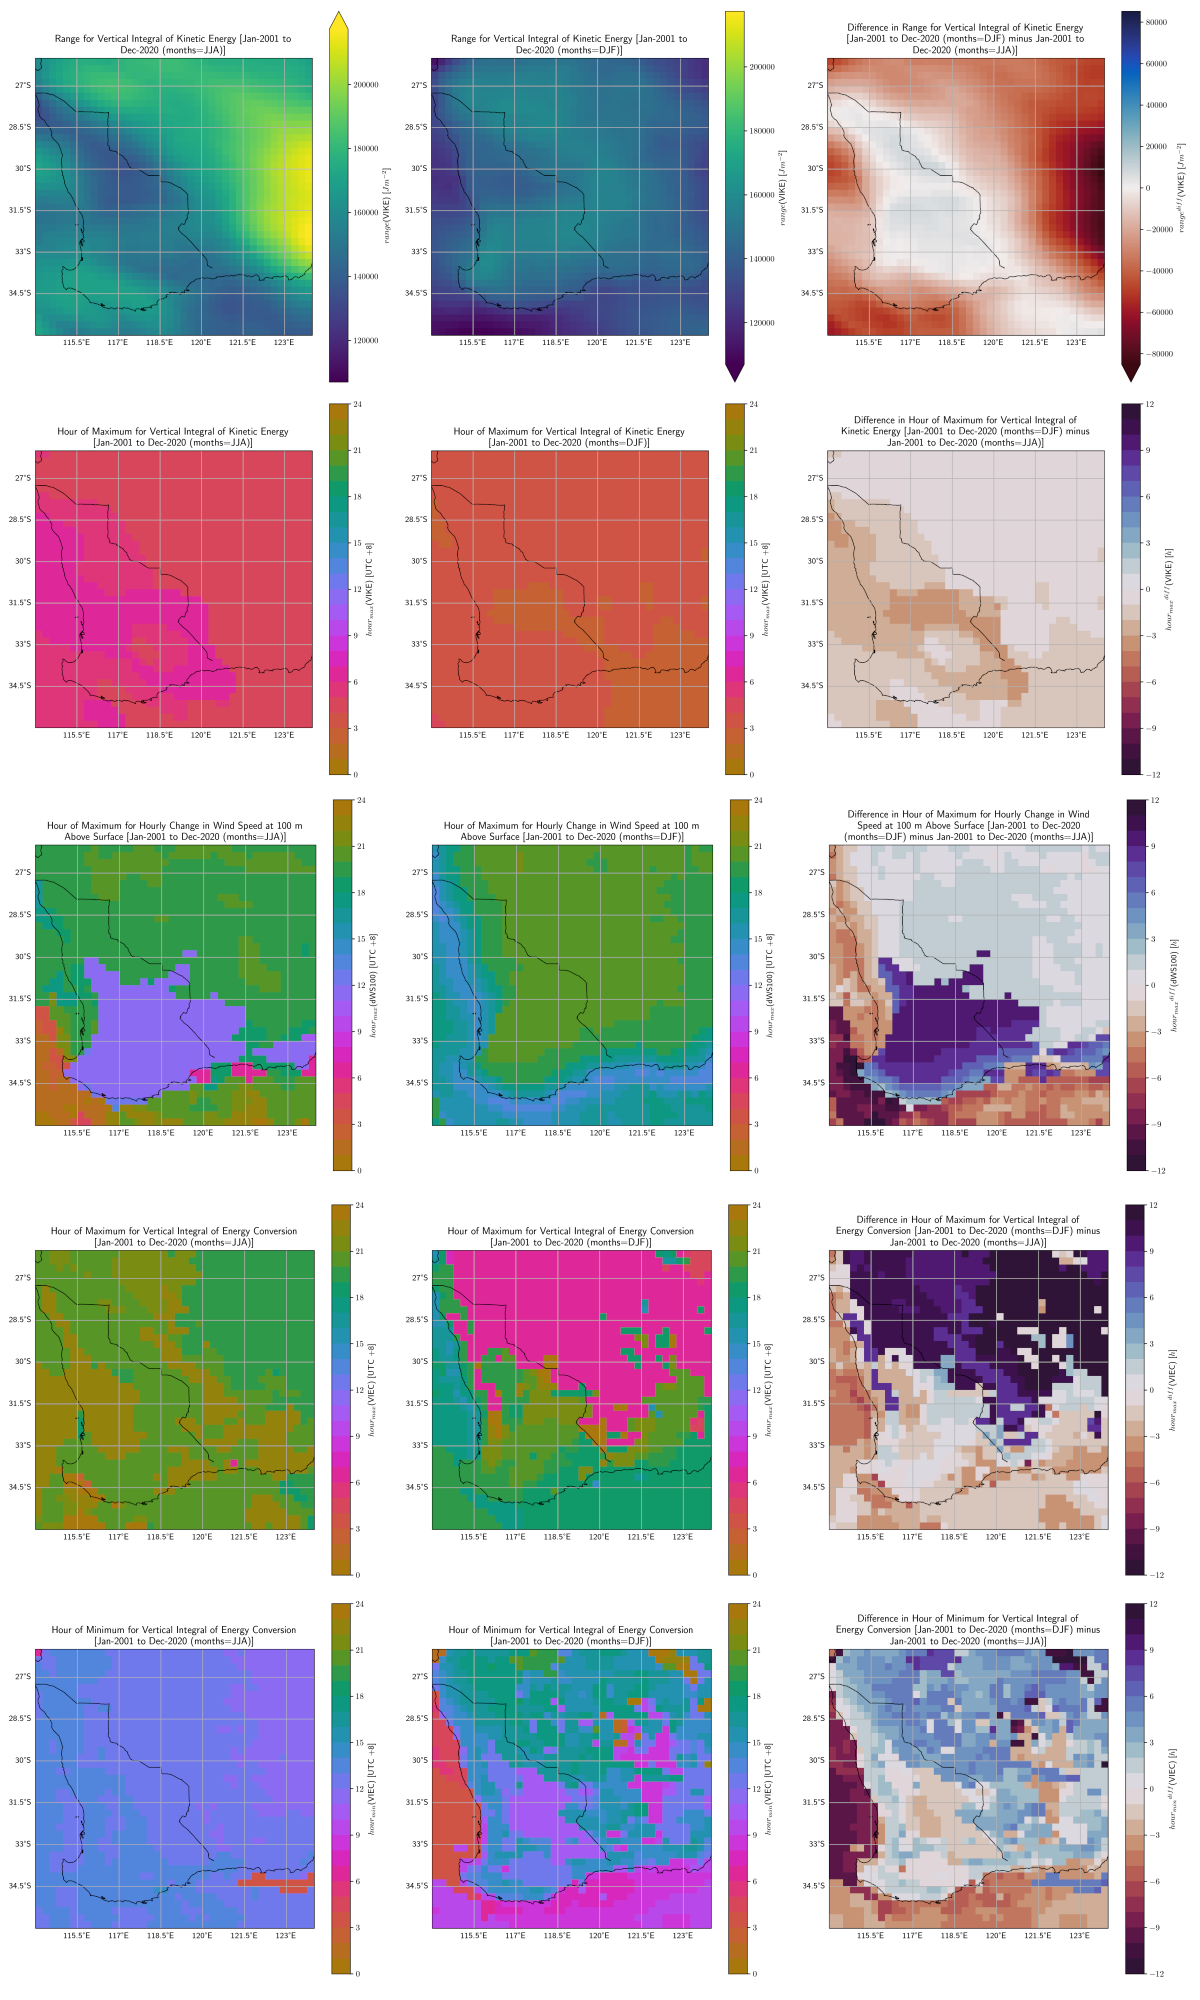
\includegraphics[width=0.75\textwidth]{wa_stats_seasonal_1.png}
	\caption[Selected MDP statistics with fence delineations]{Selected \ac{MDP} statistics (across various variables) which displayed delineations along the fence. Top to bottom: $range$(\acs{VIKE}), $hour_{max}$(\acs{VIKE}), $hour_{max}$(\acs{dWS100}), $hour_{max}$(\acs{VIEC}), $hour_{min}$(\acs{VIEC}).}
	\label{fig:wa_stats_seasonal_1}
\end{figure}

\subsubsection{Description of trends}

The \ac{JJA} values for \ac{VIKE} on the agricultural side show a smaller range, and an hour of maximum which is around two hours earlier. This is around the time of the morning boundary layer transition. \ac{VIKE} includes upper atmospheric air, so may be related to the surface via the boundary layer-free atmosphere interface. However, it is still unclear whether this is relevant and what is causing the observed spatial pattern. It is difficult to assess what effect cloud formation (which happens near the boundary layer-free atmosphere interface) might have, because \ac{NAC} is affected by assimilation cycle artefacts during these hours (see Appendix~\ref{sec:artefact}).

\subsubsection{Possible role of soil moisture}

Modelling by \citet{martius2021} suggests that soil moisture can have significant effects on the upper atmosphere. But to the extent that this is generally true of \acp{GCM}, the spatial pattern can also be interpreted as an artefact arising from sensitivities in the \ac{ECMWF} \ac{IFS} (which produces the \ac{ERA5} dataset). As \ac{VIKE} is a measure of \textit{horizontal} kinetic energy, this may affect the surface wind resource. But it is not clear how ($range$(\acs{WS100}) does \textit{not} show a similar pattern; not shown).

\subsection{Possible influence of agriculture on dWS100}

Figure~\ref{fig:wa_stats_seasonal_1} displays a somewhat marked distinction across the fence for $hour_{max}$(\acs{dWS100}) in \ac{JJA}. But the distinction does not sharply match the fence delineation. The results appear to suggest that wind speeds increase at the fastest rate around noon on the agricultural side and around the evening \ac{ABL} transition on the native side. $max$(\acs{dWS100}) displayed an increase from \ac{JJA} to \ac{DJF} over the entire region, with no obvious distinction across the fence (not shown). It is not known what is causing these results and whether this is reflecting an assimilation cycle artefact in \ac{ERA5} which we missed (see Appendix~\ref{sec:artefact}).

\subsection[Effect of native vegetation on VIEC diurnal phase]{Effect of native vegetation on phase of VIEC diurnal cycle}

\subsubsection{Minimum VIEC}

Figure~\ref{fig:wa_stats_seasonal_1} displays a delineation along the \ac{SBFWA} for $hour_{max}$(\acs{VIEC}) and $hour_{min}$(\acs{VIEC}) in \ac{DJF}. The bare agricultural cover in \ac{DJF} sees most negative \ac{VIEC} around noon, probably due to surface heating producing uplift of air. The native side sees most negative \ac{VIEC} (maximum uplift) at around the evening \ac{ABL} transition, well past the prime hours for solar heating. This is possibly associated with atmospheric condensation (in line with the \ac{CIAD} framework), but this is difficult to confirm due to assimilation cycle artefacts in \ac{NAC} during these hours (see Appendix~\ref{sec:artefact}).

\subsubsection{Maximum VIEC}

Interestingly, most positive \ac{VIEC} (minimum uplift) on the agricultural side also occurs around the evening \ac{ABL} transition. This indicates the possibility for atmospheric energy exchanges across the fence, where rising air on the native side spreads outwards then sinks on the agricultural side before returning to the native side. This would be consistent with the flux of atmospheric moisture convergence towards the native side of the fence noted in Section~\ref{ssec:nac_t2}.

\subsubsection{Divergent wind changes during evening}

Hourly means analysis for \ac{WV100} in \ac{DJF} reveals that surface winds have a southeasterly to southwesterly direction around this time (see Figure~\ref{fig:wa_19_comb}), and is perpendicular to the fence only in the northern part of the fence, so any fence breezes which exist appear to be weak relative to the synoptic background. Nevertheless, there is evidence for a fence breeze effect in \ac{dWV100}, as strengthening of the southeasterly winds near the southern part of the region (marked by red arrows in Figure~\ref{fig:wa_19_comb}) is biased towards divergent directions (towards both the coast \textit{and} the fence). Similar results appear for hourly means analysis from 1600-2000 \ac{LT} (not shown).

\begin{figure}[!htp]
	\centering
	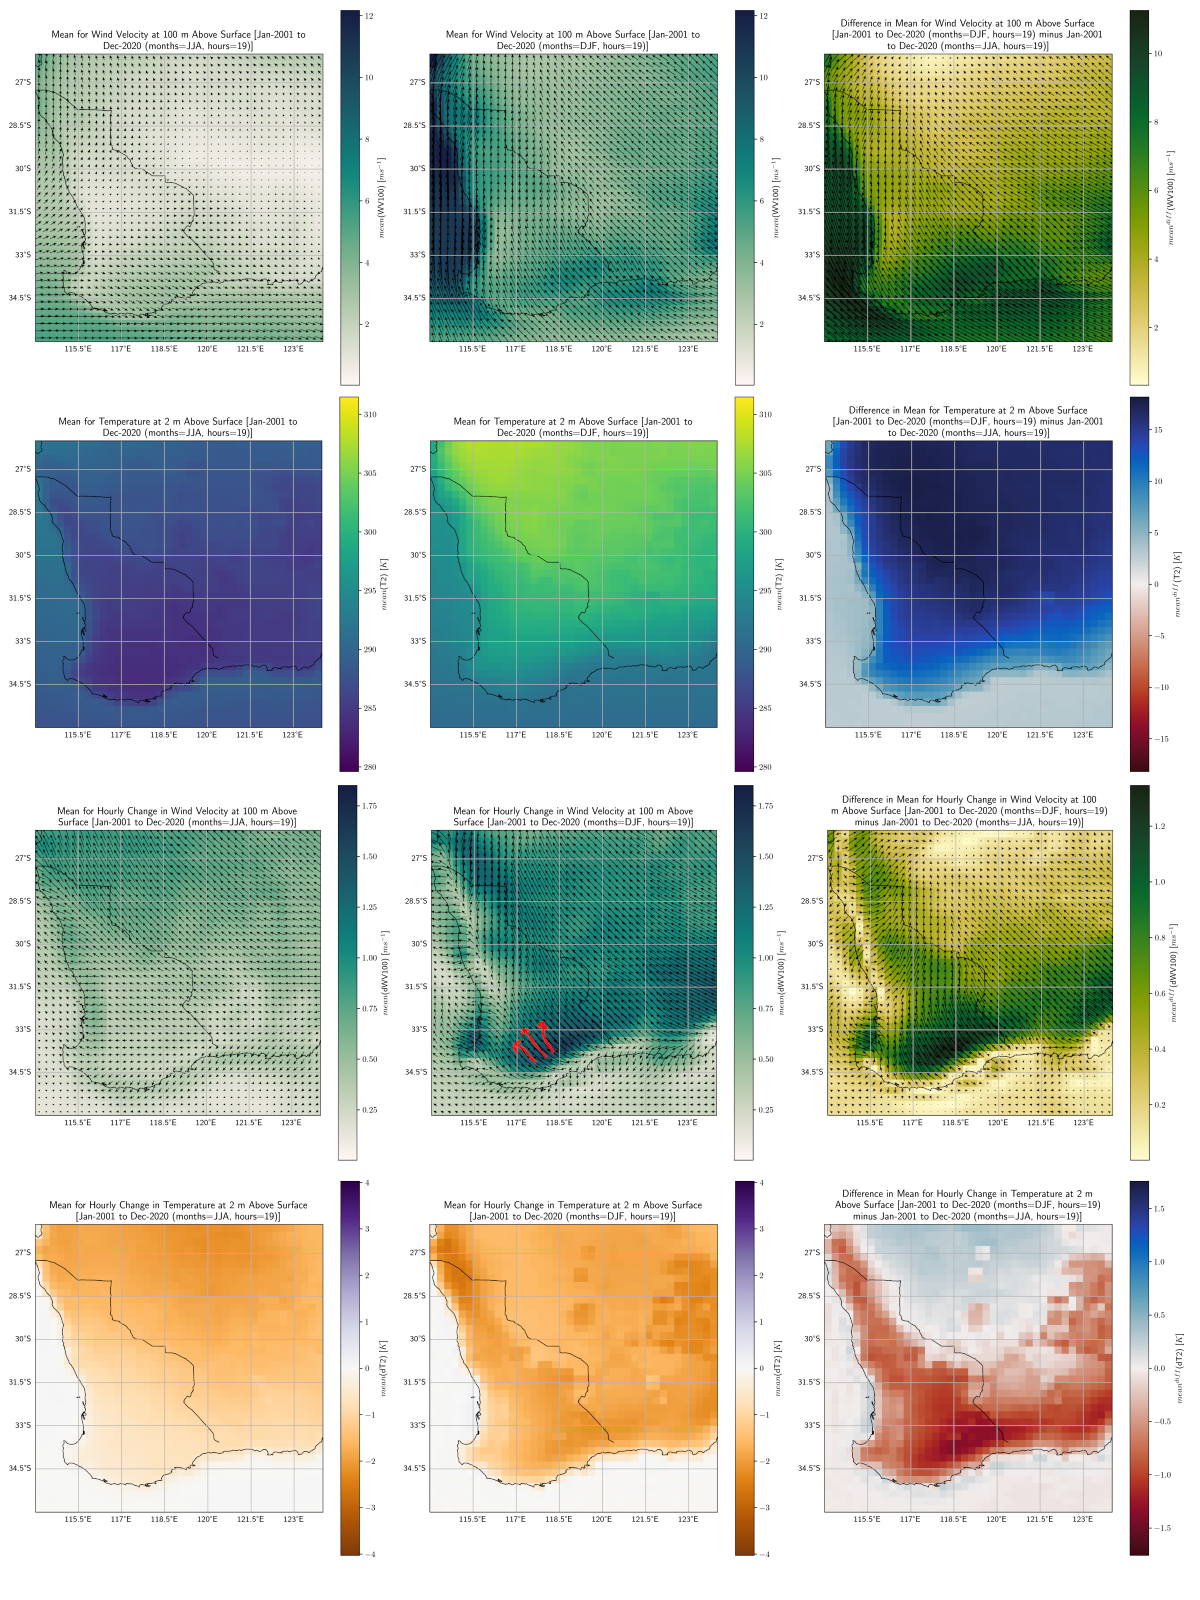
\includegraphics[width=0.9\textwidth]{wa_19_comb.png}
	\caption[Divergent wind changes during evening]{1900 mean \ac{JJA} and \ac{DJF} values for \acs{WV100}, \acs{T2}, \acs{dWV100} and \acs{dT2}. Red arrows (exaggerated) highlight the divergence in hourly wind changes. Magnitude of \ac{dWV100} near northern part of fence is higher than nearby coast despite weaker contrast in \ac{dT2}.}
	\label{fig:wa_19_comb}
\end{figure}

\paragraph{Modulation of convergence}

That is, there is a component of energy exchange flux across the fence, as well as a component of the moisture convergence flux towards the fence displayed in Figure~\ref{fig:wa_vidmf}, which appears to occur in a direction \textit{perpendicular} to that of the prevailing wind direction. In this picture, the native vegetation is not necessarily increasing moisture convergence on the native side of the fence by drawing winds directly to itself, but rather it does so by modulating where atmospheric convergence (reflected by effects on \ac{VIEC}) occurs so that there is a flux of localised mass density changes across the fence.

\paragraph{Possible evidence for CIAD}

A further observation is that the magnitude of \ac{dWV100} in \ac{DJF} near the northern part of fence is higher than that at the nearby coast despite there being a weaker contrast in \ac{dT2}. So delineations of temperature change along the fence alone appear unable to account for the observed patterns, especially since higher elevations on the native side of the fence (see Figure~\ref{fig:wa_orog}) imply a weakening agricultural breeze during the evening transition on top of this. But these results would be consistent under the \ac{CIAD} framework due to atmospheric condensation during the evening transition causing a decrease in pressure on the native side of the fence. Hourly means analysis for \ac{NAC} does indeed show a local maximum around the  evening transition (not shown) but results are confounded by assimilation cycle artefacts in \ac{ERA5} (see Appendix~\ref{sec:artefact}).

\subsection{Direct link between native vegetation and NAC}
\label{ssec:native_nac}

\subsubsection{Clouds prefer native vegetation, in summer}

Studies by \citet{lyons1993, lyons1996, lyons2002, ray2003, nair2011} already clearly demonstrate the sensitivity of cloud formation to type of vegetation cover (see Figure~\ref{fig:cloud_satellite}), and argue this is the result of differences in surface heat flux partitioning causing differences in boundary layer thickness.

\ac{MDP} means for \ac{DJF} in Figure~\ref{fig:wa_stats_seasonal_2} display significantly greater values for \ac{SSHF}, \ac{BLH} and \ac{NAC} on the native side of the fence, with sharp delineation at the fence (and these appear to arise from lower albedo), giving further support to these authors' arguments and the notion that "clouds prefer native vegetation" \citep{lyons2002} (at least in summer).

\begin{figure}[!htp]
	\centering
	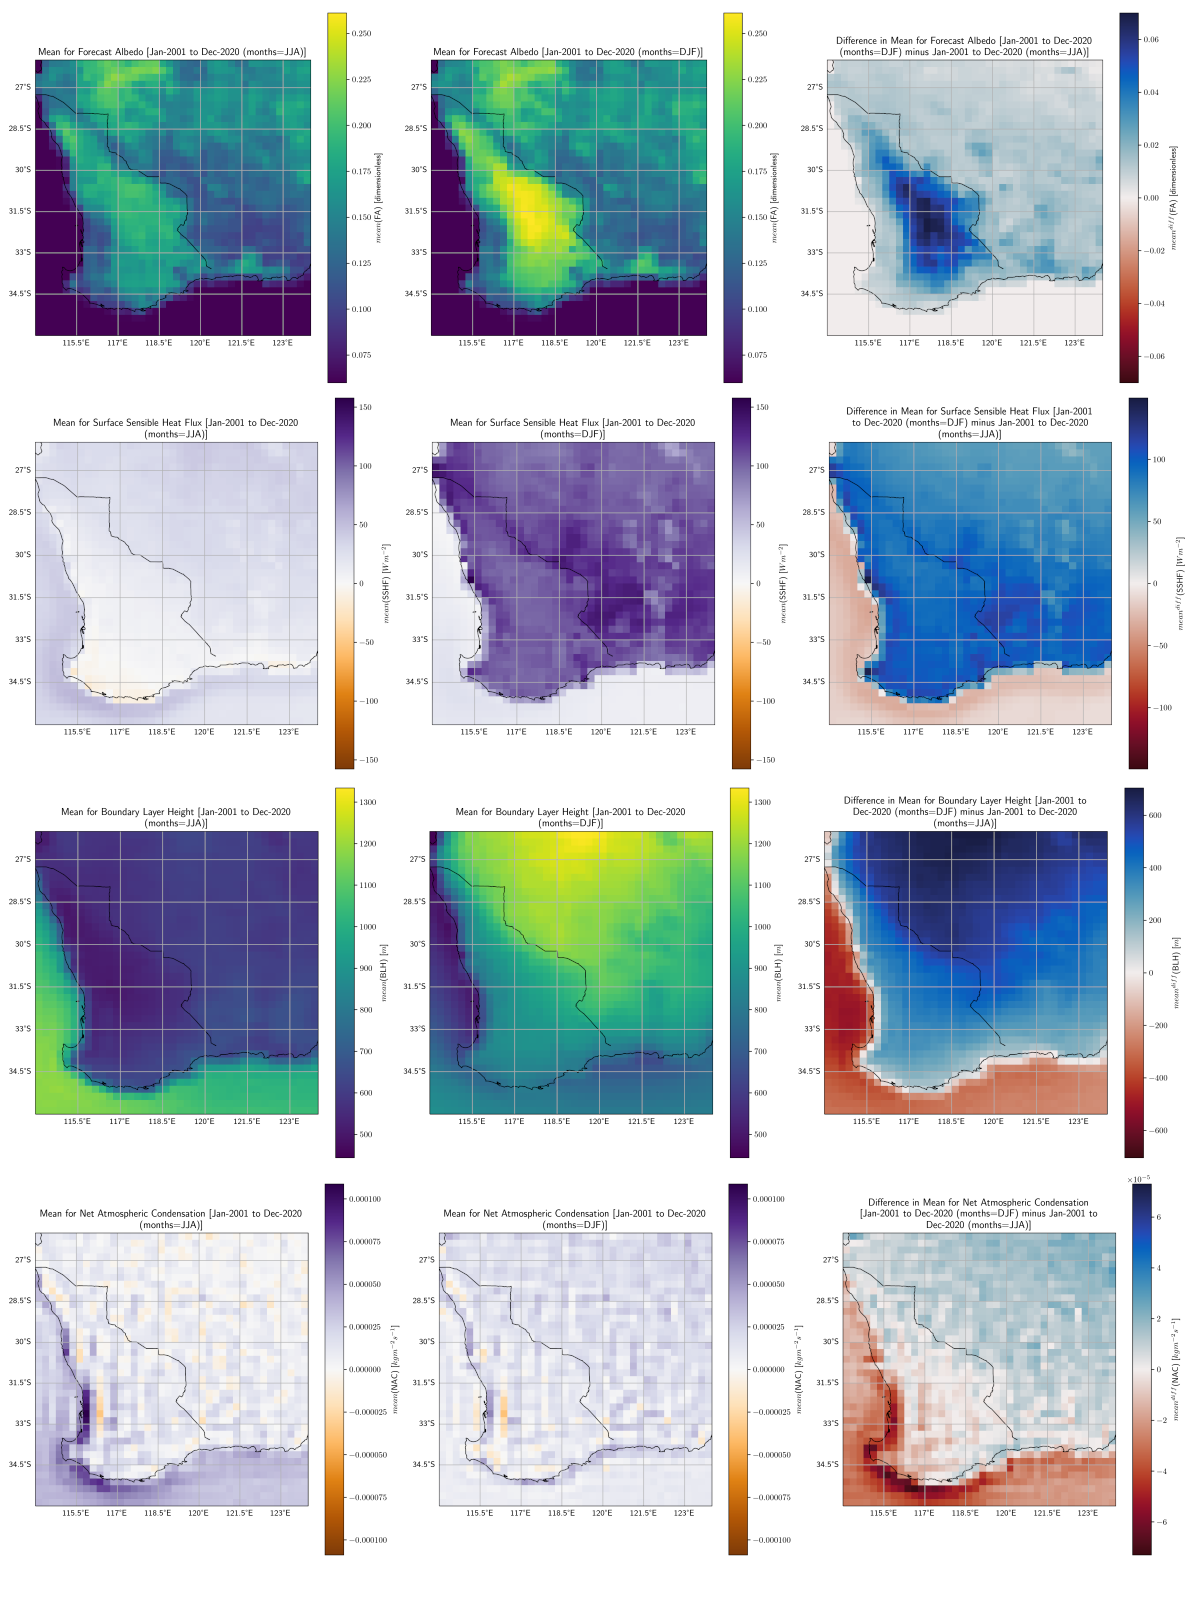
\includegraphics[width=0.9\textwidth]{wa_stats_seasonal_2.png}
	\caption[Selected MDP means with fence delineations]{\acs{MDP} means for \acs{FA}, \acs{SSHF}, \acs{BLH} and \acs{NAC} illustrate how the lower albedo of native vegetation leads to a thicker boundary layer via increased sensible heat for convective mixing, which in turn promotes increased atmospheric condensation (cloud formation).}
	\label{fig:wa_stats_seasonal_2}
\end{figure}

\subsubsection{Other contributions to NAC}

However, this may not be the full picture as the trends for \ac{SSHF}, \ac{BLH} and \ac{NAC} do not fully correlate with each other. \ac{BLH} appears to also be correlated with \ac{LSE} (compare with Figure~\ref{fig:wa_orog}) and this may possibly arise from wind shear effects.

\ac{CCN} particle size distributions resulting from native vegetation \ac{VOC} release forming \ac{SOA} may also affect \ac{NAC} patterns. Hourly means analysis reveals that night time condensation on the native side of the fence for \ac{DJF} is slightly higher than on the agricultural side of the fence, even when \ac{SSHF} is practically the same on both sides. If the \ac{CIAD} framework is valid, then another possible contribution is that moisture advection towards the native side of the fence (as observed in Figure~\ref{fig:wa_vidmf}) may then have a domino effect in making condensation further west of the fence more likely.

\subsubsection{Revisiting causation between VIEC and NAC}

Throughout the analysis of our results, we have turned to the question of whether positive \ac{NAC} (cloud formation) is primarily the result of negative \ac{VIEC} (rising air) or whether it is other way around (in line with the framework of \ac{CIAD}). Given that more positive \ac{NAC} in large part appears to directly result from surface energy balance effects, it calls into question yet again what additional causation \ac{VIEC} might have on top of this.

\paragraph{Contribution from SSHF}

There is very limited causation from \ac{VIEC} to \ac{SSHF} since the former is an atmospheric process and the latter is mostly a surface effect. So the remaining argument against \ac{CIAD} is either that \ac{SSHF} (perhaps in confluence with topography) produces the observed uplift of air masses which then leads to condensation (i.e.\ \ac{VIEC} is an intermediate cause between \ac{SSHF} and \ac{NAC}), or that \ac{SSHF} simultaneously causes similar patterns in \ac{VIEC} and \ac{NAC} via separate mechanisms (i.e.\ \ac{SSHF} is a confounding factor leading to a spurious correlation between \ac{VIEC} and \ac{NAC}).

\paragraph{SSHF alone cannot account for VIEC}

But neither of these seem to be the case because while the correlation between \ac{VIEC} and \ac{NAC} continues to hold during the \ac{JJA} months, hourly means analysis reveals that \ac{SSHF} actually displays the opposite trend to these variables as it does in \ac{DJF}. That is, \ac{SSHF} during \ac{JJA} is suppressed over agricultural land due to irrigation of crops, but all the while there is increased condensation with a very likely cause from increased evapotranspiration, and there is a correlated change to more \textit{negative} \ac{VIEC} values (more uplift) despite the \textit{decreased} \ac{SSHF}. Analogous results also apply on the native side of the fence with decreased evapotranspiration from native plants during \ac{JJA}. Furthermore, \ac{SSHF} is not at all correlated with any of the coastal effects observed in \ac{JJA} (see Section~\ref{ssec:coastal_cond}).

In summary, the idea that \ac{NAC} plays a causative role in \ac{VIEC} (possibly then leading to feedback) appears better supported by the available evidence than the idea that \ac{NAC} is a passive result of \ac{VIEC}.

\section{Similar comparison}

\subsection{Study periods}

\subsubsection{Selected periods}

For \ac{WA}, the selected periods for the similar comparison was from Jun-1997 to May-2002 and from Sep-2010 to Aug-2015 (see Figure~\ref{fig:wa_ind}). 

\begin{figure}[!ht]
	\centering
	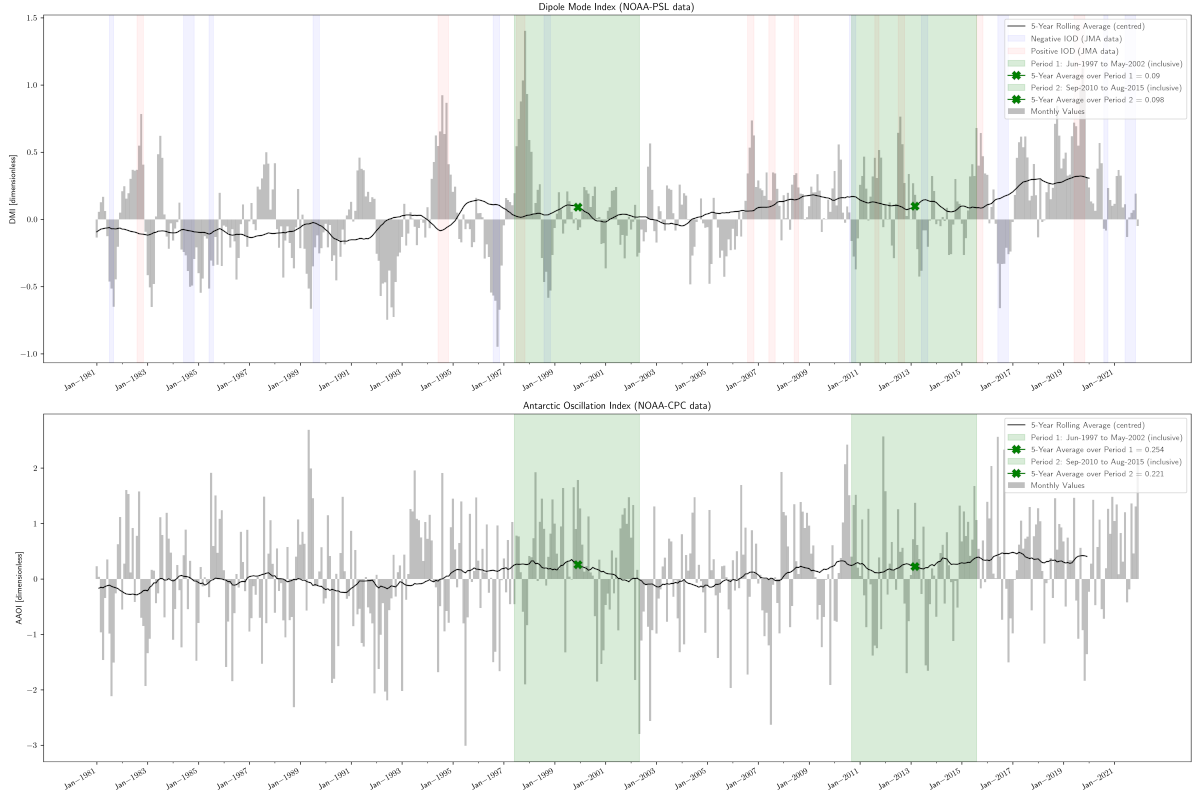
\includegraphics[width=0.9\textwidth]{wa_ind.png}
	\caption[WA's relevant climate indices for similar comparison]{\ac{NOAA} climate indices for climate drivers in \ac{WA}. Green shading highlights selected periods. Blue and red shading highlight negative and positive \ac{IOD} events respectively.}
	\label{fig:wa_ind}
\end{figure}

Between these periods was extensive vegetation loss concentrated along the coastal forests (see Figure~\ref{fig:wa_lai_similar}), resulting from a mix of drought events and human activities such as mining and forestry (beyond vegetation clearing, these activities are also implicated in causing a drop in the region's water table \citep{gordon2003, bauxite_hydro, johnson2003}).

\begin{figure}[!ht]
	\centering
	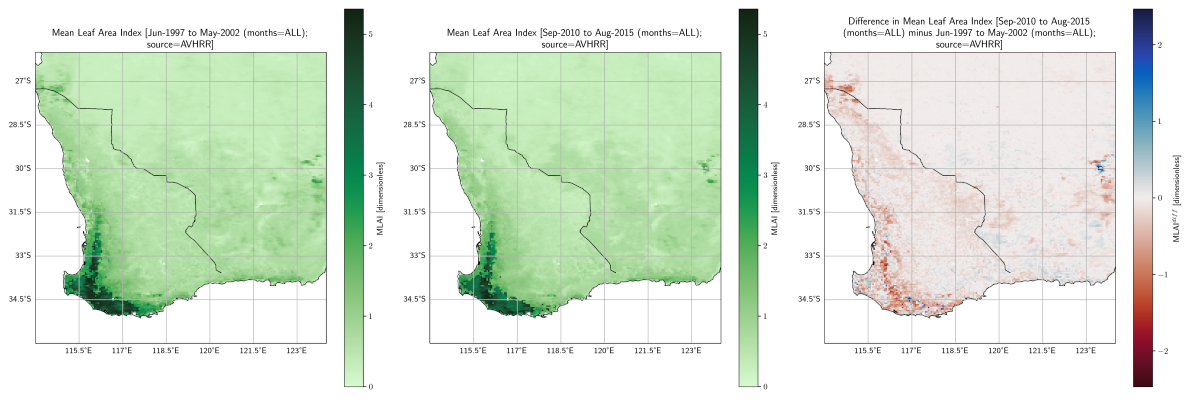
\includegraphics[width=0.9\textwidth]{wa_lai_similar.png}
	\caption[MLAI similar comparison for WA focus region]{\ac{MLAI} computed over each period in the similar comparison (left and middle), as well as the difference in these values between the two periods (right).}
	\label{fig:wa_lai_similar}
\end{figure}

\subsubsection{Comparable values in climate indices}

The main climate drivers for this region are the \ac{IOD} and \ac{AAO} (also known as \ac{SAM}) \citep{wa_drivers}. The corresponding indices are the \ac{DMI} and \ac{AAOI} respectively, and these = have similar averages over these periods. In fact, the 5-year averages over all the indices apart from the \ac{EPOI} (which is distant and not expected to have significant effects\footnote{Significant effects from teleconnections are possible but we have assumed this isn't the case here}.) have very similar values (not shown), although they appear to span across different phases for the longer-term oscillations.

\subsubsection{Summary of IOD events}

The period from Jun-1997 to May-2002 contains one Negative \ac{IOD} event and one Positive \ac{IOD} event, both of which display relatively high magnitudes for monthly values. Although the period from Sep-2010 to Aug-2015 contain two Negative \ac{IOD} events and two Positive \ac{IOD} events, each of these display relatively low magnitude in monthly values and so should still be comparable against the first period.

\subsection{Findings}
\label{ssec:similar_find}

No obviously remarkable correlations with coastal \ac{MLAI} loss was observed. Occasional delineations along forest cover did occur, but were too inconsistent to rule out the possibility of spurious relationships. It was also difficult to distinguish whether the occasional trends resulted from coastal \ac{MLAI} loss or modulation of atmospheric differences by the coast itself. However, sharp delineations along the fence are observed again in \ac{JJA} \ac{MDP} statistics despite minimal \ac{MLAI} loss around here, indicating that land cover imposes a local modulation upon changes in the synoptic background.

A change in \ac{JJA} synoptic conditions between periods sees an increase of \ac{MSLP} through the region despite increased \ac{T2}. The \ac{MSLP} increase in the northern part of the focus region is especially weak due to being offset by increased temperatures (especially on the native side of the fence). There is increased cloud formation (positive \ac{NAC}$^{diff}$) in subregions on the native side of the fence despite the increase in surface pressure. As with previous results, more positive \ac{NAC}$^{diff}$ correlates with more negative \ac{VIEC}$^{diff}$. \ac{VIEC}$^{diff}$, \ac{NAC}$^{diff}$ and \ac{VIDMF}$^{diff}$ all show sharp distinctions along the fence, with increased moisture convergence on the native side of the fence. See Figure~\ref{fig:wa_stats_similiar_1}.

While agricultural crops continued to transpire under the drier conditions, native vegetation reduced its transpiration, with a sharp decrease in its \ac{MDP} maximum. This in turn led to dramatic fence delineations in the \ac{MDP} maximum and minimum for \ac{NAC}, although this is partially confounded by \ac{ERA5} assimilation cycle artefacts (see Appendix~\ref{sec:artefact}). $range$(\ac{VIKE}) for \ac{JJA} continued to show delineation along the fence, but less so along the coastal forests, and a delineation is observed in the hour of \textit{minimum} rather than maximum. It is not clear what causes these \ac{VIKE} effects. See Figure~\ref{fig:wa_stats_similiar_2}.

%\enlargethispage{\baselineskip} % so you do not get a single line in another page
    \chapter{Discussion}

\section{Interpretation of results}

\section{Comparison with literature}

\section{Significance}

\section{Limitations and possible improvements}

\section{Future directions for research}

In an ideal world, you should have two kind of evaluations. The first is against some ground truth (perhaps a random model?). The second kind of evaluation is against other people's work (accuracy, speed, etc.). Any dimension which is of interest, should be evaluated.  Evaluation should be statistically sound.

\Blindtext

\section*{Summary}
\blindtext
    \chapter{Conclusions and Summary}
\label{ch:conclusions}

\begin{itemize}
	\item The results present strong evidence that the clearing of native vegetation for agriculture in southwest Western Australia has changed atmospheric energy conversions, in part due to changes in the surface energy balance.
	\item The results present strong evidence that land cover produces local modulations upon background synoptic changes, with typically dampened fluctuations.
	\item The results present moderate but indirect evidence (from water vapour flows) that surface wind circulation patterns will be affected beyond just effects from roughness length changes.
	\item The results present moderate evidence in support of the existence of condensation-induced atmospheric dynamics. This includes native vegetation modulation of atmospheric and moisture convergences leading to altered mass and moisture transport respectively.
	\item The results present moderate evidence that historical land cover change in southwest Western Australia has led to decreases in coastal temperatures which has weakened the summer daytime sea breeze. This has likely caused the observed inland rainfall loss, decreased inland moisture convergence (possibly indicting wind convergence), and an increased coastal flood risk. Meanwhile, the effect of future land cover change is highly variable depending on what type of change takes place.
	\item For wind energy operation, the implications for this are decreased generation and operating revenue during peak season, increased risk of infrastructure damage from floods, and increased risk embodied from uncertainty regarding what future land cover change will take place. A weakened sea breeze also implies less cool relief to the urban centre of Perth during summer daytime, so a decrease in supply coincides with an increase in demand (see Section~\ref{ssec:implications}).
	\item A conceptual framework for understanding how land cover affects surface winds was created, along with a heuristical procedure for qualitatively assessing the likely effect of future land cover change on circulation patterns.
	\item A series of purpose-built Python programs was developed for analysing how vegetation change affects the diurnal and seasonal variations of an arbitrary variable from the \ac{ERA5} dataset (see Appendix~\ref{app:code}).
\end{itemize}

%\enlargethispage{\baselineskip} % so you do not get a single line in another page
    \appendix
        \chapter{Supplementary information}
\label{app:supp}

\section{Unmarked figures}
\label{sec:unmarked}

\subsection{January means for selected variables 1 (unmarked)}

The use of coloured markings with thick outline in Figure~\ref{fig:wa_jan_comb_1} somewhat distorts perception of the trends. For an undistorted view, see the January mean values for \ac{VIEC}, \ac{NAC}, \ac{VIDMF} and \ac{NSE} in Figure~\ref{fig:wa_jan_comb_1_unmarked}.

\begin{figure}[!htp]
	\centering
	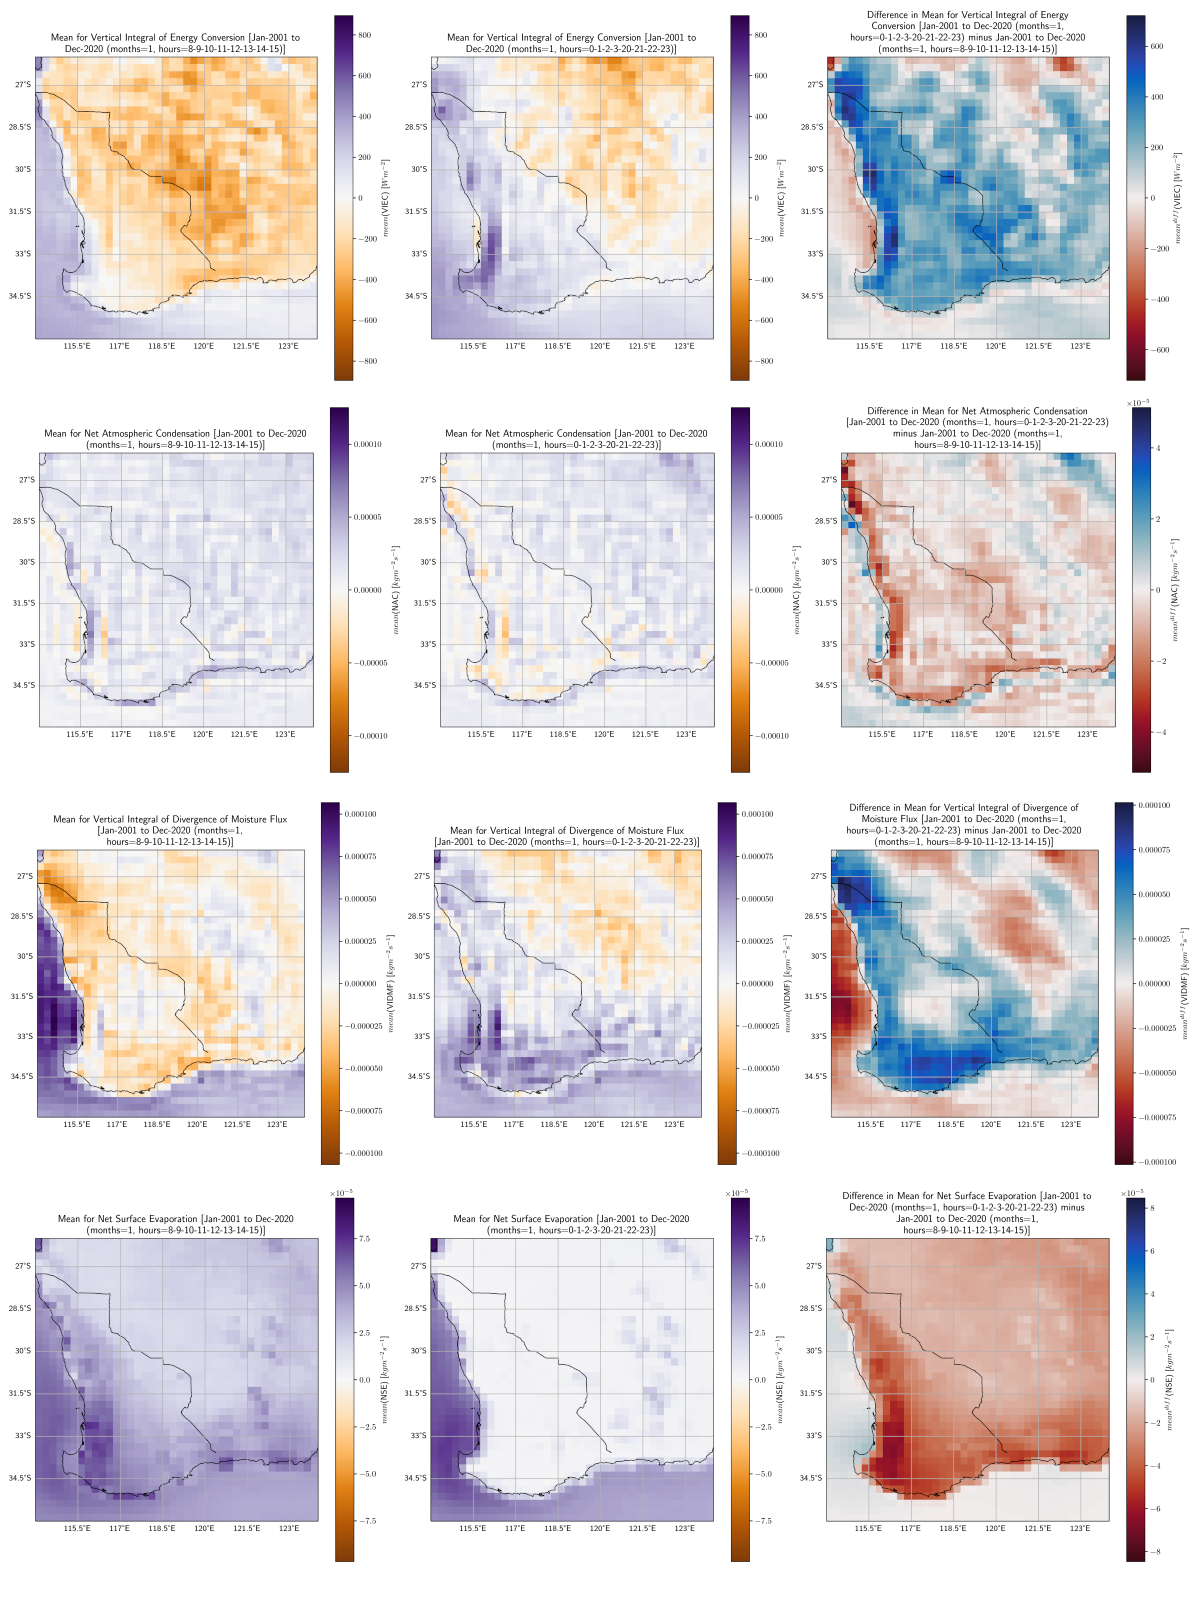
\includegraphics[width=0.9\textwidth]{wa_jan_comb_1_unmarked.png}
	\caption[January means for selected variables 1 (unmarked)]{January mean daytime and nighttime values for \acs{VIEC}, \acs{NAC}, \acs{VIDMF} and \acs{NSE}.}
	\label{fig:wa_jan_comb_1_unmarked}
\end{figure}

\subsection{January means for selected variables 2 (unmarked)}

The use of coloured markings with thick outline in Figure~\ref{fig:wa_jan_comb_2} somewhat distorts perception of the trends. For an undistorted view, see the January mean values for \ac{WS100}, \ac{dWS100}, \ac{MSLP} and \ac{T2} in Figure~\ref{fig:wa_jan_comb_2_unmarked}.

\begin{figure}[!htp]
	\centering
	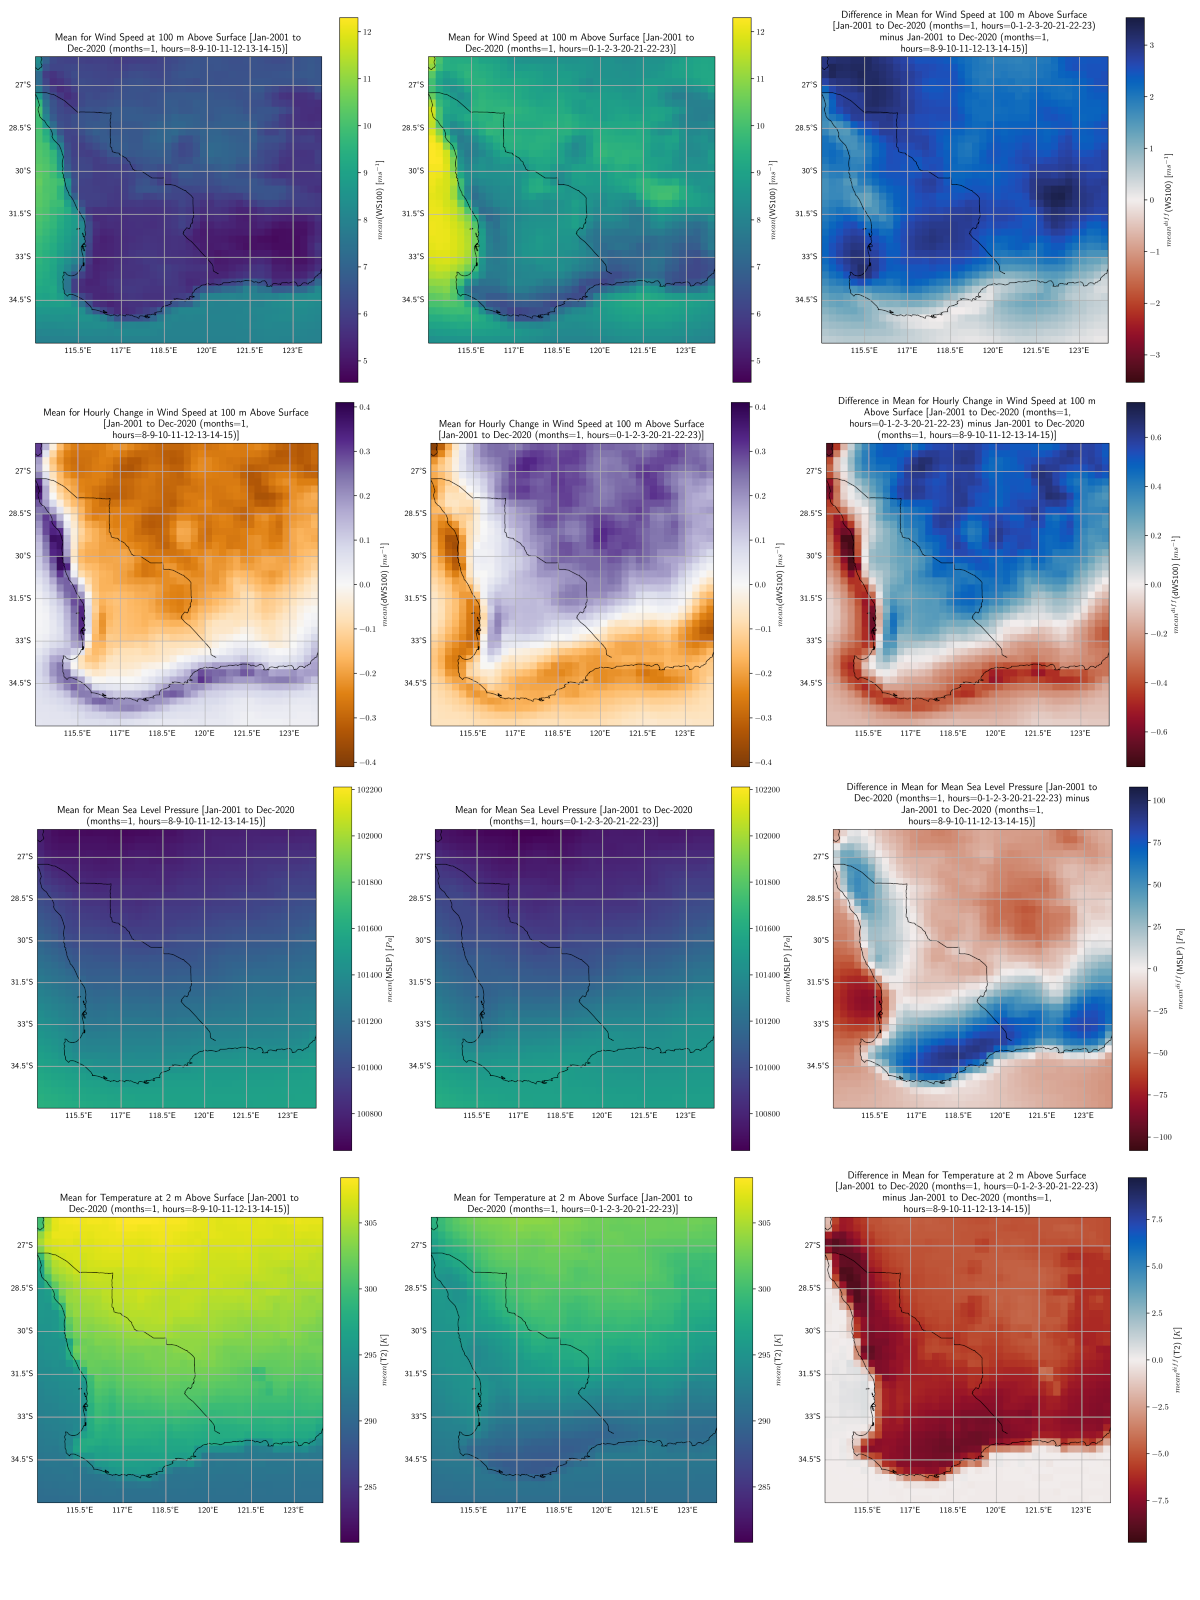
\includegraphics[width=0.9\textwidth]{wa_jan_comb_2_unmarked.png}
	\caption[January means for selected variables 2 (unmarked)]{January mean daytime and nighttime values for \acs{WS100}, \acs{dWS100}, \acs{MSLP} and \acs{T2}.}
	\label{fig:wa_jan_comb_2_unmarked}
\end{figure}

\section{Full list of study variables}

Some of the key variables studied in this project were presented in Section~\ref{sec:method_var}. For a full list of variables used in this study, including those which were analysed but for which there were no significant findings, see Table~\ref{tab:vars_analysis}.

\newcolumntype{P}[1]{>{\centering\arraybackslash}p{#1}}
\begin{landscape}
	%	\pagestyle{empty} %% only if you want to remove silly headers on the side	
	\begingroup
	\renewcommand\arraystretch{1.33} % only applicable to this table because of group
	
	\begin{longtable}{P{2cm}P{3cm}P{13cm}}
		\caption[Full list of study variables]{A full list of variables which were analysed. Abbreviations for these variables as used in the report are provided, along with descriptions of each variable.} 
		\label{tab:vars_analysis} 
		\\ 
		\toprule 
		\multicolumn{1}{P{2cm}}{\textbf{Abbreviation}}
		& \multicolumn{1}{P{3cm}}{\textbf{Variable}}
		& \multicolumn{1}{P{15cm}}{\textbf{Description}}\\	
		\midrule
		\endfirsthead
		\midrule
		\multicolumn{1}{P{2cm}}{\textbf{Abbreviation}}
		& \multicolumn{1}{P{3cm}}{\textbf{Variable}}
		& \multicolumn{1}{P{15cm}}{\textbf{Description}}\\	
		\midrule	
		\endhead
		\midrule	
		\multicolumn{3}{l@{}}{(continued\ldots)}\\
		\endfoot
		\endlastfoot
		\acs{LSE} & Land Surface Elevation & Units in $m$. Elevation of the land surface above sea level. Obtained by converting from ERA5 geopotential data using the MetPy Python library \citep{metpy}. \\
		\acs{SSGO} & Slope of Sub-Gridscale Orography & Dimensionless. Represents slopes of orographic features such as mountains and hills which are present down to a scale of 1 km. Flat surfaces have value 0 while vertical cliffs have value 1. \\ \midrule
		\acs{MLAI} & Mean Leaf Area Index & Dimensionless. The \ac{LAI} index for a grid cell is the total leaf area divided by ground area of that cell. \ac{MLAI} is the mean of this over the study period. This was the main metric used in assessing vegetation cover and vegetation cover change.  \\
		\acs{MFAPAR} & Mean Fraction of Photosynthetically Absorbed Radiation & Dimensionless. The \ac{FAPAR} for a grid cell is the fraction of radiation between 400-700 nm wavelength absorbed within that cell. \ac{MFAPAR} is the mean of this over the study period. This was a supplementary metric used in assessing vegetation cover and vegetation cover change. \\ \midrule
		\acs{BLH} & Boundary Layer Height & Units in $m$. Height of the depth of air for which surface effects are significant. This was used to assess level of convective mixing and likelihood fo cloud formation. \\
		CAPE & Convective Available Potential Energy & Units in $J kg^{-1}$. Work which would be performed on an air parcel if it rose through the atmosphere. This was used to indicate atmospheric stability. The more positive the more air will rise, the more negative the more air will sink. \\
		\acs{CBH} & Cloud Base Height & Units in $m$. Height for base of lowest cloud. This was used to assess how height of cloud formation may affect atmospheric circulations. \\
		FA & Forecast Albedo & Dimensionless. Fraction of short-wave radiation reflected from surface. This was used to assess how reflectivity of different land cover affects the surface energy balance. \\
		\acs{MSLP} & Mean Sea Level Pressure & Units in $Pa$. Pressure of atmosphere adjusted to sea level. This is one of the main variables affecting wind. High values typically coincide with calm conditions while low values coincide with windy. This was also used to identify synoptic features. \\
		\acs{NAC} & Net Atmospheric Condensation & Units in $kg m^{-2} s^{-1}$. Condensation minus evaporation in atmosphere (does not include surface). Positive values indicate more cloud formation than cloud evaporation. Calculated using \ac{ERA5} data for \ac{TCWV}, \ac{NSE} and \ac{VIDMF} (see Appendix~\ref{sec:nac_derive}). This is one of the major factors affecting the partitioning of the atmospheric energy budget. \\
		\acs{NSE} & Net Surface Evaporation & Units in $kg m^{-2} s^{-1}$. Evaporation minus condensation at surface (does not include atmosphere). For vegetation, positive values indicate a greater amount of evapotranspiration than dew formation. Instantaneous values are approximated by averaging consecutive \ac{ERA5} accumulation values.\footnote{\ac{ERA5} parameters come in instantaneous and accumulation values. Instantaneous values are calculated for that point in time at each hour whereas accumulation values represent a sum compiled over the course of the previous hour window. \ac{NSE}, \ac{SLHF} and \ac{SSHF} are accumulation values whereas the remainder are instantaneous. Averages for these variables were computed to approximate "instantaneous" values in order to allow an apples to apples comparison.} \\
		\acs{SLHF} & Surface Latent Heat Flux & Units in $W m^{-2}$. Rate at which energy at the surface is being used for evapotranspiration. Instantaneous values are approximated by averaging consecutive \ac{ERA5} accumulation values (see \ac{NSE} footnote). \\
		\acs{SSHF} & Surface Sensible Heat Flux & Units in $W m^{-2}$. Rate at which energy at the surface is being used to induce convection and warming of the air mass above it. Instantaneous values are approximated by averaging consecutive \ac{ERA5} accumulation values (see \ac{NSE} footnote). \\
		\acs{T2} & Temperature at 2 m Above Surface & Units in $K$. This is one of the major factors affecting the partitioning of the atmospheric energy budget. \\
		\acs{TCC} & Total Cloud Cover & Dimensionless. Fraction of grid cell covered by cloud. \\
		\acs{TCCLW} & Total Column Cloud Liquid Water & Units in $kg m^{-2}$. Total cloud liquid content averaged over grid cell. Does not include rain water droplets. \\
		\acs{TCWV} & Total Column Water Vapour & Units in $kg m^{-2}$. Total amount of water vapour averaged over grid cell. Often referred to as precipitable water (PW). \\
		\acs{U10} & Zonal Component of 10 m Wind Velocity & Units in $m s^{-1}$. East-West component of wind velocity at 10 m above surface. Positive values indicate that wind has a westerly component (blowing \textit{to} the east). \\
		\acs{U100} & Zonal Component of 10 m Wind Velocity & Units in $m s^{-1}$. East-West component of wind velocity at 100 m above surface. Positive values indicate that wind has a westerly component (blowing \textit{to} the east). \\
		\acs{V10} & Meridional Component of 10 m Wind Velocity & Units in $m s^{-1}$. North-South component of wind velocity at 10 m above surface. Positive values indicate that wind has a southerly component (blowing \textit{to} the north). \\
		\acs{V100} & Meridional Component of 100 m Wind Velocity & Units in $m s^{-1}$. North-South component of wind velocity at 100 m above surface. Positive values indicate that wind has a southerly component (blowing \textit{to} the north). \\
		\acs{VIDMF} & Vertical Integral of Divergence of Moisture Flux & Units in $kg m^{-2} s^{-1}$. The average rate at which water vapour in a grid cell is leaving to neighbouring grid cells.\footnote{Note that \ac{ERA5} has a similarly named parameter called \ac{VIMF} which is an accumulation rather than instantaneous parameter, but with the crucial difference that "moisture" in this variable refers to the total of water vapour, cloud liquid and cloud ice. The ERA5 documentation for \ac{VIDMF} also refers to "moisture" and it is not apparent that this actually uses a different definition where it only includes water vapour, but this was indeed confirmed to be the case via correspondence with \ac{ECMWF} specialist support.} Positive values indicate water vapour is diverging (leaving grid cell) while negative values indicate water vapour is converging (entering grid cell). \\
		\acs{VIEC} & Vertical Integral of Energy Conversion & Units in $W m^{-2}$. Rate at which energy is being converted from internal plus potential energy into kinetic energy.\footnote{By \ac{ERA5} definitions, internal energy refers to the microscopic energy of the air molecules excluding latent energy (this is treated as a separate part of the atmospheric energy budget) which may be different to definitions used in chemistry. Potential energy here refers to macroscopic gravitational potential energy (as opposed to internal air pressure within the grid cell, as this is implicitly accounted for within internal energy). Kinetic energy refers to kinetic energy from the \textit{horizontal} motion of air masses.} Negative values indicate kinetic energy conversion into internal plus potential energy. \\
		\acs{VIKE} & Vertical Integral of Kinetic Energy & Units in $J m^{-2}$. Total kinetic energy from the \textit{horizontal} motion of air masses through the grid cell, averaged over the grid cell. This was used to study how land cover change affects partitioning in the atmospheric energy budget. \\
		\acs{VIPILE} & Vertical Integral of Potential, Internal and Latent Energy & Units in $J m^{-2}$. Total of gravitational potential energy, internal energy and latent energy (see footnote for \ac{VIEC}). This constitutes the total atmospheric energy budget minus kinetic energy. This was used to study how land cover change affects partitioning in the atmospheric energy budget. \\
		\acs{WS10} & Wind Speed at 10 m Above Surface & Units in $m s^{-1}$. Scalar quantity for wind speed at 10 m above surface. \\
		\acs{WS100} & Wind Speed at 100 m Above Surface & Units in $m s^{-1}$. Scalar quantity for wind speed at 100 m above surface. This is the quantity most directly relevant for wind energy generation. \\
		\acs{WV10} & Wind Velocity at 10 m Above Surface & Units in $m s^{-1}$. Vector quantity for wind velocity at 10 m above surface. \\
		\acs{WV100} & Wind Velocity at 100 m Above Surface & Units in $m s^{-1}$. Vector quantity for wind velocity at 100 m above surface. This quantity is also directly relevant for wind energy generation and furthermore highlights how wind direction changes. \\ \midrule
		d\{VAR\} & Hourly Change in \{VAR\} & Units vary. Change in the value for each of the above \ac{ERA5} or \ac{ERA5}-derived values, as compared with its value in the previous hour. This was used to study how the rate of change of a variable was correlated with land cover change. \\ \midrule
		\acs{C10} & Weibull Scale Parameter for 10 m Wind Speed & Units in $m s^{-1}$. Scale parameter for the Weibull distribution fit to the wind speed at 10 m above surface. The empirical Weibull fit was obtained using the equations of \citep{justus1977}. \\
		\acs{C100} & Weibull Scale Parameter for 100 m Wind Speed & Units in $m s^{-1}$. Scale parameter for the Weibull distribution fit to the wind speed at 100 m above surface. The empirical Weibull fit was obtained using the equations of \citep{justus1977}. \\
		\acs{EROE100} & Expected Rate of 100 m Wind Speed Exceeding 42.5 m/s & Dimensionless. The \textit{expected} rate for wind speed at 100 m exceeding 42.5 m/s, which in practice is the typical wind speed which wind turbines can last 10 mins in before failure \citep{chen2015, chen2016, ge_web}. This is the \textit{expected} rate calculated from the tail of the Weibull distribution fit rather than the actual observed rate of exceedance. \\
		\acs{K10} & Weibull Shape Parameter for 10 m Wind Speed & Dimensionless. Shape parameter for the Weibull distribution fit to the wind speed at 10 m above surface. The empirical Weibull fit was obtained using the equations of \citep{justus1977}. \\
		\acs{K100} & Weibull Shape Parameter for 100 m Wind Speed & Dimensionless. Shape parameter for the Weibull distribution fit to the wind speed at 100 m above surface. The empirical Weibull fit was obtained using the equations of \citep{justus1977}. \\
		$mean$(\acs{WS10}) & Mean of 10 m Wind Speed & Units in $m s^{-1}$. Mean of wind speed at 10 m above surface. This is roughly equivalent to the mean of the mean diurnal profile for \ac{WS10} (see Section~\ref{ssec:mean_commute}). \\
		$mean$(\acs{WS100}) & Mean of 100 m Wind Speed & Units in $m s^{-1}$. Mean of wind speed at 10 m above surface. This is roughly equivalent to the mean of the mean diurnal profile for \ac{WS100} (see Section~\ref{ssec:mean_commute}). \\
		$std$(\acs{WS10}) & Standard Deviation of 10 m Wind Speed & Units in $m s^{-1}$. Standard deviation of wind speed at 10 m above surface. This is used with \ac{K10} to analyse how the variability in wind speed changes along with land cover. \\
		$std$(\acs{WS100}) & Standard Deviation of 100 m Wind Speed & Units in $m s^{-1}$. Standard deviation of wind speed at 10 m above surface. This is used with \ac{K100} to analyse how the variability in wind speed changes along with land cover. \\
		\acs{TGCF100} & Typical Gross Capacity Factor for 100 m Turbine & Dimensionless. Gross capacity factor which a typical 2.5 MW turbine with 100 m hub height would have had over the study period. This was computed by first averaging the power curves for similar 2.5 MW turbines from Vestas, Goldwind and GE Energy, then computing the energy generation for each hour in the study period using \ac{ERA5} data for the wind speed at 100 m above surface (see Section~\ref{ssec:method_wsd}). \\ \bottomrule
	\end{longtable}
	
	\endgroup
\end{landscape}

\section{Assimilation cycle artefacts in ERA5}
\label{sec:artefact}

\subsection{Artefacts in TCWV}

The hourly mean results for \ac{dTCWV} at hours 0600 \ac{LT} (2200 UTC) and 1800 \ac{LT} (1000 UTC) indicate a discontinuous change in \ac{TCWV} (not shown). These values represent the change in \ac{TCWV} from 2100-2200 UTC and 0900-1000 UTC respectively. The humidity (and by extension \ac{TCWV}) values in ERA5 are known to have a mismatch between the end of one assimilation cycle and the beginning of the next, which happen at exactly these time windows \citep{ecmwf}.

\subsection{Artefacts inherited by NAC}

Because the \ac{NAC} value at hour i is derived using the \ac{TCWV} values at hours i-1 and i+1 (see Appendix~\ref{sec:nac_derive}), the \ac{NAC} value at hours 0500-0700 \ac{LT} and 1700-1900 \ac{LT} inherit these discontinuities (see Figure~\ref{fig:wa_dnac_artefact}). These discontinuities are not observed for any of the other variables which \ac{NAC} is derived from (\ac{NSE} and \ac{VIDMF}).

\begin{figure}[!htp]
	\centering
	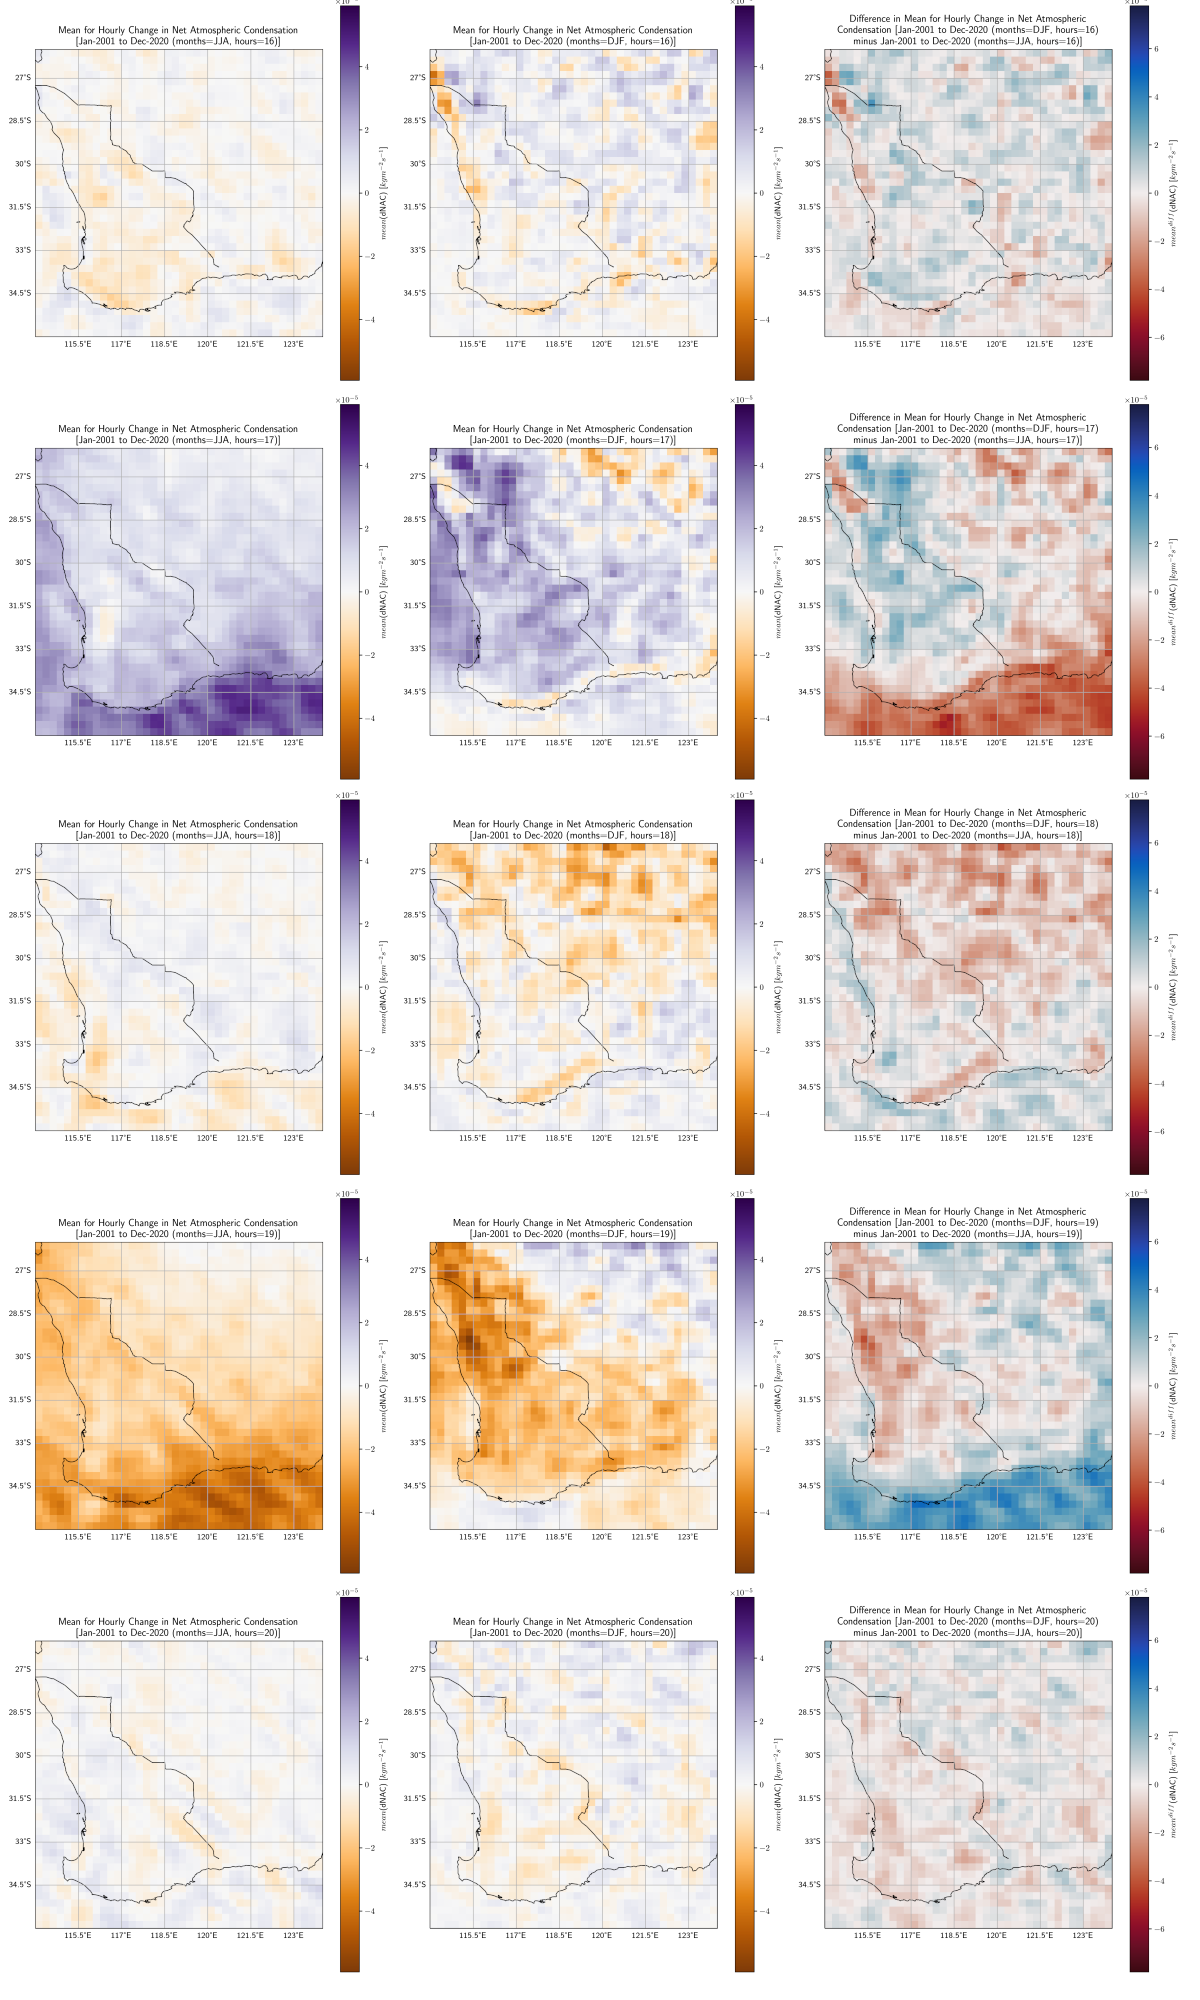
\includegraphics[width=0.75\textwidth]{wa_dnac_artefact.png}
	\caption[1600-2000 means for dNAC (artefacts)]{1600-2000 mean \ac{JJA} and \ac{DJF} values for \acs{dNAC}. 1600 and 2000 means are in line with means in remaining hours. Artefacts inherited from \ac{TCWV} assimilation cycles show opposite trends at 1700 and 1900.}
	\label{fig:wa_dnac_artefact}
\end{figure}

\subsection{Results relatively unaffected}

Figure~\ref{fig:wa_dnac_artefact} shows how this leads to unusually large \ac{dNAC} means from 1700-1900 \ac{LT}. But importantly, the increases at 1700 \ac{LT} are offset by a spatially correlated decrease of comparable magnitude at 1900 \ac{LT}. Analogous results were found between 0500-0700 \ac{LT} (not shown). So the means computed over the course of this project should be relatively unaffected. This applies even for the diurnal comparison where means were computed over a subset of hours, since daytime and nighttime hours were defined as 0800-1500 \ac{LT} and 2000-0300 \ac{LT} respectively (see Section~\ref{ssec:method_diurnal_seasonal}), which falls outside of the hours with artefacts. This does mean, however, that \ac{MDP} statistics apart from the mean (hour of maximum, hour of minimum, maximum, minimum and range) need to be interpreted with care when it comes to \ac{TCWV}, \ac{dTCWV}, \ac{NAC} and \ac{dNAC}. 

\subsection{Other affected variables}

None of the other key study variables apart from \ac{FA} were found to have similarly obvious assimilation cycle discontinuities, but \ac{FA} was only used for one result (Figure~\ref{fig:wa_stats_seasonal_2}) which was a mean over all hours of the day so results should still be relatively unaffected.

\section{Other focus regions in original project scope}
\label{sec:other_regions}

The original project scope included results for \ac{CA} and \ac{NB} but time did not allow for detailed analysis, discussion and presentation of these results. Included below is a summary for each of these regions, as well as the selected periods for the similar comparison. This may be used for future research.

\subsection{General}

\subsubsection{Periods for diurnal and seasonal comparison}

For all focus regions, the diurnal and seasonal comparisons were performed over the period from Jan-2001 to Dec-2020 (inclusive). The GLASS products derived from \ac{MODIS}, the more advanced instrument, begin around Mar-2000, with the \ac{LAI} dataset ending Dec-2021 while the \ac{FAPAR} dataset ends Dec-2020 (at the time of writing). As averages starting from Mar-2000 and ending Dec-2020 would have skewed weightings for the months of January and February, we elected to use Jan-2001 as the period start instead.

\subsubsection{Wet and dry months}

Based on historical precipitation climatology, we have selected the months representing the wet and dry seasons for each region as being:
\begin{itemize}
	\item \ac{WA}: June, July, August (JJA) and December, January, February (DJF) respectively
	\item \ac{CA}: May to October (5-6-7-8-9-10) and November to April (1-2-3-4-11-12) respectively
	\item \ac{NB}: January to June (1-2-3-4-5-6) and July to December (7-8-9-10-11-12)
\end{itemize}

\subsubsection{Daytime and nighttime hours}

The local timezones for \ac{WA}, \ac{CA} and \ac{NB} are UTC+8, UTC-6 and UTC-3 respectively\footnote{The focus region for \ac{NB} spans across 35 degrees of longitude, so it actually covers multiple local timezones and over more than 2 hours of local solar timezones (15 degrees per hour). We have selected UTC-3 here because this is close to the local solar timezone for the midpoint of this region.}. Where comparisons between daytime and nighttime hours have been made, the average values for hours from 8 am to 3 pm local time\footnote{Unless otherwise stated, all times in this report are expressed in local time, and hour endpoints are inclusive.} (8-9-10-11-12-13-14-15) have been selected as representative of daytime, while the average values for hours from 8 pm to 3 am local time (0-1-2-3-20-21-22-23) have been selected as representative of nighttime.

\subsubsection{Orography}

The orography for each focus region is displayed in Figure~\ref{fig:orog}.

\begin{figure}[!ht]
	\centering
	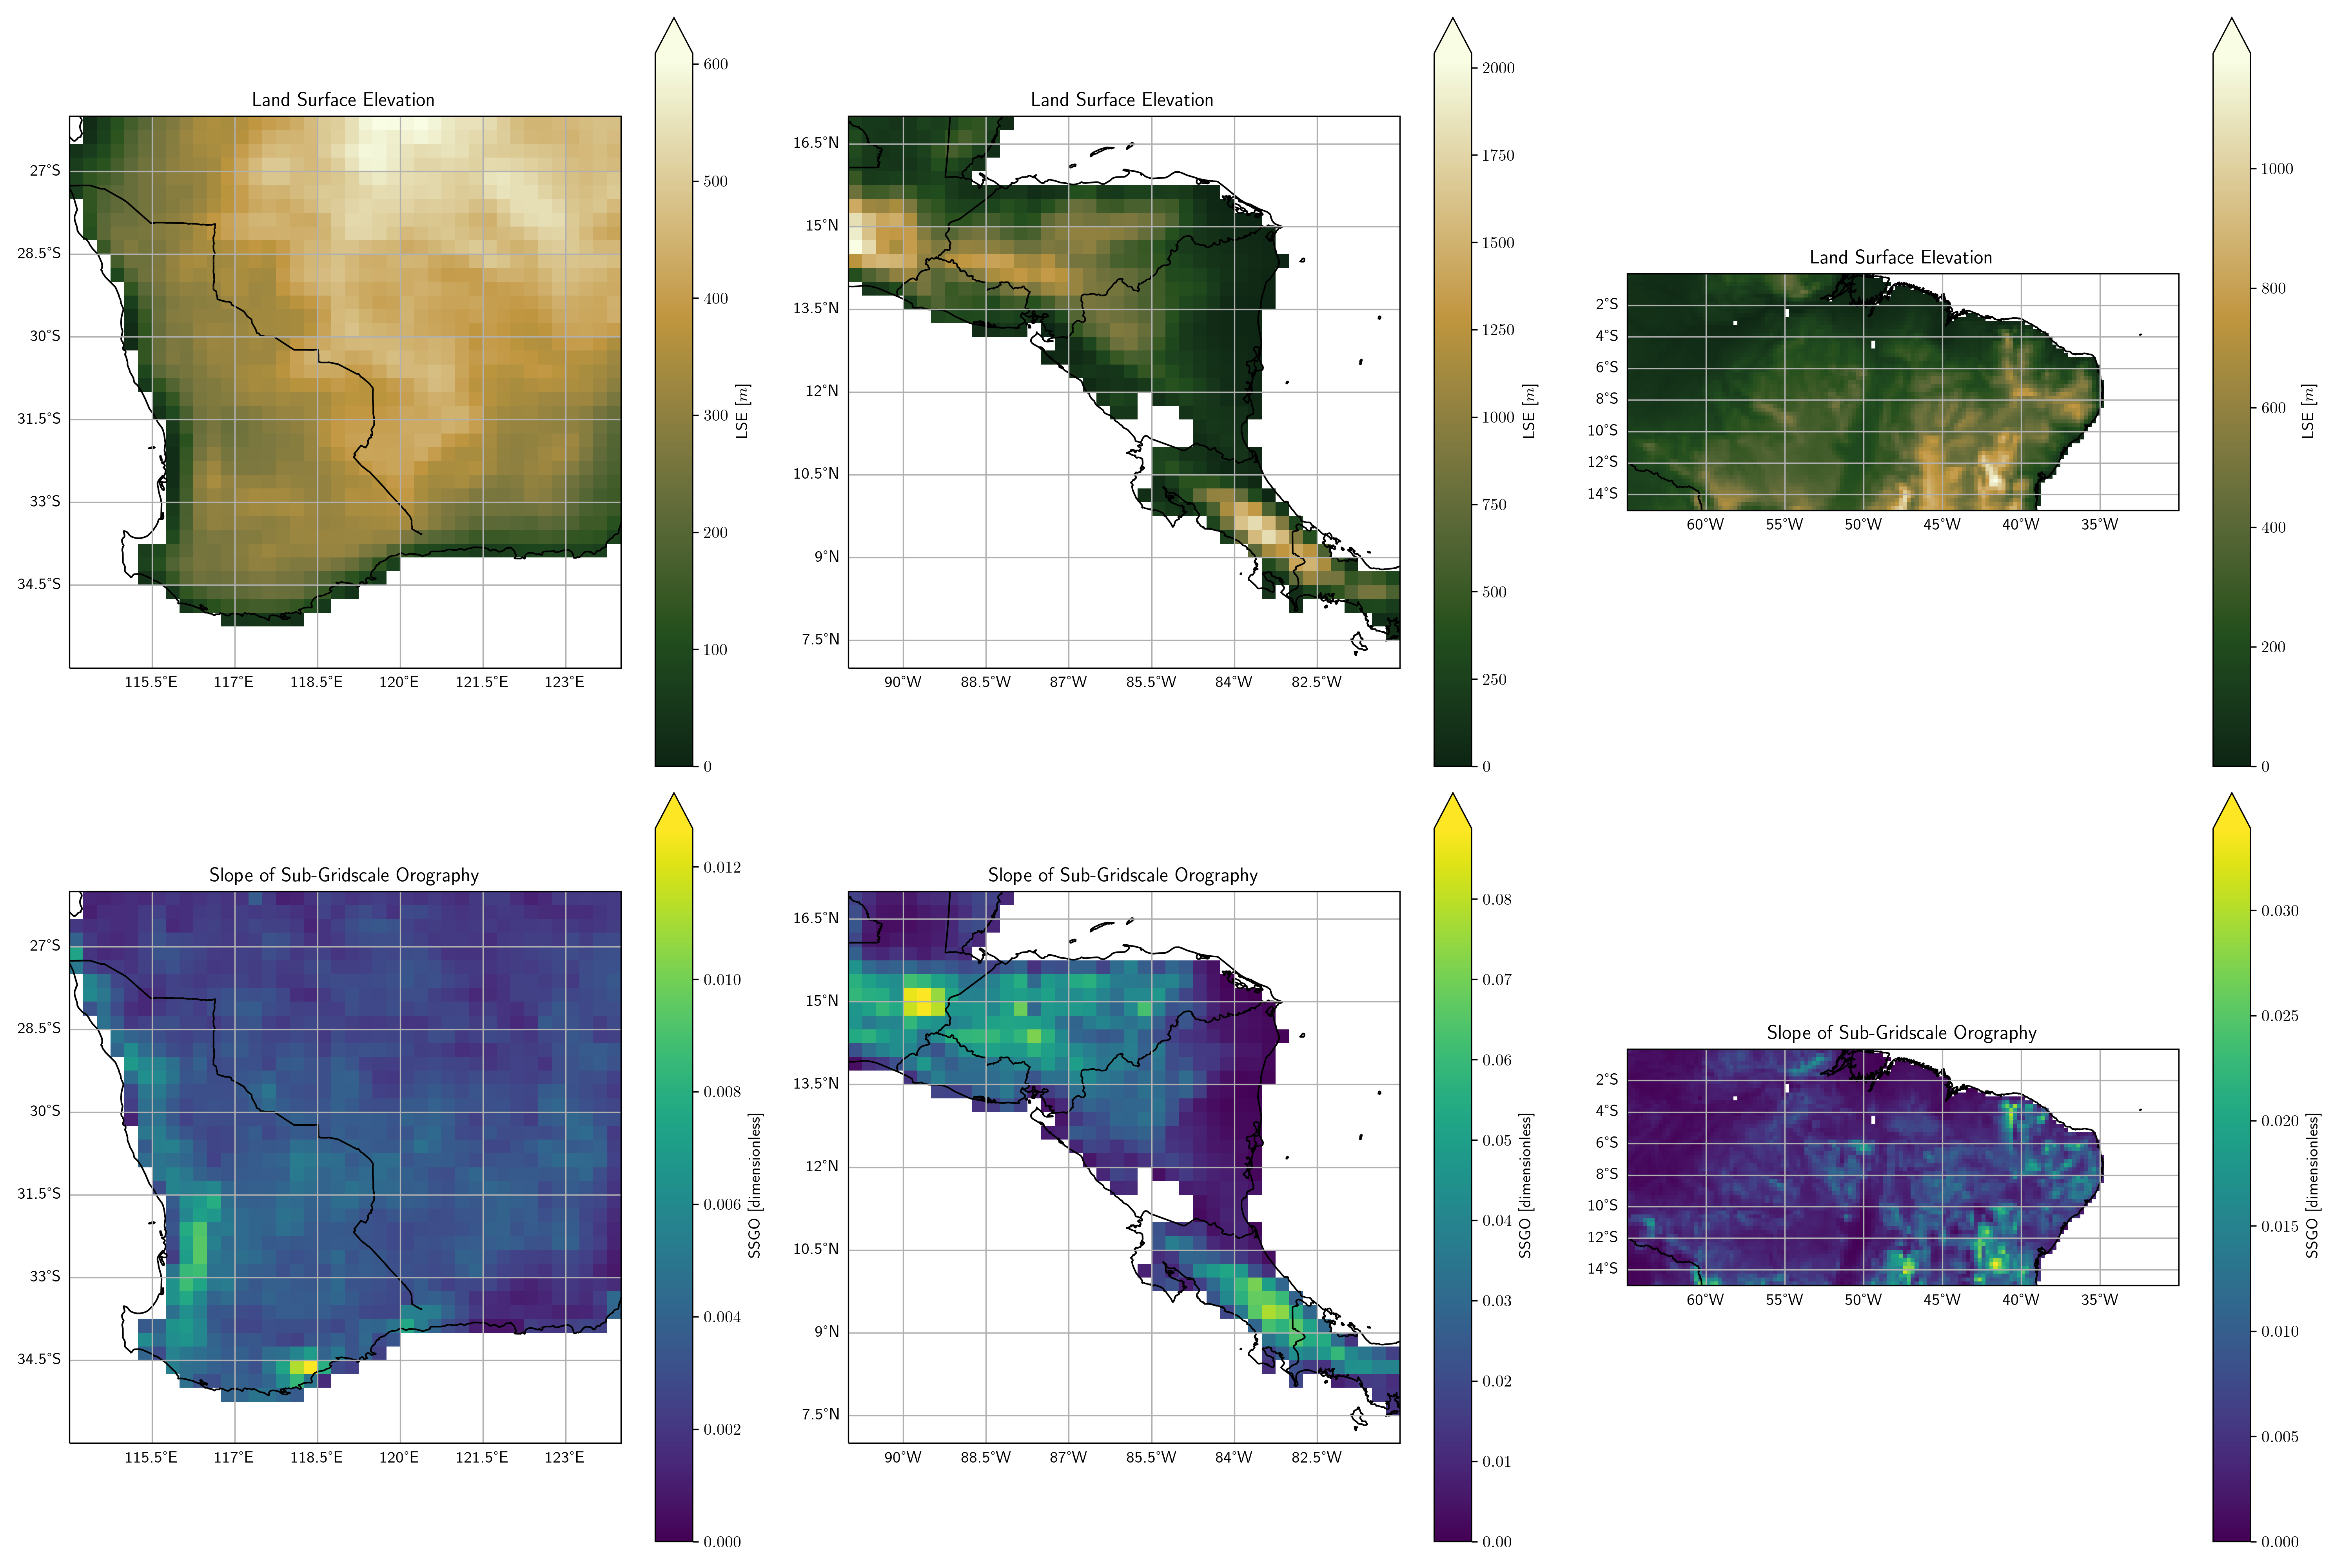
\includegraphics[width=0.9\textwidth]{orog.png}
	\caption[Orography for all focus regions]{Top row: \acf{LSE} for each region. Bottom row: \acf{SSGO} for each region. From left to right: \acl{WA}, \acl{CA}, \acl{NB}.}
	\label{fig:orog}
\end{figure}

\subsection{Central America}

\begin{figure}[!ht]
	\centering
	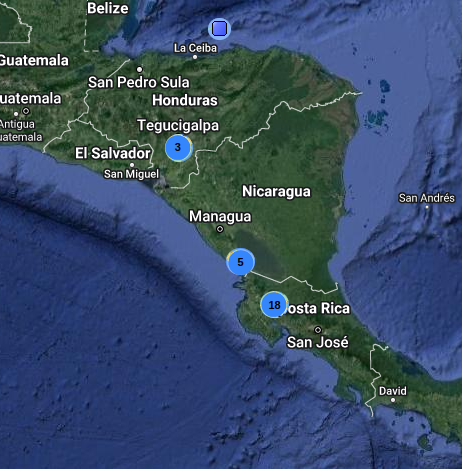
\includegraphics[width=0.75\textwidth]{maps_twp_ca}
	\caption[Central America Map]{Satellite image displaying Central America focus region from 91$^\circ$W to 81$^\circ$W longitude and 17$^\circ$S to 7$^\circ$S latitude \citep{maps_ca}. Markers indicating positions and number of wind farms have been edited on using data from \citep{twp_hd, twp_nc, twp_cr}.}
	\label{fig:maps_twp_ca}
\end{figure}

\subsubsection{Description of region}

We selected the part of \ac{CA} which runs (North to South) from El Salvador and Honduras to Nicaragua to Costa Rica (91$^\circ$W to 81$^\circ$W longitude and 17$^\circ$S to 7$^\circ$S latitude; see Figure~\ref{fig:maps_twp_ca}) because there existed spatially opposing trends in vegetation change. These countries had historically comparable rates of deforestation, but Costa Rica shifted towards reforestation due to policy changes in the 1990s whereas deforestation has continued in Honduras and Nicaragua. The western coastlines for El Salvador, Nicaragua and Costa Rica (where agriculture is concentrated) also have comparable cardinal orientations.

Being located near the equator, annual temperature variation at these locations are relatively minor. This is useful because it provides a comparison where one of the main variables affecting wind flow is relatively controlled for. Furthermore, the entire focus region is on the order of 1000 km, so synoptic weather features (which have a characteristic scale of this order) are less likely to produce contrasting effects over the different subregions.

\subsubsection{Significance of results from this region}

Wind farms are concentrated on agricultural land along the western coast where there are plans for continued development. But as in the case of \ac{WA}, the value of this focus region isn't necessarily in its direct implications for existing wind farms in the area, but in that it may yield some insights into the principles between land cover change and surface winds, which may then have broader implications for wind energy generation in general.

\subsubsection{Study periods}
\label{sssec:period_seas_ca}

\paragraph{Selected periods}

For \ac{CA}, the selected periods for the similar comparison was from Jan-2002 to Dec-2006 and from Jan-2014 to Dec-2018 (see Figure~\ref{fig:ca_ind}).

\begin{figure}[!htp]
	\centering
	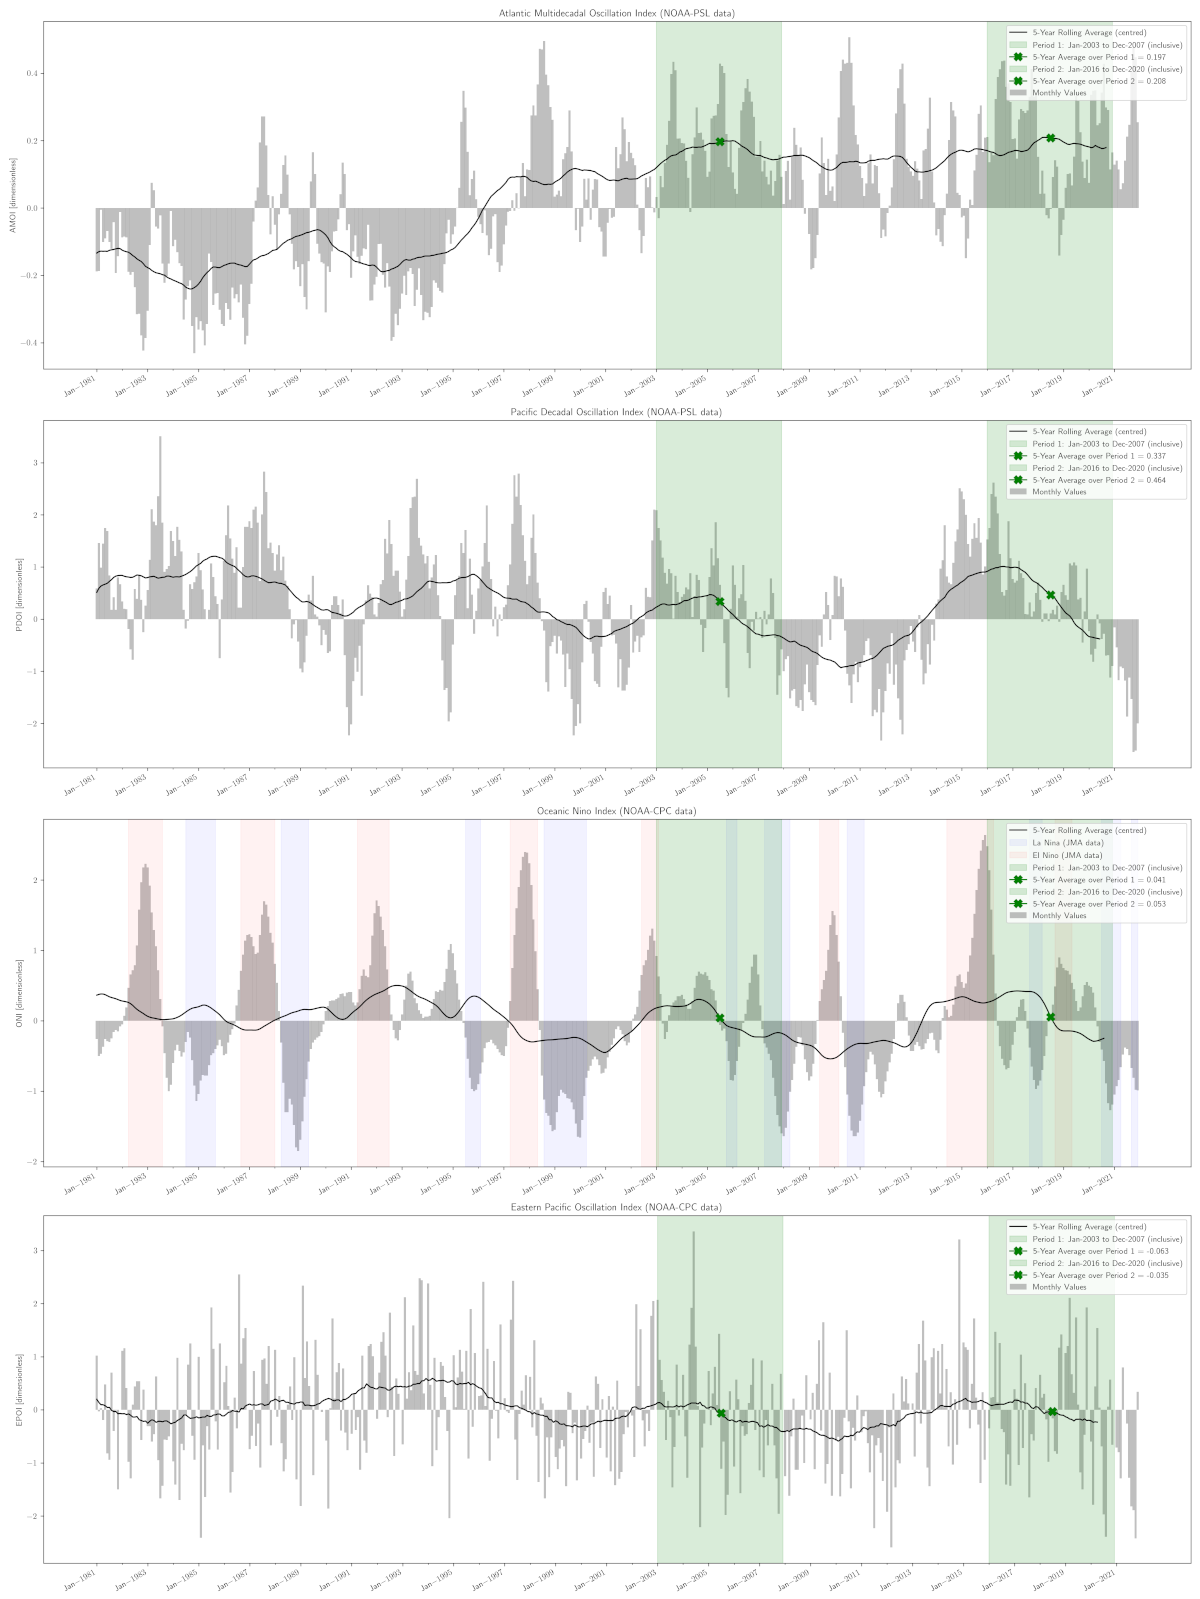
\includegraphics[width=0.9\textwidth]{ca_ind.png}
	\caption[CA's and SA's relevant climate indices for similar comparison]{\ac{NOAA} climate indices for climate drivers in \ac{CA}. Green shading highlights selected periods. Blue and red shading highlight La Nina and El Nino events respectively.}
	\label{fig:ca_ind}
\end{figure}

\paragraph{Very similar values and trends in climate indices}

The pair of Jan-2002 to Dec-2006 and Jan-2014 to Dec-2018 was deemed most appropriate since these periods had comparable averages in relevant climate indices and appear to span across the same phase of the relevant atmospheric oscillations. This was true for all of the relevant indices: \ac{AMOI}, \ac{PDOI}, \ac{ONI} (for \ac{ENSO}), and the \ac{EPOI}. The \ac{AOI} and \ac{NAOI} over these periods (not shown) also appeared to span across the same phase but had 5-year averages with slightly higher disparities (but these disparities were nevertheless small in terms of the characteristic size of the oscillations). The \ac{DMI} and the \ac{AAOI} (not shown) over these periods, on the other hand, were considerably different, but these were assumed not to be a major factor due to the distance of the Indian Ocean and Antarctica from the Americas\footnote{Significant effects due to teleconnections are theoretically possible but we have assumed this isn't the case here}.

\paragraph{Summary of El Nino-Southern Oscillation events}

The similarity between these periods is particularly remarkable because even the monthly values and 5-year averages for the \ac{ONI} (which has irregular oscillations) display a similar time evolution pattern. Both periods begin with the conclusion of an El Nino event and end past halfway into an La Nina event, and fully covers another La Nina event in between. The period from Jan-2014 to Dec-2018 contains an additional El Nino event not found in the period from Jan-2002 to Dec-2006 but this appears to mostly be a technicality with the definition of an El Nino event. A look at the monthly values reveals a spike in the \ac{ONI} which could have qualified as an El Nino event under slightly relaxed definitions. Furthermore, the monthly values between the starting El Nino event and ending La Nina event are almost mirror images of each other.

\paragraph{Time difference between periods well suited for studying land cover change}

In the case of Costa Rica, although remote sensing indicates that the rate of forest cover increase here was highest during the 1990s, leaf area index data derived from the \ac{AVHRR} instrument (not shown) for this region showed considerable noise and disagreement with \ac{MODIS} (the more advanced instrument). Given these factors, this set of study periods was also desirable because it was completely contained within the \ac{MODIS} coverage period. In addition to this, a land cover classification study by \citet{marx2017} using Landsat and \ac{UAV} data in lowland Costa Rica suggested an 11-year period for a pasture to transition into secondary forest, so a 13 year difference between selected periods corresponds well with our goals for studying the effects of \ac{LCC}. The change in \ac{MLAI} between these periods is displayed in Figure~\ref{fig:ca_lai_similar}.

\begin{figure}[!ht]
	\centering
	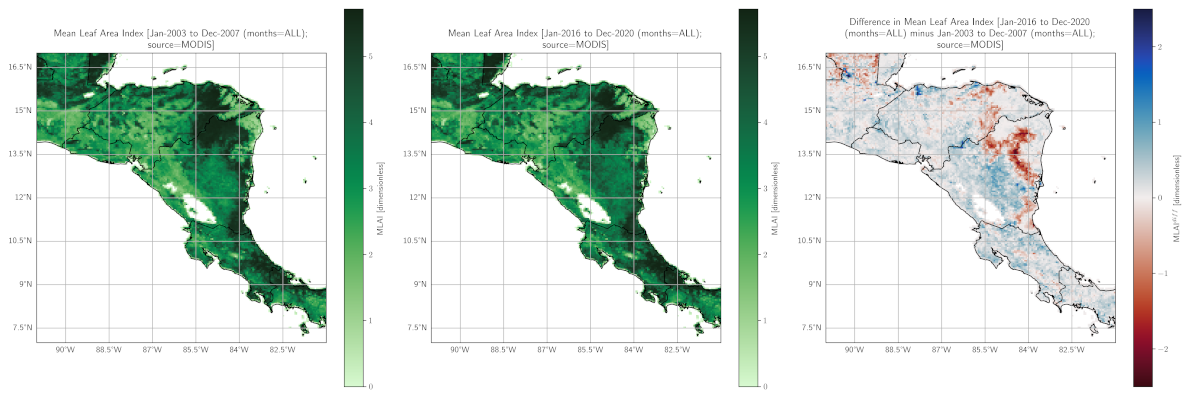
\includegraphics[width=0.9\textwidth]{ca_lai_similar.png}
	\caption[MLAI similar comparison for CA focus region]{\ac{MLAI} computed over each period in the similar comparison (left and middle), as well as the difference in these values between the two periods (right).}
	\label{fig:ca_lai_similar}
\end{figure}

\subsubsection{Land use and land cover change}

Figure~\ref{fig:lc_ca} displays trends in \ac{LULCC} at around the time of period 1 in the similar comparison.

\begin{figure}[!ht]
	\centering
	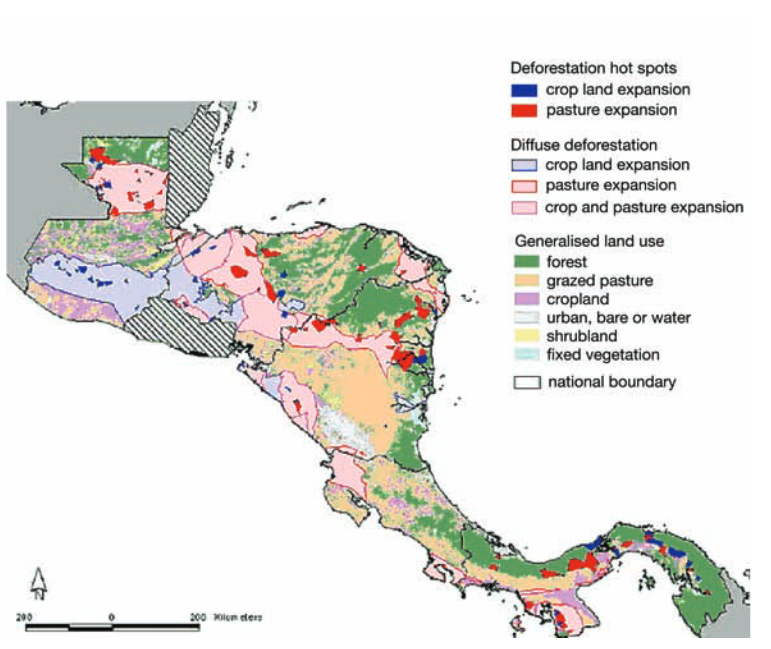
\includegraphics[width=0.75\textwidth]{lc_ca}
	\caption[Central America Land Usage]{Land usage and land cover change in Central America \citep{ipcc_2007}.}
	\label{fig:lc_ca}
\end{figure}

\subsection{Northern Brazil}

\begin{figure}[!ht]
	\centering
	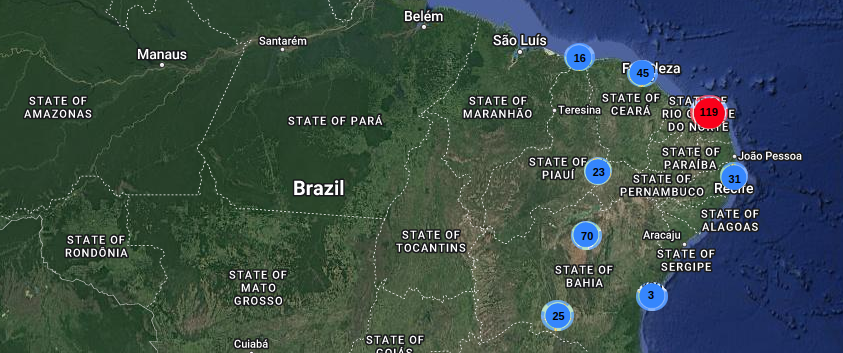
\includegraphics[width=0.75\textwidth]{maps_twp_sa}
	\caption[Northern Brazil Map]{Satellite image displaying Northern Brazil focus region from 65$^\circ$W to 30$^\circ$W longitude and 15$^\circ$S to 0$^\circ$S latitude \citep{maps_sa}. Markers indicating positions and number of wind farms have been edited on using data from \citep{twp_br}.}
	\label{fig:maps_twp_sa}
\end{figure}

\subsubsection{Description of region}

We selected the North to Northeast regions of Brazil (65$^\circ$W to 30$^\circ$W longitude and 15$^\circ$S to 0$^\circ$S latitude; see Figure~\ref{fig:maps_twp_sa}) because there has been extensive deforestation over this area and it was believed that effects resulting from \ac{LCC} here were likely to be especially pronounced. The change in \ac{MLAI} between these periods is displayed in Figure~\ref{fig:sa_lai_similar}.

\begin{figure}[!ht]
	\centering
	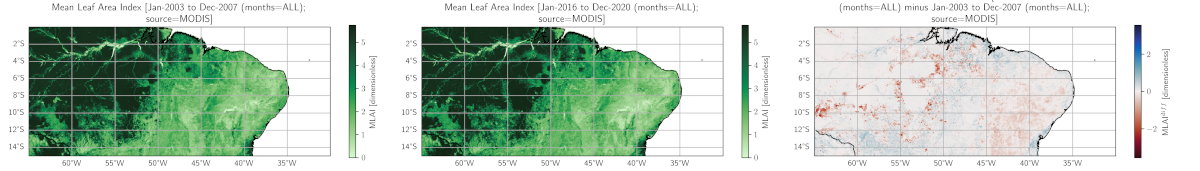
\includegraphics[width=0.9\textwidth]{sa_lai_similar.png}
	\caption[MLAI similar comparison for NB focus region]{\ac{MLAI} computed over each period in the similar comparison (left and middle), as well as the difference in these values between the two periods (right).}
	\label{fig:sa_lai_similar}
\end{figure}

\subsubsection{Significance of results from this region}

Several studies have identified large-scale changes in precipitation and moisture convergence patterns, which indirectly implicate surface wind changes. Effects here are likely to have immediate implications for energy generation due to the number of wind farms in this region (both existing and in the development pipeline\footnote{Up to 60 GW of offshore wind near the northeastern coast is in the early planning stage \citep{offshore_map}.}).

\subsubsection{Study periods}

For \ac{NB}, the selected periods for the similar comparison was from Jan-2002 to Dec-2006 and from Jan-2014 to Dec-2018 (for the same reasons highlighted in Section~\ref{sssec:period_seas_ca} for \ac{CA}.

\subsubsection{Land use and land cover change}

Figure~\ref{fig:lc_sa} displays trends in \ac{LULCC} at around the time of period 1 in the similar comparison.

\begin{figure}[!ht]
	\centering
	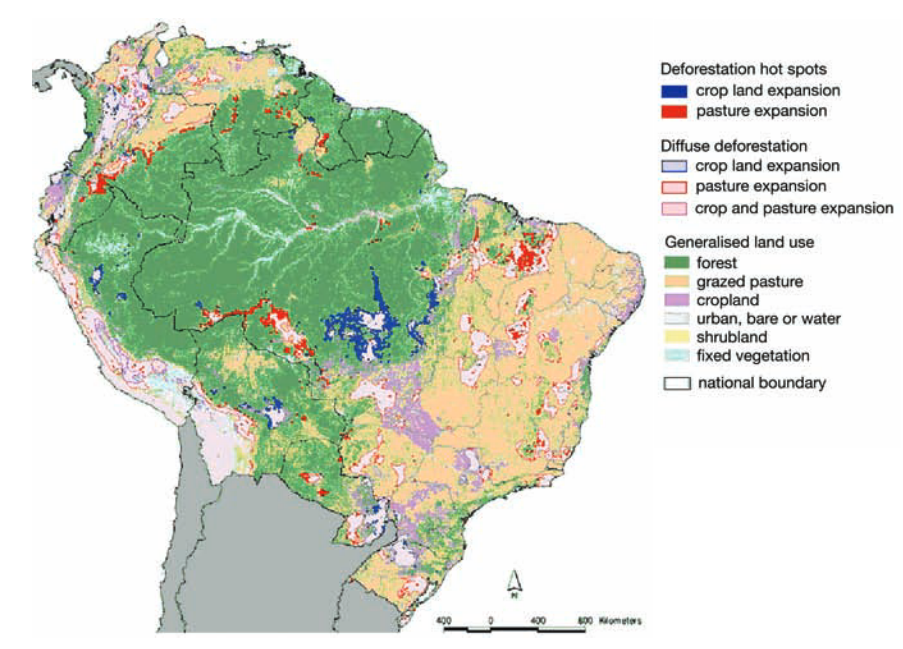
\includegraphics[width=0.75\textwidth]{lc_sa}
	\caption[Northern Brazil Land Usage]{Land usage and land cover change in Northern South America \citep{ipcc_2007}.}
	\label{fig:lc_sa}
\end{figure}     % these are just test names as I didn't know what you'd want
        \chapter{Data, files and codebooks}
\label{app:code}

\section{Availability and reproducible results}

\section{Description of analysis functions}

\blindtext[10]
    
        \chapter{Codebook and reproducibility}
\label{app:code}

All code created in the course of this project is available at \url{https://github.com/anthonylst6/thesis}. Programs created for automating analysis of an arbitrary \ac{ERA5} variable (in terms of mean diurnal profile statistics, hourly means and monthly means) were envisioned for general usage and as such, most of the functions within each script have been documented using Python docstrings, and permission to use these programs are granted subject to MIT License conditions.

\section{High-level description of functions}

\begin{itemize}
	\item The functions created in the course of this thesis allow comparison for the \acf{MLAI} and \acf{MFAPAR} between two arbitrary periods (so long as they are within the range of available data from 1981-2021). And the comparison can further be done in terms of a subset of months from each period. So it is possible, for example, to compare the \ac{MLAI} over the months of January, March and December between 1990-2000 with the \ac{MLAI} over the months of July and November between 2005-2007. These variables derive from the \ac{GLASS} dataset.
	\item These functions also allow comparison for various \ac{ERA5} variables between two arbitrary periods in terms of each variable's diurnal profile (can choose subset of months), mean (can choose subset of both months and hours), hourly means for each hour of the day (can choose subset of months), and monthly means for each month of the day (can choose subset of hours).
	\item For wind speed, there is also a separate function to compute the mean, standard deviation, Weibull distribution parameters resulting from an empirical fit, and other.
	\item The main data processing functions are contained in the \verb+calc_funcs.py+ script in the \verb+scripts+ folder.
	\item The \verb+plot_funcs.py+ script in the \verb+scripts+ folder is a plotting layer on top of \verb+calc_funcs.py+ and contains all the functions for creating comparison plots.
	\item Most analysis can be done purely using the \verb+plot_funcs.py+ script since this was built to automatically invoke any processing functions from \verb+calc_funcs.py+ if the processed data file does not already exist.
	\item The entire code is built around carefully selected names for each file, so it is not recommended to rename any of these files as this may break the code.
	\item There is a vast array of functions within these scripts but we will describe here only the high-level comparison plot functions. For detail into the other functions, look into the docstrings embedded within each script. At the time of writing, \verb+calc_funcs.py+ is fully documented while only the high-level comparison plot functions in \verb+plot_funcs.py+ have been documented.
	\item The high-level comparison plot functions in \verb+plot_funcs.py+ are: 
	\begin{itemize}
		\item \verb+plot_comp_mdp_clim_stats_given_var_or_dvar+
		\item \verb+plot_comp_means_given_layer_and_type+
		\item \verb+plot_comp_hourly_means_given_var_or_dvar+
		\item \verb+plot_comp_monthly_means_given_var_or_dvar+
		\item \verb+plot_comp_wsd_clim+
	\end{itemize}
	\item Each of these functions creates an output plot with 3 columns and 8 rows. The left column corresponds to the statistical summaries for the first period of study. The middle column is the same but for the second period. The right column is the difference between periods in the values for each statistical summary (calculated as second period minus first period). For reference, the first two rows will always display \ac{MLAI} and \ac{MFAPAR}. The colourbars are automatically standardised to allow fair comparison between periods, months and hours.
	\item Where spatiotemporal correlations in the left or middle columns hold between an \ac{ERA5} statistic and \ac{MLAI}, this is suggestive that the vegetation cover \textit{may} be responsible for the observed variations in the \ac{ERA5} statistic.
	\item Where spatiotemporal correlations hold between the right column of an \ac{ERA5} statistic and the left or middle columns for \ac{MLAI}, this leaves open the question of what is causing the observed variations in the \ac{ERA5} statistic, but suggests that vegetation cover \textit{may} be responsible for modulating these variations.
	\item Where spatiotemporal correlations hold between the right columns of an \ac{ERA5} statistic and \ac{MLAI}, this is suggestive that the variations in vegetation cover \textit{may} be responsible for the variations in the \ac{ERA5} statistic.
\end{itemize}

\section{Example usage}

\subsection{plot\_comp\_mdp\_clim\_stats\_given\_var\_or\_dvar}

Suppose we were interested in analysing the seasonal differences in the diurnal statistics of mean sea level pressure ("mslp") in a region of South America ("sa"), with default region extents manually defined in the \verb+calc_funcs.py+ script. Specifically, we are interested in differences between the wet season from January to June ([1,2,3,4,5,6]) and the dry season from July to December ([7,8,9,10,11,12]), over the period from "Jan-2001" to "Dec-2020". Then we would use the following code to obtain Figure~\ref{fig:plot_comp_mdp_clim_stats_given_var_or_dvar}:

\begin{lstlisting}[language=Python,caption={Example for plot\_comp\_mdp\_clim\_stats\_given\_var\_or\_dvar},captionpos=b]
	import plot_funcs_v1h as pf
	pf.plot_comp_mdp_clim_stats_given_var_or_dvar(
		region="sa", period1_start="Jan-2001", period1_end="Dec-2020", 
		period2_start="Jan-2001", period2_end="Dec-2020", 
		period1_months=[1,2,3,4,5,6], period2_months=[7,8,9,10,11,12], 
		glass_source_pref="modis", var_or_dvar="mslp", 
		perc=False, mask_perc_quantile=pf.mask_perc_quantile_default, 
		mask_period1=None, mask_period2=None, extents=None, cfv_data=None, 
		output=True
	)
\end{lstlisting}

\begin{figure}[!htp]
	\centering
	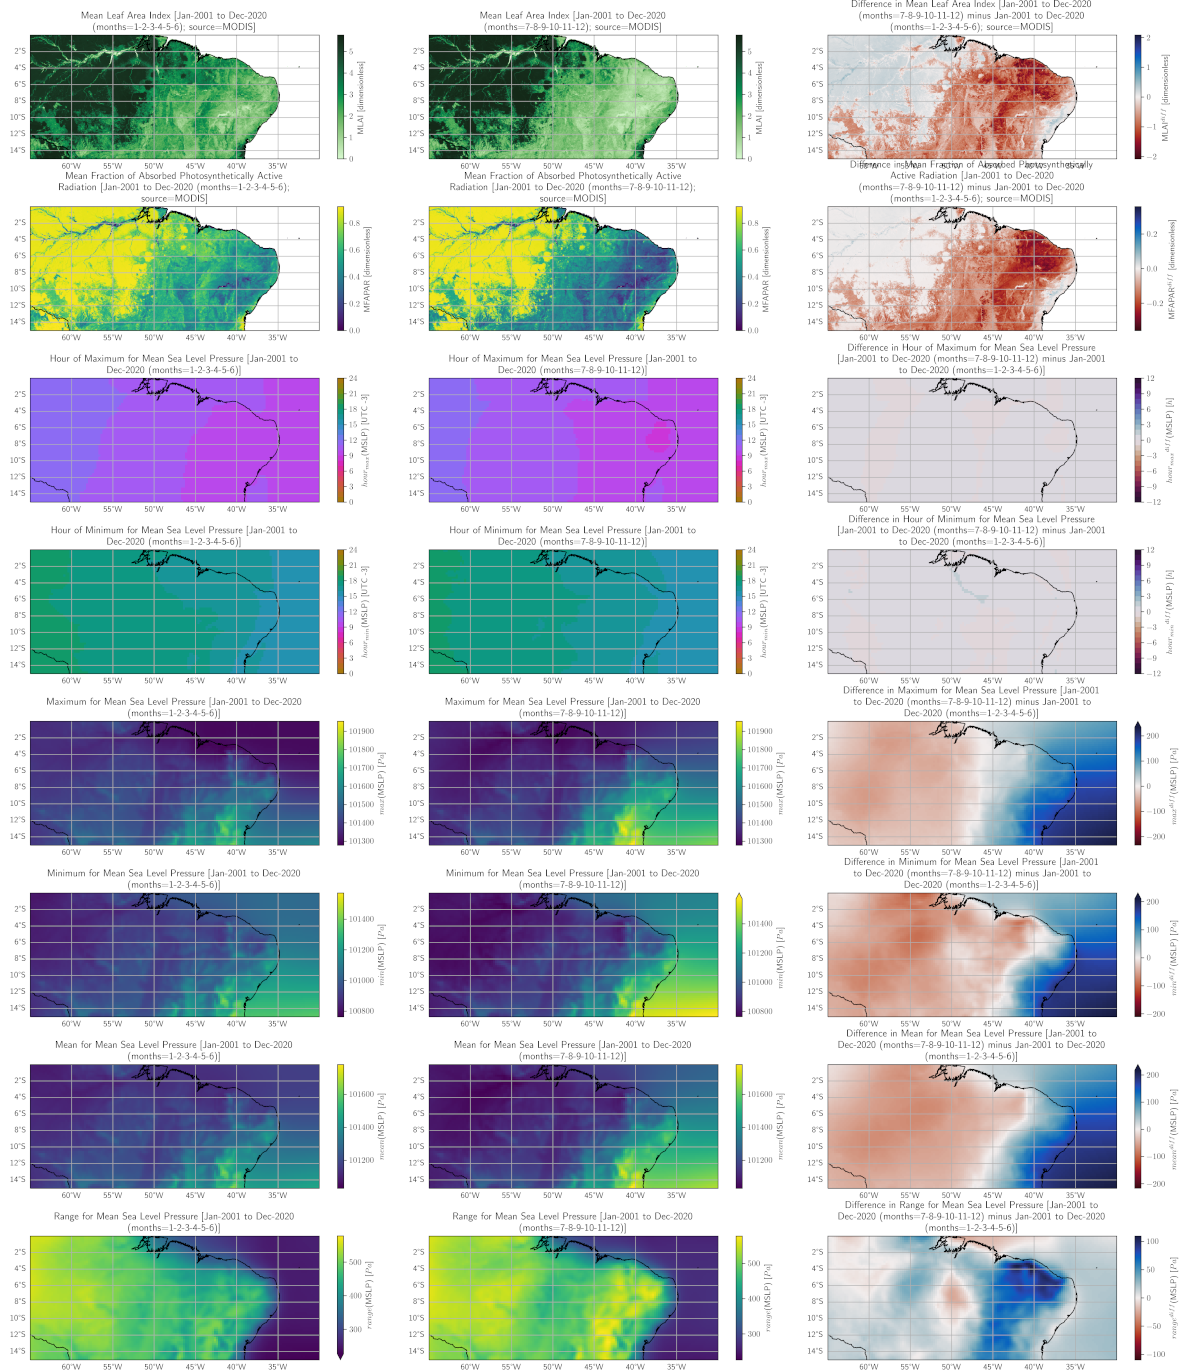
\includegraphics[width=0.9\textwidth]{plot_comp_mdp_clim_stats_given_var_or_dvar}
	\caption{Example for plot\_comp\_hourly\_means\_given\_var\_or\_dvar}
	\label{fig:plot_comp_mdp_clim_stats_given_var_or_dvar}
\end{figure}

\subsection{plot\_comp\_means\_given\_layer\_and\_type}

Suppose we were interested in analysing differences in the means between two separate periods for the hourly change in variables ("dvars") at the surface ("sfc"), in a region of Central America ("ca"), with default region extents manually defined in the \verb+calc_funcs.py+ script. Specifically, we are interested in differences in means computed over daytime hours from 0800 to 1500 ([8,9,10,11,12,13,14,15]) and the wet season from May to October ([5,6,7,8,9,10]), between the periods from "Jan-2003" to "Dec-2007" and "Jan-2016" to "Dec-2020". Then we would use the following code to obtain Figure~\ref{fig:plot_comp_means_given_layer_and_type}:

\begin{lstlisting}[language=Python,caption={Example for plot\_comp\_means\_given\_layer\_and\_type},captionpos=b]
	import plot_funcs_v1h as pf
	pf.plot_comp_means_given_layer_and_type(
		region="ca", period1_start="Jan-2003", period1_end="Dec-2007", 
		period2_start="Jan-2016", period2_end="Dec-2020", 
		period1_months=[5,6,7,8,9,10], period2_months=[5,6,7,8,9,10], 
		period1_hours=[8,9,10,11,12,13,14,15], 
		period2_hours=[8,9,10,11,12,13,14,15], 
		glass_source_pref="modis", 
		var_or_dvar_layer="sfc", var_or_dvar_type="dvars", 
		perc=False, mask_perc_quantile=pf.mask_perc_quantile_default, 
		mask_period1=None, mask_period2=None, extents=None, cfv_data=None, 
		output=True
	)
\end{lstlisting}

\begin{figure}[!htp]
	\centering
    \begin{subfigure}[!htp]{0.9\textwidth}
		\centering
		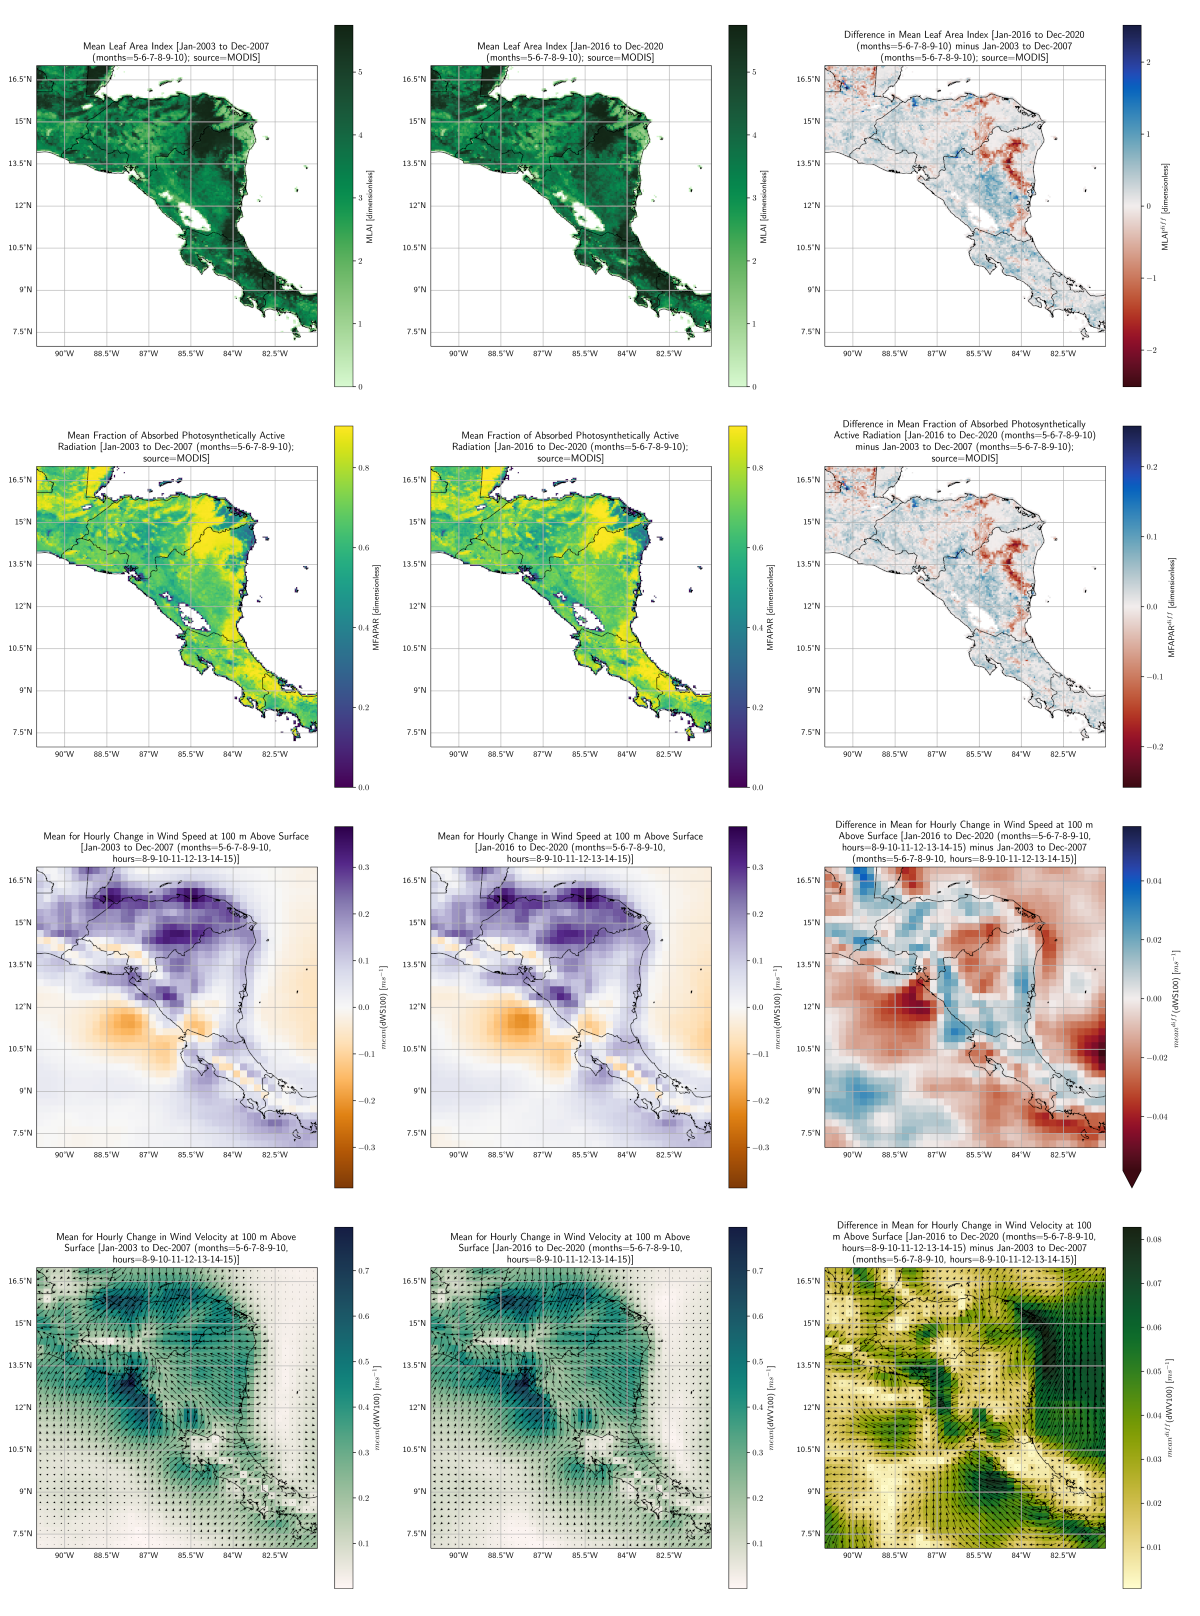
\includegraphics[width=0.9\textwidth]{plot_comp_means_given_layer_and_type_1}
		\caption[]{First 4 rows of example plot}
	\end{subfigure}
\end{figure}

\begin{figure}[!htp]\ContinuedFloat
    \begin{subfigure}[!htp]{0.9\textwidth}
		\centering
		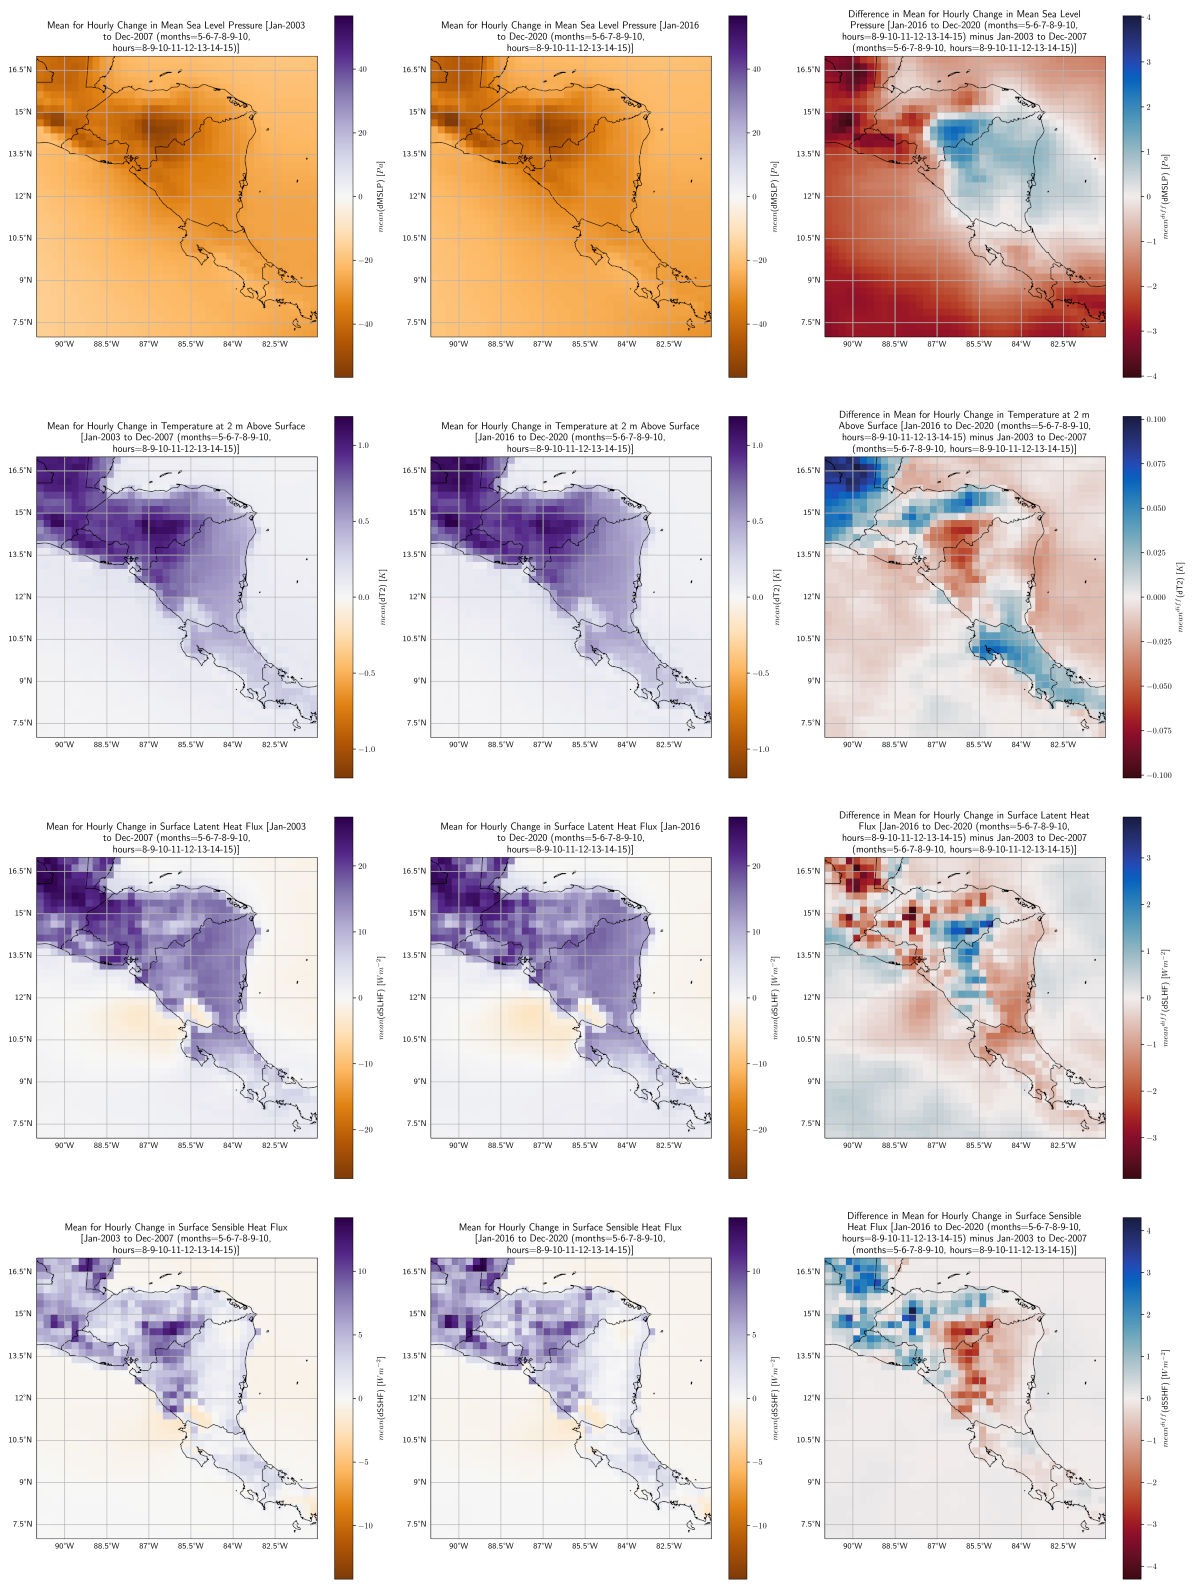
\includegraphics[width=0.9\textwidth]{plot_comp_means_given_layer_and_type_2}
		\caption[]{Last 4 rows of example plot}
	\end{subfigure}
	\caption{Example for plot\_comp\_means\_given\_layer\_and\_type}
	\label{fig:plot_comp_means_given_layer_and_type}
\end{figure}

\subsection{plot\_comp\_hourly\_means\_given\_var\_or\_dvar}

Suppose we were interested in analysing the seasonal differences in the hourly means of vertical integral of energy conversion ("viec") in a region of Western Australia ("wa"), with default region extents manually defined in the \verb+calc_funcs.py+ script (and the State Boundary Fence of Western Australia is drawn in). Specifically, we are interested in differences between the wet season from July to August ("jja") and the dry season from December to February ("djf"), over the period from "Jan-2001" to "Dec-2020". Then we would use the following code to obtain Figure~\ref{fig:plot_comp_hourly_means_given_var_or_dvar}:

\begin{lstlisting}[language=Python,caption={Example for plot\_comp\_hourly\_means\_given\_var\_or\_dvar},captionpos=b]
	import plot_funcs_v1h as pf
	pf.plot_comp_hourly_means_given_var_or_dvar(
		region="wa", period1_start="Jan-2001", period1_end="Dec-2020", 
		period2_start="Jan-2001", period2_end="Dec-2020", 
		period1_months="jja", period2_months="djf", glass_source_pref="modis", 
		var_or_dvar="viec", hours_to_plot="18-23", 
		perc=False, mask_perc_quantile=pf.mask_perc_quantile_default, 
		mask_period1=None, mask_period2=None, extents=None, cfv_data=None, 
		output=True
	)
\end{lstlisting}

\begin{figure}[!htp]
	\centering
	\begin{subfigure}[!htp]{0.9\textwidth}
		\centering
		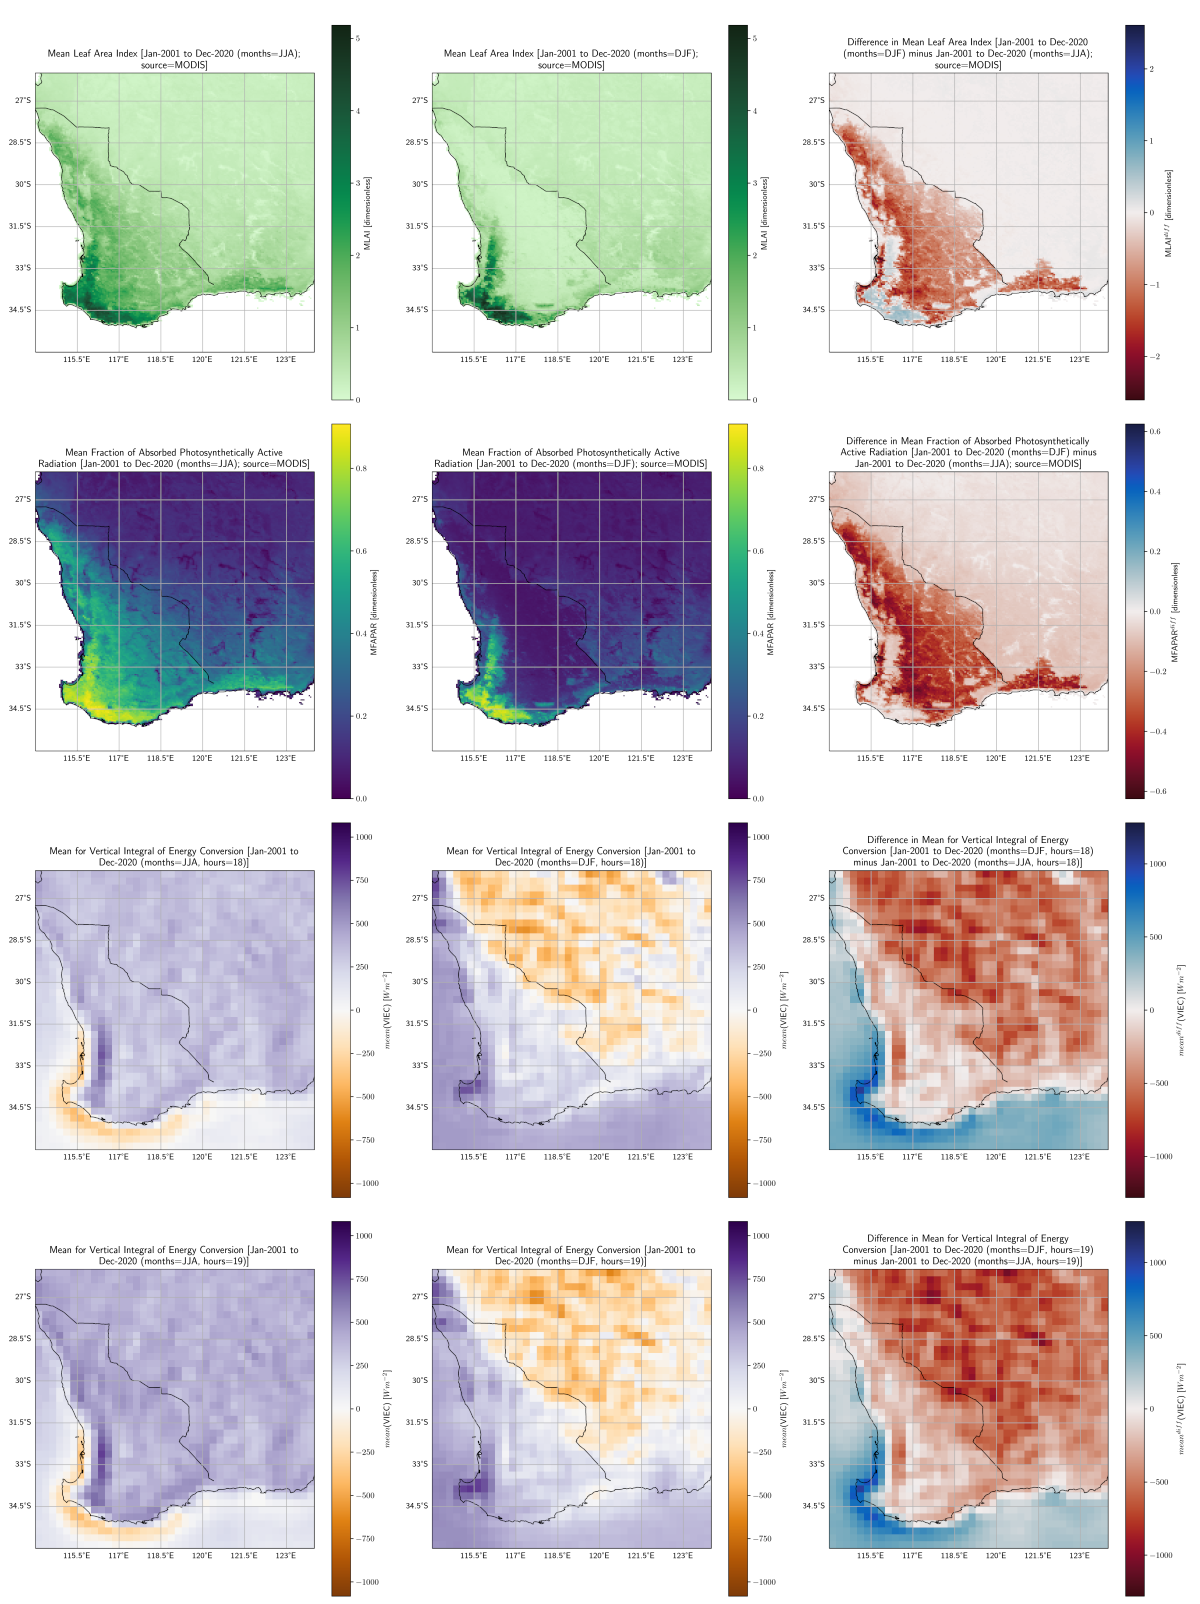
\includegraphics[width=0.9\textwidth]{plot_comp_hourly_means_given_var_or_dvar_1}
		\caption[]{First 4 rows of example plot}
	\end{subfigure}
\end{figure}

\begin{figure}[!htp]\ContinuedFloat
	\begin{subfigure}[!htp]{0.9\textwidth}
		\centering
		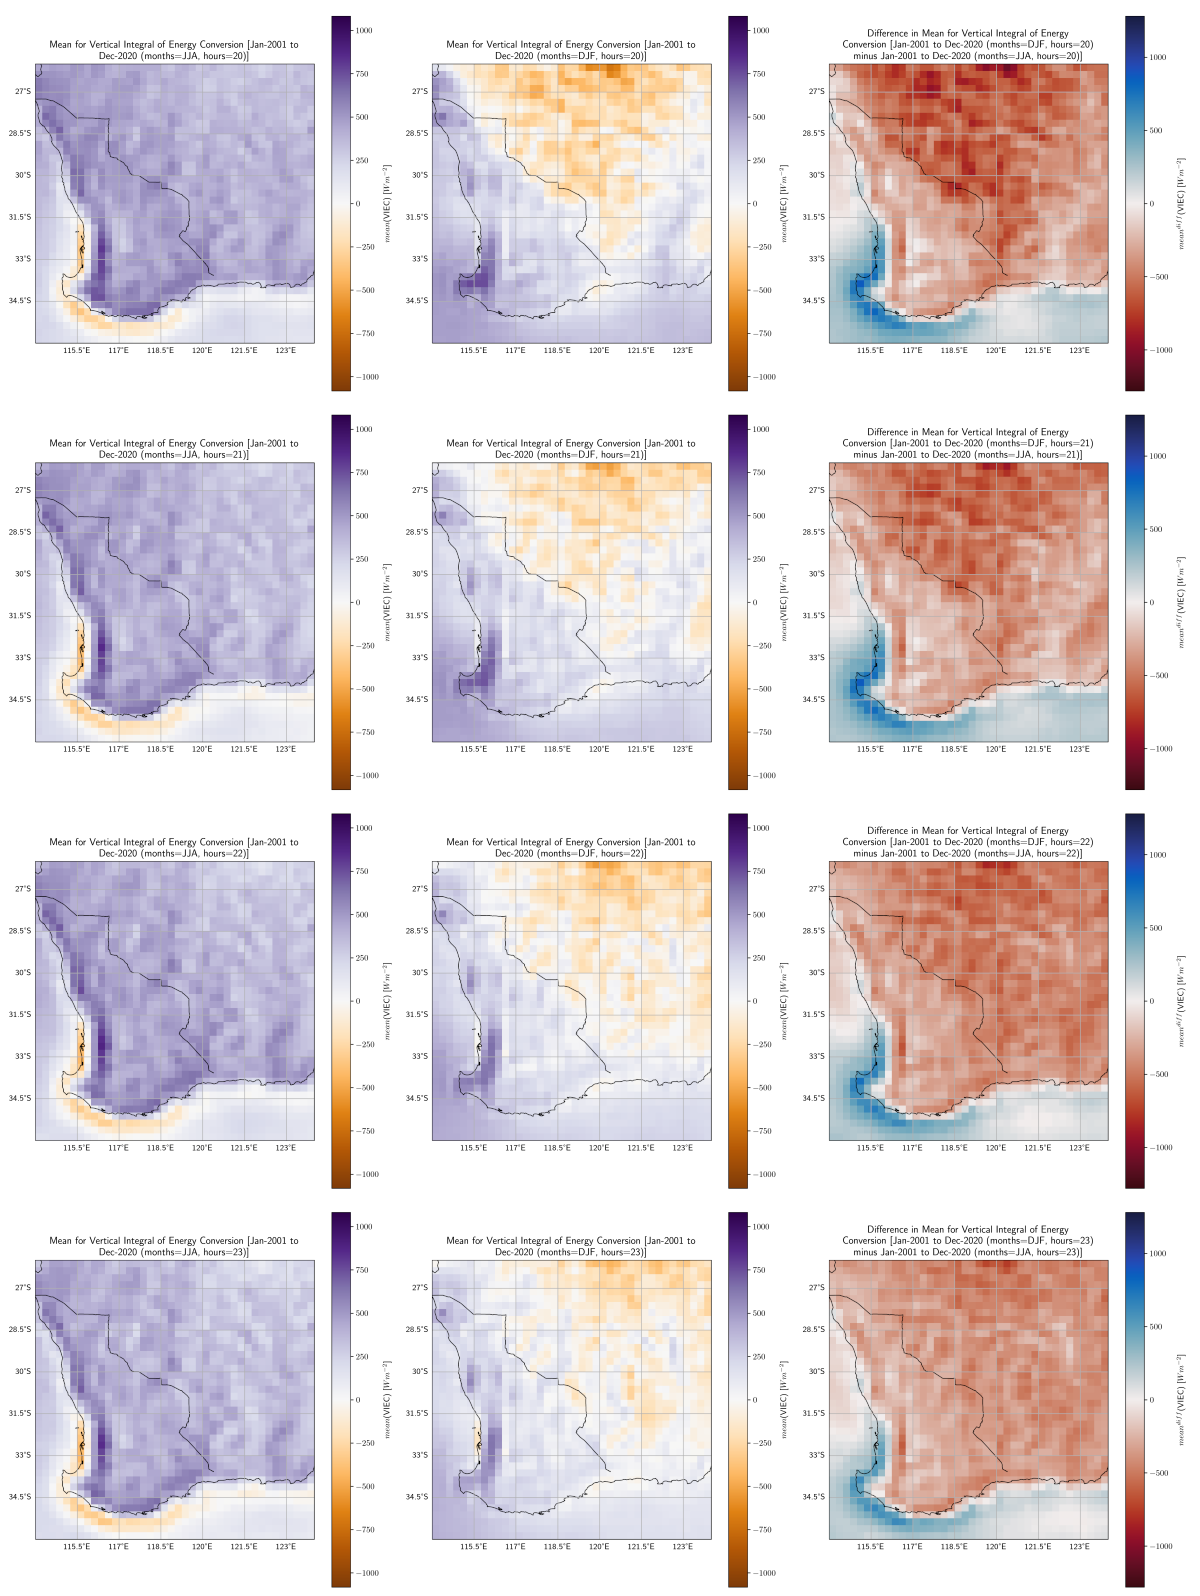
\includegraphics[width=0.9\textwidth]{plot_comp_hourly_means_given_var_or_dvar_2}
		\caption[]{Last 4 rows of example plot}
	\end{subfigure}
	\caption{Example for plot\_comp\_hourly\_means\_given\_var\_or\_dvar}
	\label{fig:plot_comp_hourly_means_given_var_or_dvar}
\end{figure}

\section{Analysing other regions and variables}

Note: the steps in this section have not been tested as of the time of writing.

\subsection{For custom regions}

\begin{itemize}
	\item The default regions and extents in [W, E, S, N] format (for \verb+cartopy+ plotting library) used in the thesis project were: 
	\begin{itemize}
		\item "wa": [114, 124, -36, -26]
		\item "ca": [-91, -81, 7, 17]
		\item "sa": [-65, -30, -15, 0]
	\end{itemize}
	\item To add a custom region:
	\begin{enumerate}
		\item Edit the \verb+area+ variable in \verb+data_download.ipynb+ or \verb+data_download.py+ to include the name of the new region and its extents in [N, W, S, E] format (for \ac{ECMWF} \ac{CDS} API)
		\item Edit the first argument in the \verb+retrieve_era5_slv_month_hour+ and \\ \verb+retrieve_era5_slv_hour+ functions so that it reflects the name of the new region
		\item Run the edited \verb+data_download.ipynb+ or \verb+data_download.py+ to download the relevant \ac{ERA5} data from \ac{ECMWF}
		\item Edit the \verb+regions+ variable in the \verb+calc_funcs.py+ script to include the new region's name, extents in [W, E, S, N] format, and local timezone relative to UTC
	\end{enumerate}
\end{itemize}

\subsection{For arbitrary ERA5 variables}

\begin{itemize}
	\item The ERA5 variables obtained from \ac{ECMWF} for use in the thesis project by default were (using naming conventions from \url{https://confluence.ecmwf.int/display/CKB/ERA5%3A+data+documentation}):
		\begin{itemize}
			\item \verb+'100m_u_component_of_wind'+
			\item \verb+'100m_v_component_of_wind'+
			\item \verb+'10m_u_component_of_wind'+
			\item \verb+'10m_v_component_of_wind'+
			\item \verb+'2m_temperature'+
			\item \verb+'mean_sea_level_pressure'+
			\item \verb+'surface_latent_heat_flux'+
			\item \verb+'surface_sensible_heat_flux'+
			\item \verb+'evaporation'+
			\item \verb+'total_column_cloud_liquid_water'+
			\item \verb+'total_column_water_vapour'+
			\item \verb+'vertical_integral_of_divergence_of_moisture_flux'+
			\item \verb+'vertical_integral_of_energy_conversion'+
			\item \verb+'vertical_integral_of_kinetic_energy'+
			\item \verb+'convective_inhibition'+
			\item \verb+'forecast_albedo'+
			\item \verb+'total_cloud_cover'+
		\end{itemize}
	\item To add an arbitrary \ac{ERA5} variable:
	\begin{enumerate}
		\item Edit the \verb+vars_era5+ variable in \verb+data_download.ipynb+ or \\ \verb+data_download.py+ to include the name of the new variable using the \ac{ERA5} variable names from \url{https://confluence.ecmwf.int/display/CKB/ERA5%3A+data+documentation}
		\item Place the variable within one of the existing "sfc", "atm" or "cld" categories
		\item (Alternatively) Create a new category with the variable and add additional code cells with the new category name as an argument into the \\ \verb+retrieve_era5_slv_month_hour+ and \\ \verb+retrieve_era5_slv_hour functions+
		\item Run the edited \verb+data_download.ipynb+ or \verb+data_download.py+ to download the relevant \ac{ERA5} data from \ac{ECMWF} \ac{CDS}
		\item Edit the \verb+vars_and_dvars_era5+, \verb+vars_dep_and_rename+ and \verb+attrs_da+ variables in the \verb+calc_funcs.py+ script to reflect this new variable
		\item Edit the try-except blocks in the \verb+plot_means_given_layer_and_type+, \verb+plot_diff_means_given_layer_and_type+ and \\ \verb+plot_comp_means_given_layer_and_type+ functions in the \\ \verb+plot_funcs.py+ script so that a total of 6 \ac{ERA5} variables will be displayed at all times (this is an unfortunate design constraint from displaying 8 rows for the comparison plots with the first 2 rows occupied by \ac{MLAI} and \ac{MFAPAR})
	\end{enumerate}
\end{itemize}

\subsection{For novel ERA5-derived variables}

\begin{itemize}
	\item The default \ac{ERA5}-derived variables used in the thesis project were: 
	\begin{itemize}
		\item Instantaneous approximation (with negative sign reversed and units converted) for \acf{SLHF}
		\item Instantaneous approximation (with negative sign reversed and units converted) for \acf{SSHF}
		\item Instantaneous approximation (with negative sign reversed and units converted) for \acf{NSE}
		\item Approximation for \acf{NAC}
	\end{itemize}
	\item To incorporate a novel \ac{ERA5}-derived variable:
	\begin{enumerate}
		\item Insert an if statement into the \verb+calc_era5_mdp_clim_given_var_or_dvar+ function in the \verb+calc_funcs.py+ script (this is the function which is furthest upstream and from which other computations apart from wind speed distribution derive from) using the same style and logic as that for \ac{NAC} in the script
		\item Edit the \verb+vars_and_dvars_era5+, \verb+vars_dep_and_rename+ and \verb+attrs_da+ variables in the \verb+calc_funcs.py+ script to reflect this new variable
		\item Edit the try-except blocks in the \verb+plot_means_given_layer_and_type+, \verb+plot_diff_means_given_layer_and_type+ and \\ \verb+plot_comp_means_given_layer_and_type+ functions in the \\ \verb+plot_funcs.py+ script so that a total of 6 ERA5 variables will be displayed at all times (this is an unfortunate design constraint from displaying 8 rows for the comparison plots with the first 2 rows occupied by \ac{MLAI} and \ac{MFAPAR})
	\end{enumerate}
\end{itemize}

\section[Steps to reproduce thesis]{Steps to reproduce thesis results from scratch}

Note: The original project scope included analysis for \ac{WA}, \ac{CA} and \ac{NB} but this was cut short to only \ac{WA} due to time constraints.

\begin{enumerate}
	\item (If haven't already) Install miniconda for Python 3.9 or later using instructions from \url{https://docs.conda.io/en/latest/miniconda.html}
	\item Download thesis repository by entering \\ \verb+git clone git@github.com:anthonylst6/thesis.git+ into a bash shell (Terminal for Linux or Mac, Git Bash recommended for Windows) or clicking Code -> Download ZIP on Github then unzip the folder
	\item Open bash shell in home directory of repository then run \\ \verb+conda env create -f env_thesis.yml+
	\item (If haven't already) Set up \ac{ECMWF} \ac{CDS} API using instructions from \url{https://confluence.ecmwf.int/display/CKB/How+to+download+ERA5#HowtodownloadERA5-4-DownloadERA5familydatathroughtheCDSAPI}
	\item Download raw data by entering \verb+conda activate thesis+ into bash shell then running the \verb+data_download.ipynb+ notebook in the \verb+scripts+ directory (open the notebook by running \verb+jupyter lab &+ in the bash shell)
	\item (Alternatively) Enter \verb+conda run -n thesis python data_download.py+ \\ into bash shell from the \verb+scripts+ directory
	\item (For proper rendering of figures) Make sure that a \LaTeX distribution is installed
	\item Reproduce results by running the \verb+results.ipynb+ notebook in the \verb+scripts+ directory for different focus regions by commenting and uncommenting relevant code (again use \verb+jupyter lab &+ from bash shell to open notebooks)
	\item (Alternatively) Enter \verb+conda run -n thesis python results_wa.py+, \\ \verb+conda run -n thesis python results_ca.py+ and \\ \verb+conda run -n thesis python results_sa.py+ into bash shell from the \\ \verb+scripts+ directory
	\item (If personal computer is limited in RAM) Edit the \verb+results_wa.pbs+, \\ \verb+results_ca.pbs+ and \verb+results_sa.pbs+ job scripts in the \verb+scripts+ directory to be compatible with target HPC facility (the provided scripts were designed for the UNSW Katana computational cluster), then submit these as a batch job
\end{enumerate}

\section[System and time requirements]{System and time requirements (for reproducing thesis results only)}
\begin{itemize}
	\item For \acf{WA} raw data and results, up to 25 GB of storage, several days for raw data download (due to queueing in \ac{ECMWF} \ac{CDS}), and for data processing up to 60 GB of RAM over 12 hours if using 8 CPUs
	\item For \acf{CA} raw data and results, up to 25 GB of storage, several days for raw data download (due to queueing in \ac{ECMWF} \ac{CDS}), and for data processing up to 60 GB of RAM over 12 hours if using 8 CPUs
	\item For \acf{NB} raw data and results, up to 80 GB of storage, several days for raw data download (due to queueing in \ac{ECMWF} \ac{CDS}), and for data processing up to 140 GB of RAM over 12 hours if using 8 CPUs
	\item The data processing can also be run with less RAM and fewer CPU cores but this will be slower and will require manual restarting of code everytime RAM limit is reached (the code was designed to pick up from where it left off). But in this case there should at least be 8 GB of RAM for \ac{WA} and \ac{CA} results, and at least 24 GB of RAM for \ac{NB} results.
\end{itemize}
 

\pagestyle{umpageback}
{\backmatter
    % Bibliography
    \if@openright\cleardoublepage\else\clearpage\fi

    \bibliographystyle{um-plainnat} %% specific plainnat does not show url for articles
    % Use something like https://flamingtempura.github.io/bibtex-tidy/ to clean all your bibtex entries
    { 	\scriptsize\bibliography{chap1/introduction_biblio,chap2/literature_review_biblio,chap3/methodology_biblio,chap4/results_biblio,chap5/discussion_biblio,chap6/conclusions_biblio,appA/appendix_a_biblio,appB/appendix_b_biblio,appC/appendix_c_biblio}}
	\printindex
}

\end{document}

%%% The End %%%
